% !TeX spellcheck = pt_BR

\chapter{Gravitação}

Existe uma ironia histórica no fato de o capítulo de gravitação
aparecer aqui, nesta parte chamada de ``aplicações''. Porque, a bem
da verdade, a situação é o inverso: não foi que Newton inventou a
mecânica e depois a aplicou aos planetas. Foi que o problema dos
planetas \emph{forçou} Newton a inventar a mecânica. A gravitação
não é uma aplicação da Física Clássica --- ela é a sua razão de ser.
 
A história começa, como tantas na ciência, com dados e sem teoria.
Johannes Kepler, no início do século~XVII, passou anos debruçado
sobre as observações meticulosas de Tycho Brahe --- o maior
astrônomo do mundo pré-telescópio --- e delas extraiu três leis
que descrevem com precisão extraordinária o movimento dos planetas
ao redor do Sol. As leis de Kepler são um triunfo da indução:
padrões matematicamente precisos extraídos de medições, sem que
Kepler soubesse, de fato, \emph{por que} os planetas obedeciam
a esses padrões. Ele tinha a descrição; faltava a explicação. Veremos um pouco mais dessa história já no estudo da Equação \eqref{eq_gravitacao_terceiraleikepler}.
 
Newton chegou meio século depois com a explicação. Mas Newton fez
mais do que apenas explicar as leis de Kepler: ele mostrou que a
mesma força responsável por fazer a maçã cair de uma árvore era a
responsável por manter a Lua em órbita. Essa foi, talvez, a maior
unificação conceitual da história da ciência antes de Maxwell e
Einstein: o mesmo fenômeno, obedecendo à mesma equação matemática,
governava tanto a matéria mais próxima quanto os corpos mais
distantes do universo. O céu e a Terra, que desde Aristóteles eram
regidos por leis diferentes, passaram a ser vistos como partes de
um mesmo sistema físico.
 
Neste capítulo, faremos o percurso dessa história. Começaremos
pela Terceira Lei de Kepler --- uma lei experimental, fruto de
observação ---,  que será o nosso ponto de partida empírico. Em
seguida, veremos a Lei da Gravitação Universal de Newton, que
explica de onde Kepler veio e unifica os dois mundos. A partir
daí, as equações que seguem --- velocidade orbital, campo
gravitacional, energia potencial gravitacional, velocidade de
escape e energia total de uma órbita --- são todas derivadas dessa
lei fundamental, e constituem um dos edifícios teóricos mais
coerentes e belos que a Física já construiu.
 
O leitor vai notar que, ao longo deste capítulo, precisaremos das
\emph{duas linguagens da dinâmica}. Para calcular a velocidade com
que um satélite orbita a Terra, usaremos a linguagem vetorial: a
força gravitacional fornece a força centrípeta necessária para o
movimento circular. Para calcular a velocidade mínima com que um
foguete deve ser lançado a fim de escapar para sempre do campo
gravitacional terrestre, usaremos a linguagem escalar: a condição
é que a energia total do sistema seja nula. Essa alternância não
é coincidência --- é a gravitação nos mostrando que nenhuma das
duas linguagens é suficiente, por si só, para contar toda a história.
 
Vale deixar uma advertência final antes de começarmos. Newton
passou anos derivando e verificando a Lei da Gravitação Universal.
Quando os \emph{Principia} foram publicados, em 1687, ele a havia
demonstrado rigorosamente a partir das leis do movimento. E mesmo
assim, ao ser perguntado sobre o que \emph{era}, de fato, a
gravidade --- o que a causava, qual era o mecanismo físico por
trás da atração entre massas ---, Newton respondeu com uma das
frases mais honestas da história da ciência: \textit{hypotheses
non fingo} --- não forjo hipóteses.\footnote{Newton, I.
\textit{Philosophiæ Naturalis Principia Mathematica}, Escólio
Geral, 3ª~edição, 1726.} Ele sabia \emph{como} a gravidade agia.
Não sabia \emph{por quê}. E essa pergunta, de certa forma, só
seria respondida duzentos anos depois, por Einstein. Mas essa é
uma outra história --- e pertence a um outro livro.
 





















\section{Leis de Kepler e Gravitação}





\begin{secnivel}[Terceira Lei de Kepler]{I}{Terceira Lei de Kepler}
  
  \eqLdois{exp}{eq_gravitacao_terceiraleikepler}{ \dfrac{T^2}{R^3} = \text{ constante}}

\end{secnivel}


\secgfe{De onde vem}

A Terceira Lei de Kepler diz respeito a corpos que estejam orbitando em torno de um mesmo astro. Ela expressa uma condição que deve ser satisfeita pelo período de translação $T$ desses corpos (tempo para que eles completem uma volta em torno do astro central) e o raio médio de suas órbitas $R.$ A lei diz que, para todos esses corpos -- desde que estejam orbitando em torno do mesmo astro -- o quadrado do seu período dividido pelo cubo do seu raio médio dará sempre o mesmo valor.

No caso de órbitas circulares, o raio médio em questão será o próprio raio $R$ da circunferência. Para órbitas elípticas, o raio médio será igual ao semieixo maior $a$ da elipse, como mostra a Figura \ref{fig_gravitacao_3ndkeplerslaw}.



\vspace{0.3cm}
{
\centering
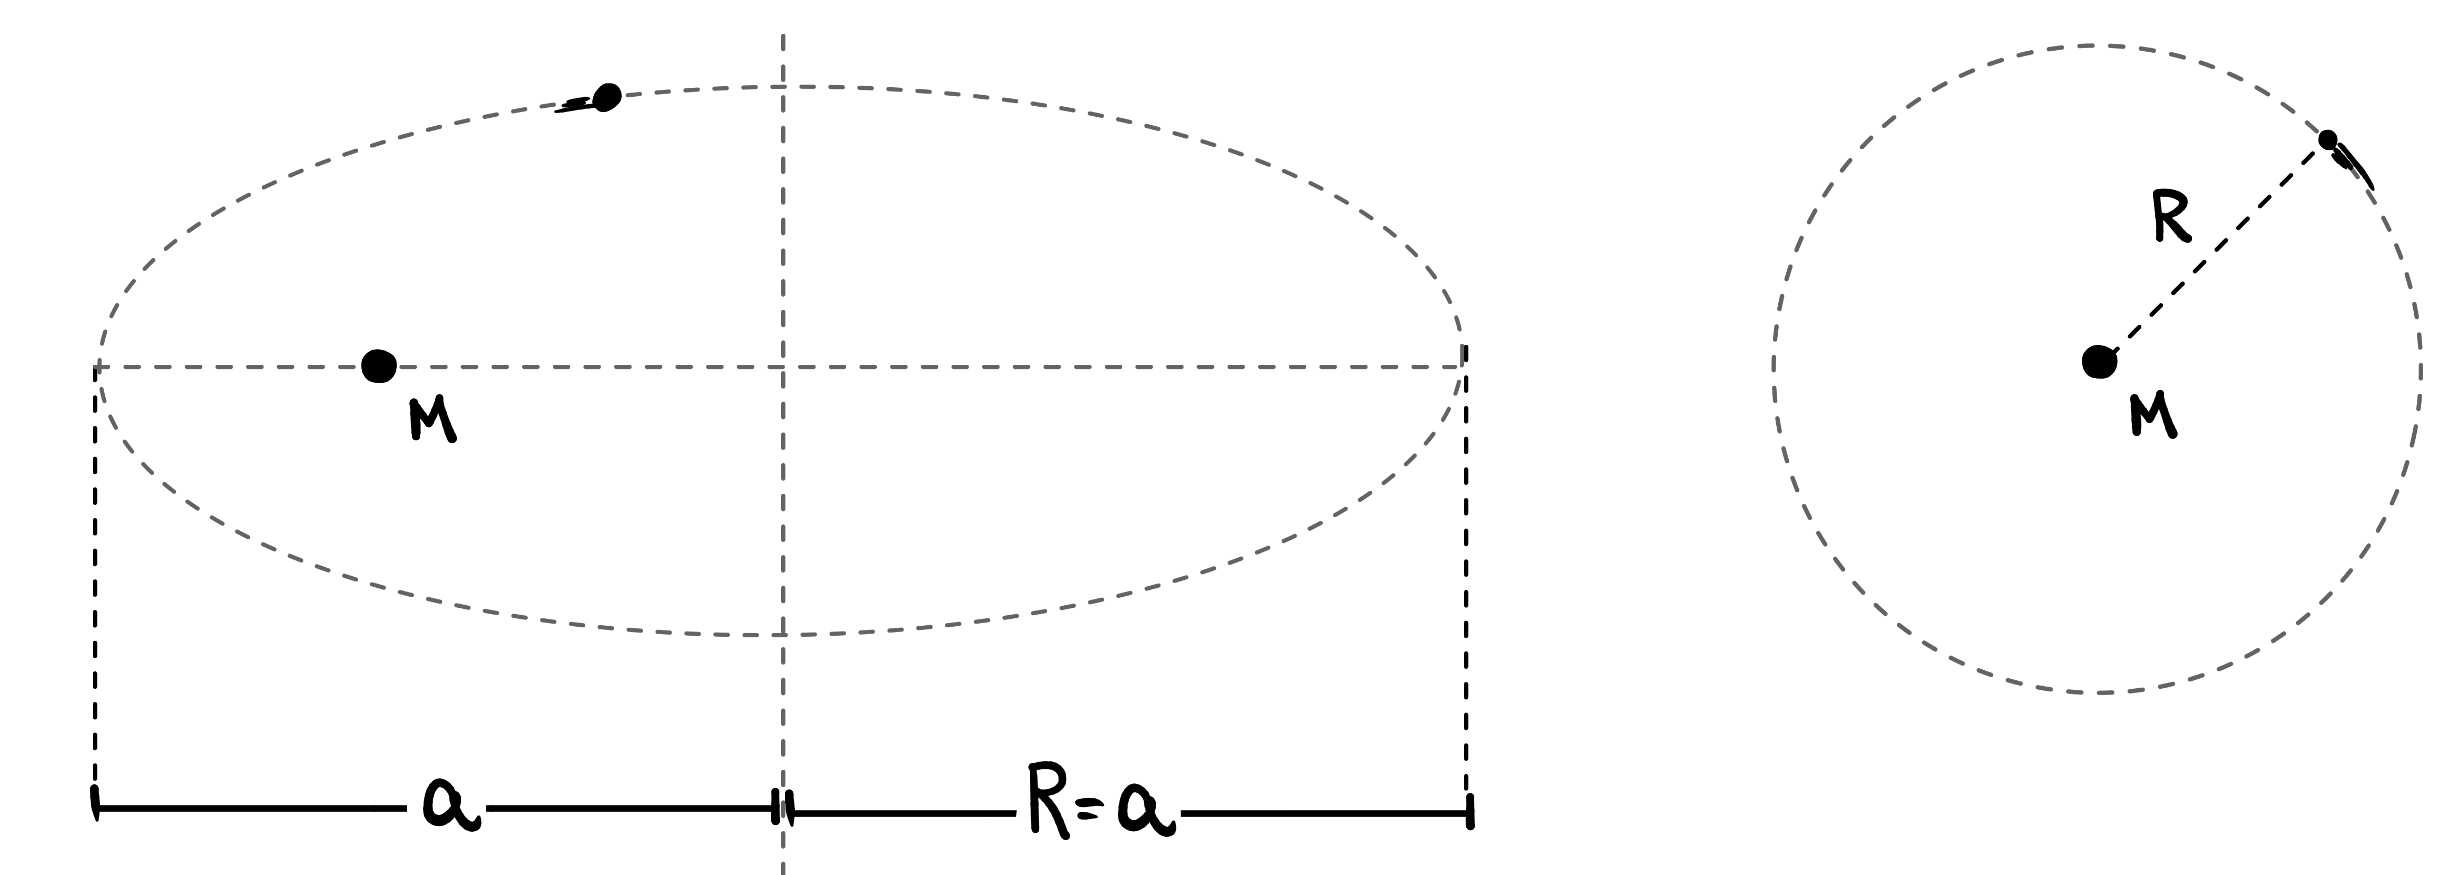
\includegraphics[width=0.7\linewidth]{imagensgravitacao/terceiraleikepler.png}
\captionof{figure}{Na terceira lei de Kepler, em caso de órbitas elípticas, o raio médio da órbita $R$ é igual ao semieixo maior $a$ da elipse.}
\label{fig_gravitacao_3ndkeplerslaw}
} 
\vspace{0.3cm}





Considere, por exemplo, o caso do sistema solar. Como a Terra e Marte estão orbitando em torno do mesmo astro\footnote{A Terra e Marte também interagem gravitacionalmente entre si, como veremos em breve. Contudo, como a massa do Sol é muito maior do que a daqueles dois planetas, a interação relevante para determinar o movimento deles se dá exclusivamente pela interação de cada um deles com o Sol.} -- o Sol --, podemos escrever que

$$\dfrac{T_T^2}{R_T^3} = \dfrac{T^2_M}{R^3_M},  $$

\noindent em que $T_T$ e $R_T$ representam o período de translação da Terra em torno do Sol e o raio da órbita da Terra em torno do Sol, o mesmo valendo para $T_M$ e $R_M$, que representam as respectivas grandezas para Marte.

Para entender de onde vem a Terceira Lei de Kepler, é preciso conhecer dois personagens
que, sem jamais terem trabalhado bem juntos em vida, produziram juntos, em morte, uma das
maiores descobertas da história da ciência.
 
O primeiro é \textit{Tycho Brahe} (1546--1601), astrônomo dinamarquês, famoso por usar
um nariz de prata --- o original fora perdido em um duelo acadêmico na juventude. Tycho
era, sem exagero, o maior observador astronômico do mundo pré-telescópio. Durante
décadas, a partir de seu observatório na ilha de Hven, ele mediu com precisão sem
precedentes as posições dos planetas no céu noite após noite, construindo o mais completo
e exato conjunto de dados astronômicos que a humanidade já havia reunido. Tycho sabia que
seus dados valiam ouro. Sabia também --- e isso o atormentava --- que não conseguia
construir com eles uma teoria coerente do sistema solar. Ele morreu em 1601 sem resolver
o quebra-cabeça, mas deixou os dados.
 
O segundo personagem é \textit{Johannes Kepler} (1571--1630), alemão, assistente de
Tycho nos últimos meses de vida do dinamarquês, e herdeiro legal dos dados. Kepler era o
oposto de Tycho: míope, fraco, propenso a doenças, filho de família pobre --- mas
matematicamente brilhante e com uma teimosia intelectual sobre-humana. Onde Tycho via
números, Kepler via padrões. Onde Tycho desistia, Kepler calculava de novo.
 
Kepler levou quase uma década debruçado sobre os dados de Tycho antes de anunciar suas
duas primeiras leis, em 1609: os planetas percorrem \textit{elipses} com o Sol em um dos
focos (Primeira Lei), e a linha que une o planeta ao Sol varre \textit{áreas iguais em
tempos iguais} (Segunda Lei). Foram dez anos de cálculos manuais. Dez anos. Em seguida,
Kepler passou mais uma década buscando uma terceira regularidade nos dados --- uma que
conectasse os períodos dos planetas às suas distâncias do Sol. E em 1619, no livro
\textit{Harmonices Mundi}, ele anunciou o que havia encontrado.\footnote{O título
\textit{Harmonices Mundi} --- ``As Harmonias do Mundo'' --- revela a motivação filosófica
de Kepler: ele acreditava que os planetas se moviam em proporções análogas às harmonias
musicais, que existia um padrão matemático por trás do movimento dos corpos do sistema solar.}
 
 
O leitor poderia indagar: como Kepler chegou à forma $T^2 \propto R^3$? Por que não
$T \propto R^2$, ou $T^3 \propto R^4$, ou qualquer outra combinação de potências?
 
A resposta é: porque ele tentou muitas combinações, e apenas uma funcionou para todos
os planetas simultaneamente. Kepler estava, em certo sentido, fazendo o que hoje
chamaríamos de ajuste de modelo --- procurando a relação matemática que melhor
descrevesse os dados. Mas ele não tinha computadores nem gráficos logarítmicos
automatizados. Tinha paciência, papel e uma convicção quase mística de que o cosmos
obedecia a proporções harmônicas.
 
A tabela abaixo mostra os dados que Kepler tinha à disposição, com os períodos e
distâncias médias dos seis planetas então conhecidos. Tomemos a Terra como referência,
com $T_\oplus = 1$\,ano e $R_\oplus = 1$\,UA (unidade astronômica):\footnote{A unidade
astronômica (UA) é definida como a distância média da Terra ao Sol, aproximadamente
$1{,}496 \cdot 10^{11}$\,m. É uma unidade conveniente para o sistema solar porque, ao
expressarmos distâncias em UA e períodos em anos terrestres, a constante $T^2/R^3$ vale
exatamente 1 para qualquer planeta do sistema solar.}
 


\vspace{0.8em}
\begin{center}
\setlength{\tabcolsep}{1.4em}
\renewcommand{\arraystretch}{1.45}
\setlength{\arrayrulewidth}{0.35pt}   % linhas internas finas
\begin{tabular}{@{\hspace{0.6em}}lrrrrr@{\hspace{0.6em}}}
  \hline
  \noalign{\vspace{2pt}}
  \textbf{Planeta} & $T$ (anos) & $R$ (UA) & $T^2$ & $R^3$ & $T^2/R^3$ \\
  \noalign{\vspace{2pt}}
  \hline
  \noalign{\vspace{1pt}}
  Mercúrio & $0{,}241$ & $0{,}387$ & $0{,}058$ & $0{,}058$ & $1{,}00$ \\ \hline
  Vênus    & $0{,}615$ & $0{,}723$ & $0{,}378$ & $0{,}378$ & $1{,}00$ \\ \hline
  Terra    & $1{,}000$ & $1{,}000$ & $1{,}000$ & $1{,}000$ & $1{,}00$ \\ \hline
  Marte    & $1{,}881$ & $1{,}524$ & $3{,}538$ & $3{,}540$ & $1{,}00$ \\ \hline
  Júpiter  & $11{,}86$ & $5{,}203$ & $140{,}7$ & $140{,}8$ & $1{,}00$ \\ \hline
  Saturno  & $29{,}46$ & $9{,}537$ & $868$     & $867$     & $1{,}00$ \\
  \noalign{\vspace{1pt}}
  \hline
\end{tabular}
\end{center}
\vspace{0.8em}



 
A razão $T^2/R^3$ é a mesma para todos os planetas. Não aproximadamente --- \textit{exatamente},
dentro dos erros de medição. O cosmos, de fato, obedecia a uma proporção. Kepler ficou
eufórico.
 
Mas note o que está \textit{ausente} nessa descoberta: Kepler não fazia a menor ideia de
\textit{por que} essa relação existia. Ele sabia \textit{que} $T^2/R^3$ era constante;
não sabia \textit{o quê} essa constante representava, nem o que a causava. Ela era, para
ele, uma harmonia cósmica --- bela, verdadeira e misteriosa. A explicação viria apenas
60 anos depois, com Newton.
 





\secgfe{Onde é usada}

 A Equação \eqref{eq_gravitacao_terceiraleikepler} é usada em contextos de gravitação, nos quais deseja-se descobrir o período de translação $T$ de um certo planeta, ou qual é a sua distância média $R$ até o astro em torno do qual ele está orbitando.



\secgfe{Erros comuns}

Os erros mais comuns quanto à aplicação da Equação \eqref{eq_gravitacao_terceiraleikepler} costumam ser em relação às unidades de medida. Considere, por exemplo, a situação em que se descobre um novo planeta $P$ do sistema solar, cujo período de translação em torno do Sol é de 36 meses terrestres. Deseja-se obter qual é a distância média $R_P$ de tal planeta ao Sol. Aplicando a Equação \eqref{eq_gravitacao_terceiraleikepler}, teremos

$$ \dfrac{T_T^2}{R_T^3} = \dfrac{T^2_P}{R^3_P},  $$

\noindent o que é válido, já que a Terra e tal planeta estão orbitando em torno do mesmo astro: o Sol. 

Agora, o valor do período de translação da Terra é conhecido, e a relação acima valerá quaisquer que sejam as unidades de medida usadas -- desde que se utilize a mesma dos dois lados. Logo, é fácil ver que usar o período em meses acarretará maiores dificuldades matemáticas: para a Terra teremos 12 meses, e para o planeta $P$ serão 36 meses. Tais números serão elevados ao quadrado e, posteriormente, teremos que extrair suas raízes cúbicas. Como os números são grandes, isso implicará dificuldades computacionais e, possivelmente, erros de cálculo ao longo do processo.

É mais fácil usar, portanto, o período em anos terrestres, de modo que $T_T = 1$ e $T_P=3$. Logo, a terceira lei de Kepler fica sendo:

$$ \dfrac{1^2}{R_T^3} = \dfrac{3^2}{R^3_P} \implies  R^3_P = 9  R_T^3 \implies R_P = \sqrt[3]{9} R_T \implies \boxed{R_P \approx 2.08R_T.}  $$

Ou seja, o raio da órbita $R_P$ de tal planeta em torno do Sol é aproximadamente o dobro do raio da órbita da Terra $R_T$ em torno do Sol.

Esse resultado teria sido obtido quaisquer que fossem as unidades de medida que escolhêssemos para o período: meses, dias, anos, horas, segundos ou qualquer outra. O importante é apenas que a mesma unidade que foi usada para um planeta seja usada para o outro. Desse modo, é sempre possível escolher uma unidade de medida em que os cálculos se simplifiquem, haja vista que os números ficarão menores.


\secgfe{Observações}



É importante notar que a Terceira Lei de Kepler tem um caráter cinemático: ela só explica como os planetas se movem, por exemplo, em torno do Sol. Eles se movem de tal modo que a razão entre os quadrados dos tempos que eles levam para completar uma órbita e os cubos dos raios de suas órbitas fornece sempre o mesmo valor. Perceba que esse é um fato cinemático: descreve-se um padrão matemático que o movimento deve respeitar, sem se preocupar com o que causa tais movimentos. 

A Lei da Gravitação Universal de Newton, expressa na Equação \eqref{eq_gravitacao_leigravitacaouniversal}, já é uma descrição dinâmica: ela diz qual é o tipo de força que gera o movimento que respeita a relação dada pela Equação \eqref{eq_gravitacao_terceiraleikepler}. Historicamente, as três leis de Kepler vieram antes de Newton, e foram leis obtidas a partir da análise de dados experimentais. Kepler notou, dadas as observações a respeito do movimento dos astros, que os planetas se movem de acordo com certos padrões, padrões esses que ele sintetizou em três leis sobre o movimento planetário.

A teoria newtoniana da gravitação veio a fim de explicar -- ou seja, trata-se de uma descrição dinâmica -- por que os planetas se moviam exatamente daquela forma. Ou seja, podemos entender a teoria da gravitação de Newton como uma teoria construída a partir das três leis de Kepler, de modo que, naturalmente, podemos demonstrar as três leis usando tal teoria, uma vez que as duas coisas contêm, de certo modo, o mesmo conteúdo físico.


% Conforme é discuto na construção da Equação \eqref{eq_gravitacao_leigravitacaouniversal}, a lei da Gravitação Universal é uma consequência da Terceira Lei de Kepler. Ou seja, podemos entender qual é o aspecto da força gravitacional com base na Terceira Lei de Kepler, ou, como fazemos lá, é possível demonstrar a Terceira Lei de Kepler com base na Lei da Gravitação Universal.


\vspace{0.3cm}

\begin{exemplo}[Nível I]\label{exemplo_gravitacao_keplerex01}

Dois satélites artificiais $S_1$ e $S_2$ orbitam a Terra com raios orbitais $r$ e $4r$, respectivamente (medidos a partir do centro da Terra). Sabe-se que $S_1$ tem período de 90 minutos. Qual é o período de $S_2$, em minutos?


\resolucao

Como os dois satélites estão orbitando o mesmo corpo (Terra), vale a terceira lei de Kepler, isto é:



$$ \dfrac{T_1^2}{R_1^3} = \dfrac{T^2_2}{R^3_2} \implies  \dfrac{T_1^2}{r^3} = \dfrac{T^2_2}{(4r)^3} \implies T_2^2 =  4^3 T_1^2 = 2^6 T_1^2,$$


\noindent de onde segue que $T_2 = 2^3 T_1 = 8T_1.$ Como o período de translação do satélite $S_1$ é $T_1 = 90$ min, segue que 

$$ \boxed{T_2 = 8 T_1 = 8 \cdot 90 = 720 \text{ minutos.}}$$

Observe que, para evitar de elevar 90 ao quadrado e depois extrair sua raiz cúbica, carregamos o período $T_1$ de $S_1$ de forma literal para, apenas no último passo, substituirmos o seu valor.

\end{exemplo}



\vspace{0.3cm}



\begin{exemplo}[Nível II]\label{exemplo_gravitacao_keplerex02}

Um cometa altamente excêntrico tem período orbital de 27 anos em torno do Sol. Usando a Terra como referência, qual é o valor do semieixo maior de sua órbita, em UA?

Considere que 1 UA (Unidade Astronômica) é igual à distância média entre a Terra e o Sol.


\resolucao

Assumindo que tal cometa está orbitando o Sol, podemos escrever que 

$$ \dfrac{T_T^2}{R_T^3} = \dfrac{T^2_C}{R^3_C} \implies  \dfrac{1^2}{(1\text{ UA)}^3} = \dfrac{27^2}{R^3_C} \implies R_C^3=  3^6 (1\text{ UA)}^3,$$

\noindent de onde segue que $R_C= 9 \text{ UA.}$

\end{exemplo}



\vspace{0.3cm}



\begin{exemplo}[Nível III - Órbita de Transferência de Hohmann]\label{exemplo_gravitacao_keplerex03}


Para elevar um satélite de uma órbita circular de raio $r_A$ para uma
órbita circular maior de raio $r_B$, engenheiros utilizam a
\textit{órbita de transferência de Hohmann}: um único impulso lança o
satélite numa elipse que tangencia internamente as duas órbitas,
como mostra a figura abaixo.

\begin{center}
\begin{tikzpicture}[scale=0.6, line cap=round, line join=round]

    % Parâmetros
    \def\rA{1.55}
    \def\rB{3.35}
    \pgfmathsetmacro{\a}{(\rA+\rB)/2}      % semi-eixo maior
    \pgfmathsetmacro{\c}{(\rB-\rA)/2}      % distância centro-foco
    \pgfmathsetmacro{\b}{sqrt(\a*\a-\c*\c)}% semi-eixo menor

    % Terra no foco
    \coordinate (O) at (0,0);

    % Centro da elipse
    \coordinate (C) at (-\c,0);

    % Pontos extremos
    \coordinate (A) at (\rA,0);
    \coordinate (B) at (-\rB,0);

    % Órbitas circulares
    \draw (O) circle (\rA);
    \draw (O) circle (\rB);

    % Elipse de transferência
    \draw (C) ellipse ({\a} and {\b});

    % Diâmetro horizontal
    \draw (B) -- (A);

    % Terra
    \fill (O) circle (1.1pt);

    % Vetores velocidade
    % \draw[->] (A) -- ++(0,0.95);
    % \node[right] at ($(A)+(0,0.95)$) {$v_A$};

    % \draw[->] (B) -- ++(0,-0.95);
    % \node[left] at ($(B)+(0,-0.95)$) {$v_B$};

    % Rótulos dos pontos
    \node[right] at (A) {$A$};
    \node[left] at (B) {$B$};

    % Rótulo r_A
    \node[below] at ($(O)!0.57!(A)$) {$r_A$};

    % Rótulo r_B deslocado para não cruzar a órbita interna
    \node[above] at ($(B)!0.23!(O)$) {$r_B$};

\end{tikzpicture}
\end{center}

O corpo central (Terra) está no ponto focal da elipse. O satélite parte
do ponto~$A$ — onde a elipse toca a órbita interna (\textit{perigeu})
— e chega ao ponto~$B$ — onde a elipse toca a órbita externa
(\textit{apogeu}) — percorrendo exatamente metade da elipse.

\medskip

Sabendo que $r_B = 3\,r_A$ e que o período do satélite na órbita
interna é $T_A$, qual é o tempo de viagem de $A$ até $B$?


\medskip

\begin{enumerate}
  \item [a)] $\dfrac{1}{2}T_A$
  \item [b)]$\dfrac{\sqrt{3}}{2}T_A.$
  \item [c)]$\sqrt{2}T_A.$
  \item [d)]$2\sqrt{2}T_A.$ 
  \item [e)]$3\sqrt{3}T_A.$ 
\end{enumerate}

\resolucao

A elipse tangencia as duas órbitas circulares: seu periélio está em
$r_A$ e seu afélio em $r_B = 3r_A$. Por definição geométrica da elipse,
o semieixo maior $a$ é a semissoma dos raios extremos:
%
\begin{equation}
  a \;=\; \frac{r_A + r_B}{2} \;=\; \frac{r_A + 3r_A}{2} \;=\; 2r_A. \nonumber
  \label{eq:semieixo-hoh}
\end{equation}


Tanto a órbita interna quanto a elipse de transferência têm o mesmo
corpo central, portanto a constante $T^2/R^3$ é a mesma para ambas.
Usando a órbita interna como referência:
%
\begin{equation}
  \frac{T_{\text{trans}}^2}{T_A^2}
  \;=\; \frac{a^3}{r_A^3}
  \;=\; \frac{(2r_A)^3}{r_A^3}
  \;=\; 8
  \;\;\Longrightarrow\;\;
  T_{\text{trans}} \;=\; 2\sqrt{2}\;T_A. \nonumber
  \label{eq:periodo-hoh}
\end{equation}

O satélite percorre apenas o semiarco da elipse — do periélio~$A$
ao afélio~$B$ —, o que corresponde a exatamente metade do período
de transferência:
%
\begin{equation}
  \boxed{t_{A \to B} 
  \;=\; \frac{T_{\text{trans}}}{2}
  \;=\; \frac{2\sqrt{2}}{2}\,T_A
  \;=\; \sqrt{2}\;T_A \implies \text{ letra C.}} \nonumber
  \label{eq:tempo-hoh}
\end{equation}



\end{exemplo}










\begin{secnivel}[Lei da Gravitação Universal]{I}{Lei da Gravitação Universal}
  
  \eqLdois{exp}{eq_gravitacao_leigravitacaouniversal}{F = G\dfrac{Mm}{r^2}}

\end{secnivel}




\secgfe{De onde vem}

Imagine que você está em 1666, numa fazenda em Woolsthorpe, na
Inglaterra. A peste bubônica fechou a Universidade de Cambridge -- e
Isaac Newton, com 23 anos, foi mandado para casa. Pandemia, lockdown. Não havia muito para
fazer. E foi exatamente daí que nasceu uma das maiores ideias da história da humanidade.


%Transportar esse trecho para a parte da velocidade orbital!!!!

% A história da maçã é, provavelmente, um mito. Mas a pergunta que Newton
% se fez é real e poderosa: \textit{se a Terra puxa a maçã para baixo,
% será que ela também puxa a Lua?} E se puxa, por que a Lua não cai?

% Ela cai. Só que ela também se move para o lado --- e quando você combina
% queda com movimento lateral, o resultado é uma órbita. Newton percebeu
% isso com uma elegância rara: a Lua está em queda livre permanente em
% torno da Terra. O que muda em relação à maçã não é a natureza da força
% --- é a distância.

% Newton sabia, graças aos dados astronômicos de Tycho Brahe e às leis de
% Kepler (especialmente a Terceira Lei, $T^2 \propto R^3$), que os
% planetas mais distantes do Sol se movem mais devagar. Usando a expressão
% da aceleração centrípeta $a_c = v^2/R$, e a relação de Kepler para
% deduzir como a velocidade orbital varia com a distância, ele chegou a
% uma conclusão: \textbf{a força gravitacional entre dois corpos diminui
% com o quadrado da distância entre eles}. Essa dependência em $1/r^2$
% ficou conhecida como a ``lei do inverso do quadrado'' --- e ela aparece
% com surpreendente frequência na natureza (como veremos futuramente na
% lei de Coulomb para forças elétricas).

% Mas a distância não é o único fator. Intuitivamente --- e confirmado
% pelas leis de Newton --- a força também deve depender das massas
% envolvidas. Pela Terceira Lei, a força que a Terra exerce sobre a maçã
% é igual e oposta à que a maçã exerce sobre a Terra. Logo, a força deve
% ser proporcional às duas massas simultaneamente.

% A constante $G$ é o fator de proporcionalidade universal: ela foi
% medida experimentalmente, pela primeira vez, por Henry Cavendish em
% 1798 --- mais de cem anos depois da morte de Newton --- com um
% experimento engenhoso usando uma balança de torção com esferas de
% chumbo. 

% Assim nasce a lei:

% \[
%     F = G\frac{m_1 m_2}{r^2}
% \]

% Não é uma equação derivada de princípios mais fundamentais --- ela foi
% induzida da observação da natureza e consagrada por sua capacidade
% preditiva extraordinária.

% Podemos, contudo, construir e ver como surge a dependência do inverso do quadrado da distância, partindo da Terceira Lei de Kepler, a Equação \eqref{eq_gravitacao_terceiraleikepler}. Considere, para tanto, um planeta de massa $m$, que está em uma órbita circular de raio $r$, em torno de uma estrela de massa $M$. A Figura \ref{} ilustra tal situação.

% FIGURA


% Sabemos que a força gravitacional atuará como resultante centrípeta, isto é

% $$  F_G = F_{\text{R}_{CPT}}  \implies  F_G =\dfrac{mv^2}{r}. $$

% O que queremos aqui é justamente estudar e entender o aspecto da força gravitacional $F_G.$ Sendo o movimento circular uniforme, o valor da velocidade será constante, de modo que podemos escrever que

% $$ v= \dfrac{d}{t} = \dfrac{2 \pi r}{T} \implies v^2 = \dfrac{4 \pi^2 r^2}{T^2},$$

% \noindent o que, na relação anterior, fornece

% $$ F_G =\dfrac{mv^2}{r} = \dfrac{m}{r} \cdot \dfrac{4 \pi^2 r^2}{T^2},$$

% \noindent e, pela Terceira Lei de Kepler, como $T^2 = k r^3,$ teremos

% $$ F_G =\dfrac{m}{r} \cdot \dfrac{4 \pi^2 r^2}{kr^3} \implies F_G = \left(\dfrac{4 \pi^2 m}{k} \right)\dfrac{1}{r^2},$$

% \noindent ou seja, sendo $\pi, k$ e $m$ valores definidos, vemos que a força de atração gravitacional $F_G$ é inversamente proporcional ao quadrado da distância $r$ entre os corpos.


% Reescrever a secção, partindo do fio a ser costurado:
% 1) Porque deve haver uma força de atração
% 2) Sendo a gravidade uma força atrativa (centripeta), como deve ser seu aspecto?
% 3) Constrói-se a dependência em r^2, e sobre a massa m na jogada.
% 4) Pela terceira lei de newton, por simetria, a força deve depender de M, de modo que ela depende, portanto, do produto das massas
% 5) F \prop Mm/r^2, de modo que tem-se a lei da gravitação universal.


A construção da Lei da Gravitação Universal se deu mais ou menos de acordo com esses passos:

\begin{enumerate}
    \item [(i)] A força que mantém os planetas em órbita é a mesma que faz a maçã cair.


    Que os objetos na superfície da Terra eram atraídos em direção ao chão já era de conhecimento da humanidade muito antes de Newton. A genialidade deste esteve em perceber que a mesma força que faz a maçã cair é a que mantém os planetas em órbita, e que o próprio movimento orbital é, em certa medida, uma queda. A Figura \ref{fig_gravitacao_orbitar=cair1} mostra essa composição de movimentos: um corpo tende a se mover, como diz a Primeira Lei de Newton, com velocidade constante ao longo de uma linha reta, exatamente na direção em que aponta a sua velocidade -- por inércia. Contudo, devido à ação gravitacional do planeta, esse corpo terá sua trajetória perturbada, por ser atraído em direção ao planeta. 



\vspace{0.3cm}
{
\centering
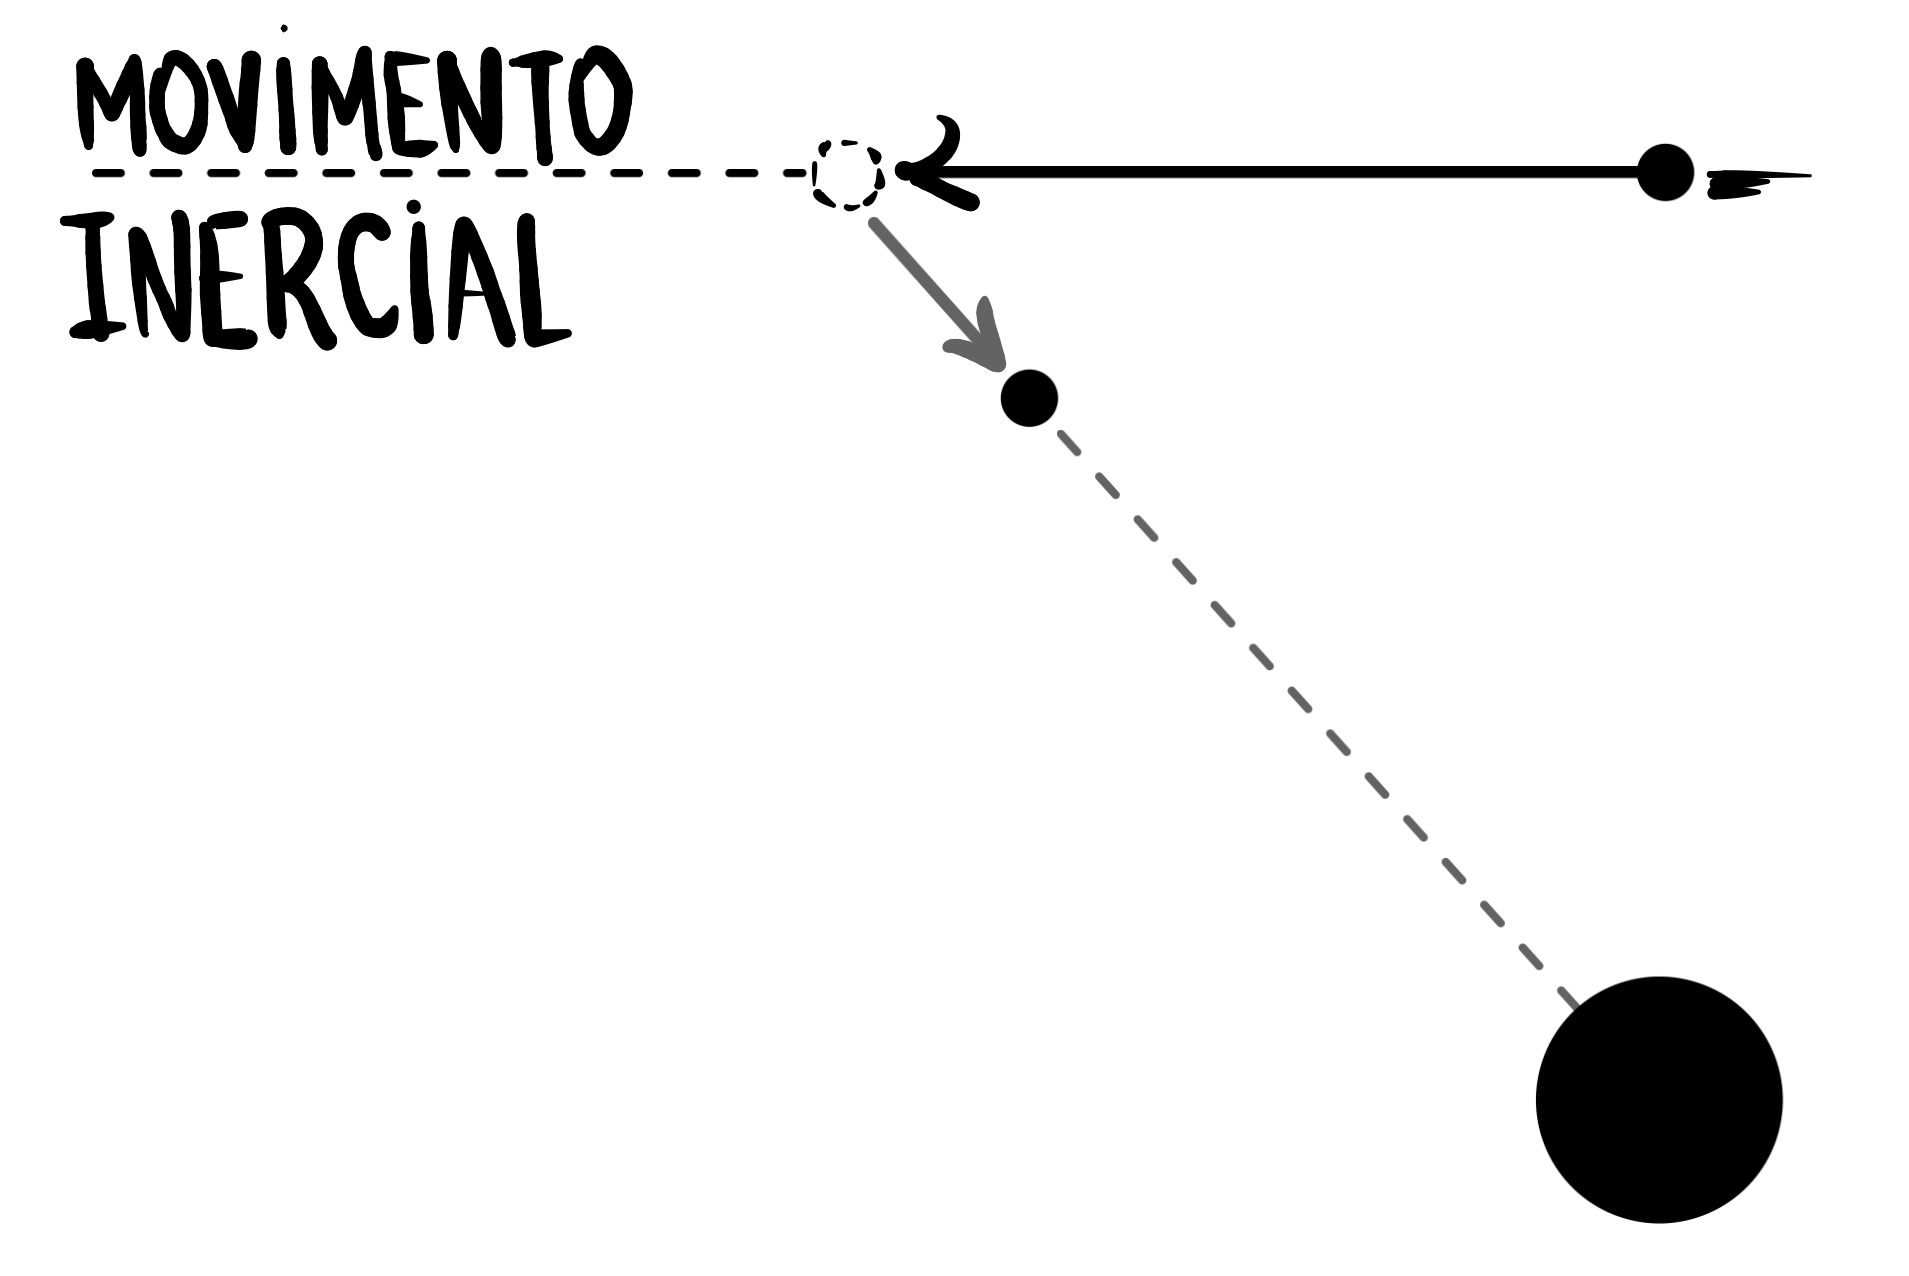
\includegraphics[width=0.4\linewidth]{imagensgravitacao/orbitar=cair1.png}
\captionof{figure}{O movimento orbital é a composição de dois efeitos: a tendência de sair pela direção da tangente, na direção em que aponta a velocidade, em linha reta; com a atração em direção ao centro.}
\label{fig_gravitacao_orbitar=cair1}
} 
\vspace{0.3cm}


Desse modo, podemos enxergar o movimento de tal satélite como sendo, em cada instante, uma composição desses dois movimentos: a tendência de sair pela tangente, por inércia, na direção em que aponta a sua velocidade (caso não houvesse nenhuma força o corpo simplesmente se moveria em MRU ao longo dessa direção), com uma queda em direção ao planeta, proporcionada pela força de atração gravitacional. Compondo mais alguns trechos desse movimento, como mostra a Figura \ref{fig_gravitacao_orbitar=cair2}, conseguimos construir uma visão melhor dessa composição -- a tendência de sair pela tangente com uma pequena queda em direção à linha que une os corpos.

\vspace{0.3cm}
{
\centering
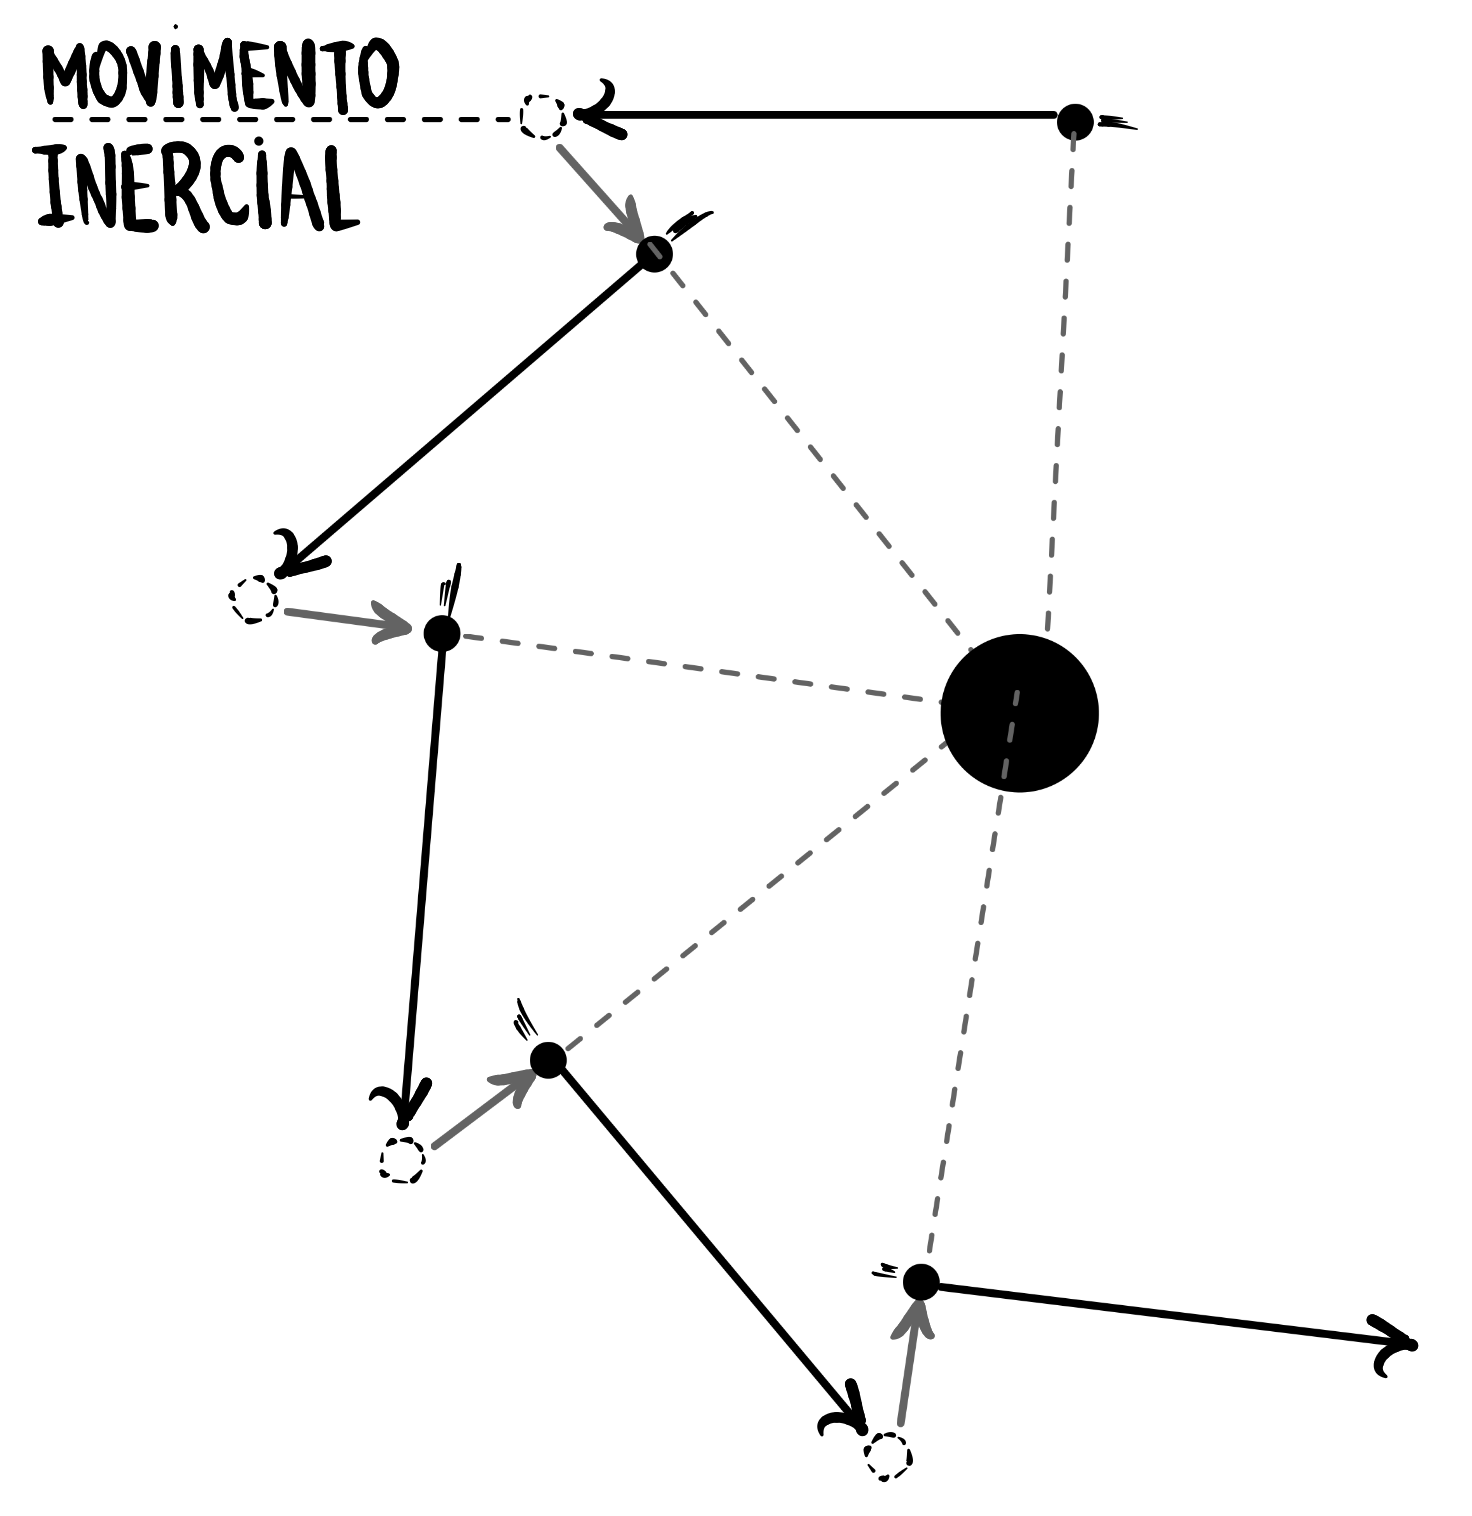
\includegraphics[width=0.5\linewidth]{imagensgravitacao/orbitar=cair3.png}
\captionof{figure}{A composição da tendência de sair pela tangente -- por inércia, em MRU -- com uma queda em direção ao centro.}
\label{fig_gravitacao_orbitar=cair2}
} 
\vspace{0.3cm}




Por fim, a Figura \ref{fig_gravitacao_orbitar=cair3} mostra o ciclo completo: se houver uma harmonia exata -- que será computada pela Equação \eqref{eq_gravitacao_velocidadeorbital} -- entre a velocidade do planeta (que representa sua tendência de sair pela tangente e se mover em linha reta) com o campo gravitacional do planeta central (que representa a tendência do primeiro planeta cair e colidir contra o segundo) é possível construir exatamente um movimento orbital.

\vspace{0.3cm}
{
\centering
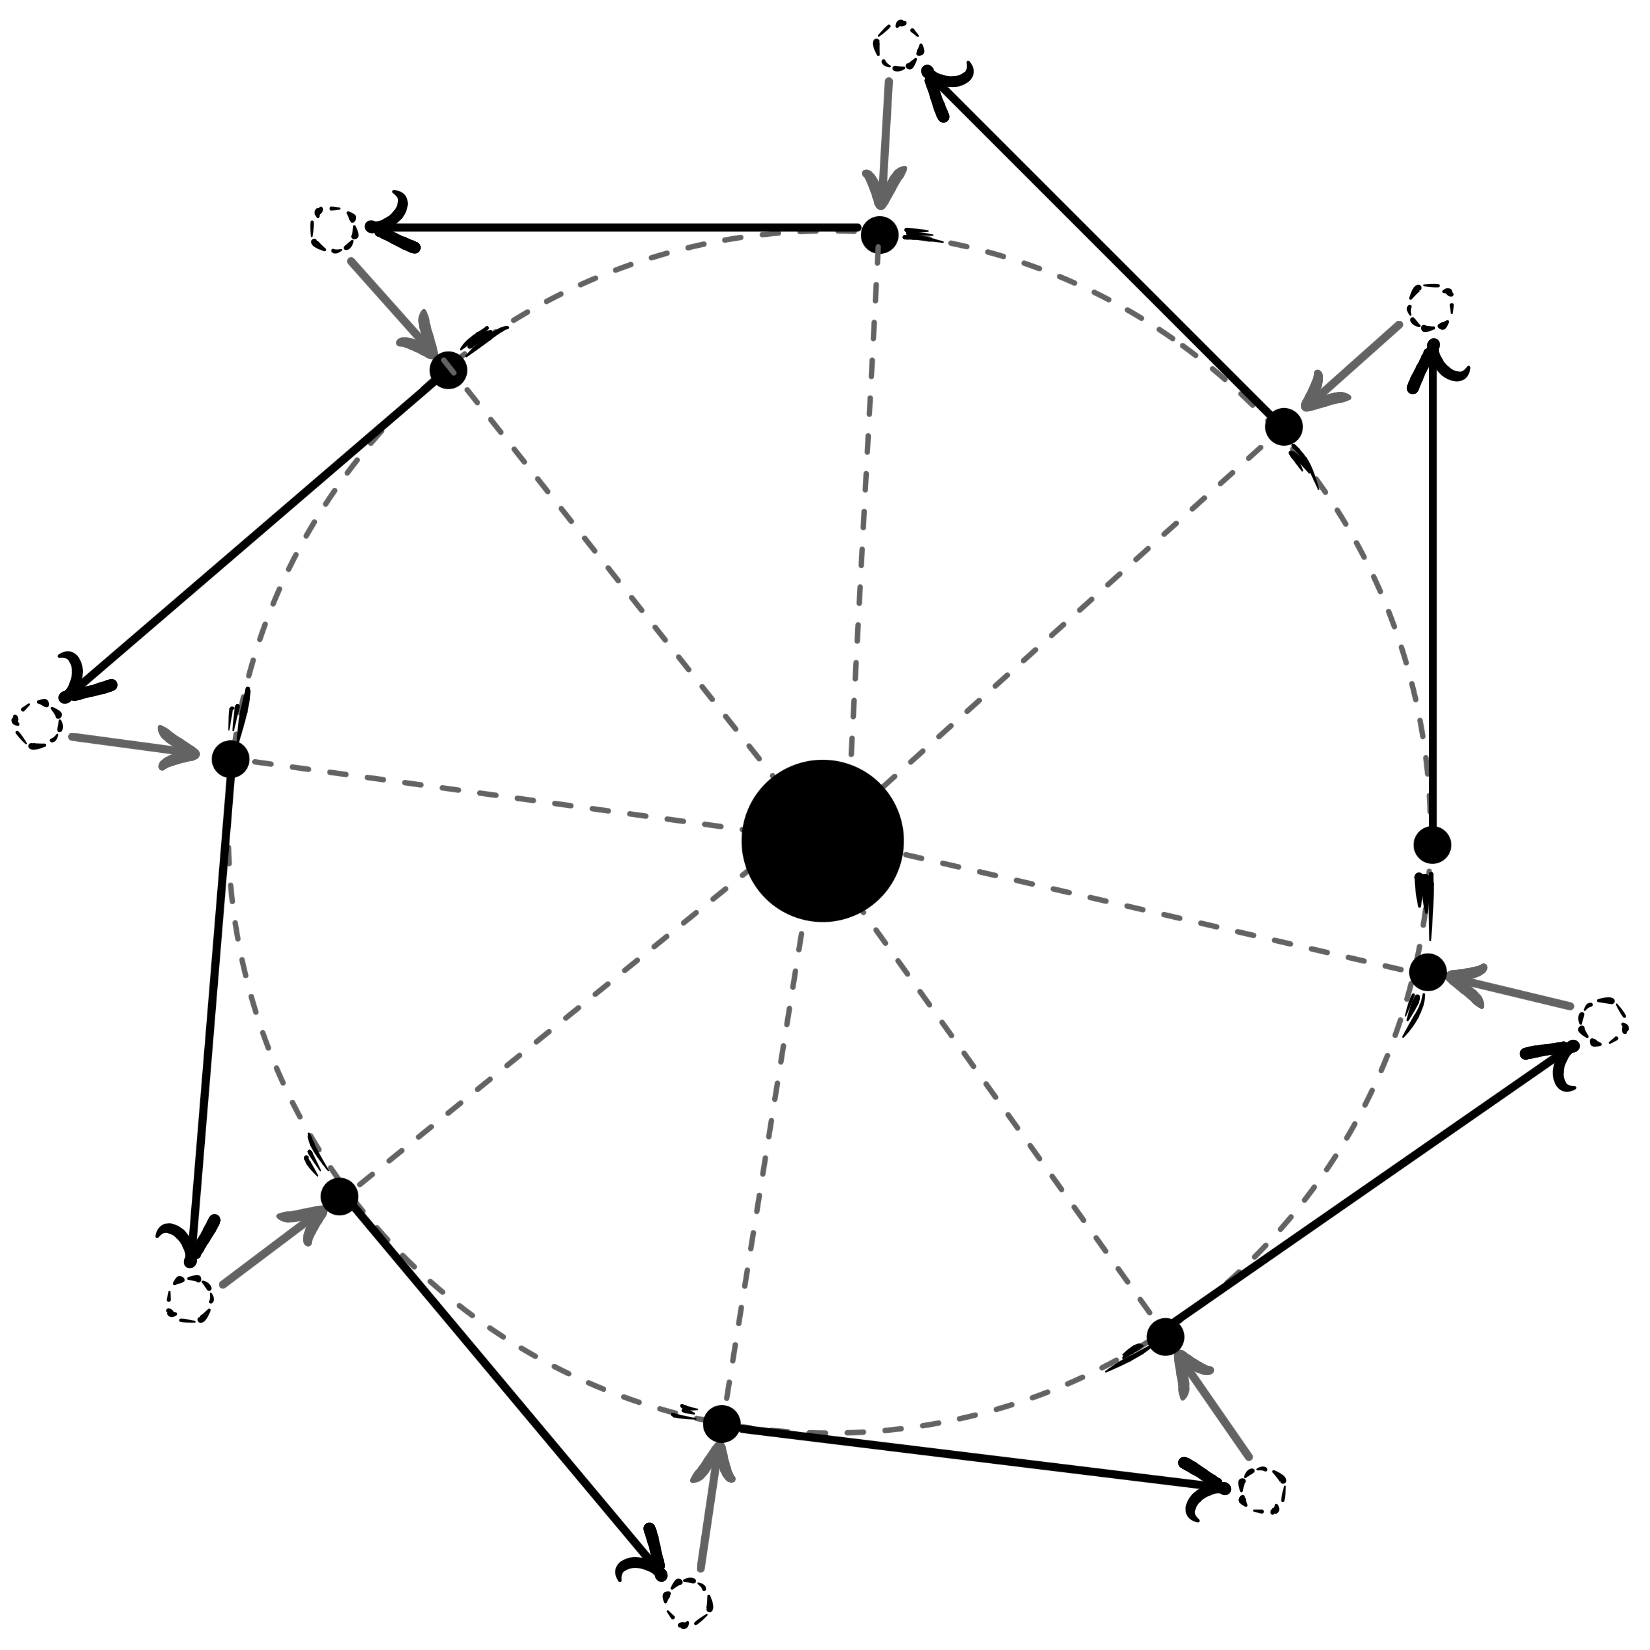
\includegraphics[width=0.5\linewidth]{imagensgravitacao/orbitar=cair2.png}
\captionof{figure}{O movimento orbital é uma queda.}
\label{fig_gravitacao_orbitar=cair3}
} 
\vspace{0.3cm}
    
Assim, a mesma força que atrai a maçã em direção ao centro da Terra e faz ela cair -- sua força peso -- é a que mantém os planetas em órbita -- a força de atração gravitacional. A queda livre e o movimento orbital são duas manifestações de um mesmo fenômeno.
    

    \item [(ii)] Sendo a gravidade uma força atrativa, a Terceira Lei de Kepler exige que essa força dependa do inverso do quadrado da distância, ou seja, $F \propto 1/r^2$.

Considere um planeta de massa $m$, que está em uma órbita circular de raio $r$, em torno de uma estrela de massa $M$. A Figura \ref{fig_gravitacao_deducaogravitacao} ilustra tal situação.


\vspace{0.3cm}
{
\centering
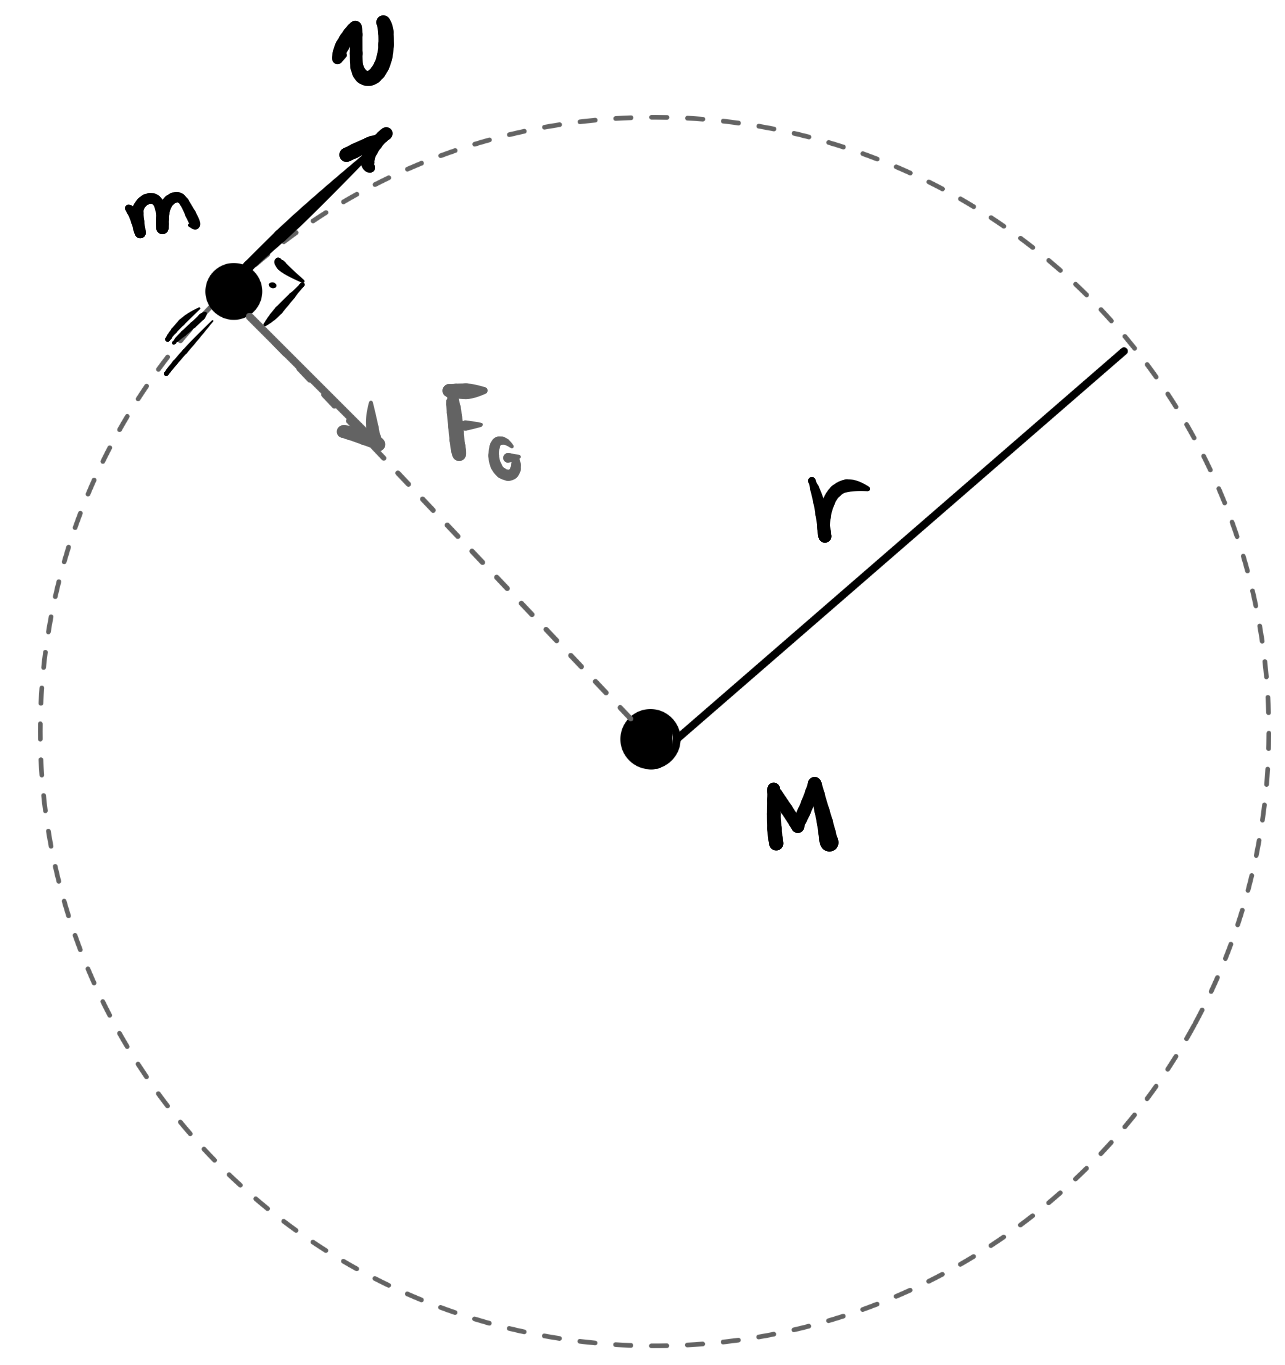
\includegraphics[width=0.3\linewidth]{imagensgravitacao/gravitacaodeducao.png}
\captionof{figure}{A força $F_G$ que mantém o planeta em órbita deve ser atrativa, atuando como resultante centrípeta.}
\label{fig_gravitacao_deducaogravitacao}
} 
\vspace{0.3cm}


Sabemos que a força gravitacional, que é atrativa, atuará como resultante centrípeta, isto é

$$  F_G = F_{\text{R}_{CPT}}  \implies  F_G =\dfrac{mv^2}{r}. $$

O que queremos aqui é justamente estudar e entender o aspecto da força gravitacional $F_G.$ Sendo o movimento circular uniforme, o valor da velocidade será constante, de modo que podemos escrever que

$$ v= \dfrac{d}{t} = \dfrac{2 \pi r}{T} \implies v^2 = \dfrac{4 \pi^2 r^2}{T^2},$$

\noindent o que, na relação anterior, fornece

$$ F_G =\dfrac{mv^2}{r} = \dfrac{m}{r} \cdot \dfrac{4 \pi^2 r^2}{T^2},$$

\noindent e, pela Terceira Lei de Kepler, como $T^2 = k r^3,$ teremos

$$ F_G =\dfrac{m}{r} \cdot \dfrac{4 \pi^2 r^2}{kr^3} \implies F_G = \left(\dfrac{4 \pi^2 m}{k} \right)\dfrac{1}{r^2},$$

\noindent ou seja, sendo $\pi, k$ e $m$ valores definidos, vemos que a força de atração gravitacional $F_G$ deve ser inversamente proporcional ao quadrado da distância $r$ entre os corpos, a fim de ser compatível com a Terceira Lei de Kepler.
     

    \item[(iii)] Pela Terceira Lei de Newton, a força deve depender do produto das massas.

    Ora, se a força que atua no planeta $m$, devido à ação de $M$, é proporcional à sua massa $m,$ como mostra a expressão anterior, pela Terceira Lei de Newton sabemos que o planeta de massa $m$ faz uma força igual e contrária em $M$. Contudo, por simetria, a força em $M$ deve, também, ser proporcional à sua própria massa $M$. 

    Desse modo, concluímos que a força gravitacional $F_G$ deve ser proporcional ao produto das massas dos corpos que interagem, isto é:

    $$ F \propto (Mm).$$

    \item [(iv)] Por fim, basta uma constante para ajustar a equação.

    Até então concluímos que 

    $$ F_G \propto \dfrac{Mm}{r^2},$$

    \noindent de modo que basta inserirmos uma constante para que tal relação de proporcionalidade se torne uma equação. A constante em questão é a constante de gravitação universal $G$, que produz, por fim, a Equação \eqref{eq_gravitacao_leigravitacaouniversal}.

    Newton publicou sua Lei da Gravitação Universal em 1687, mas ele mesmo morreu sem saber exatamente qual seria o valor da constante $G$. Veja que determinar o valor de tal constante não é exatamente simples. Para medir $G$, você precisaria medir a força gravitacional entre dois objetos em um laboratório. Conhecendo a força, suas massas e sua distância, a Equação \eqref{eq_gravitacao_leigravitacaouniversal} nos permitiria obter o valor de $G:$

    $$ G = \dfrac{F_G \cdot r^2}{Mm}.$$
    
    
    Mas a gravidade é absurdamente fraca, conforme pontuaremos posteriormente -- uma pedra não é atraída para outra pedra ao lado dela de forma perceptível. Só planetas e estrelas têm massa suficiente para exercer forças que sentimos.

A solução veio de um inglês excêntrico e recluso chamado Henry Cavendish. Ele adaptou um aparato já existente -- uma balança de torção -- e conduziu um experimento de precisão extraordinária em seu laboratório particular. O dispositivo consistia em uma barra horizontal suspensa por um fio fino, com duas pequenas esferas de chumbo nas extremidades. Cavendish então aproximava duas grandes esferas de chumbo dessas pequenas, como mostra a Figura \ref{fig_gravitacao_balancatorcao}.


\vspace{0.3cm}
{
\centering
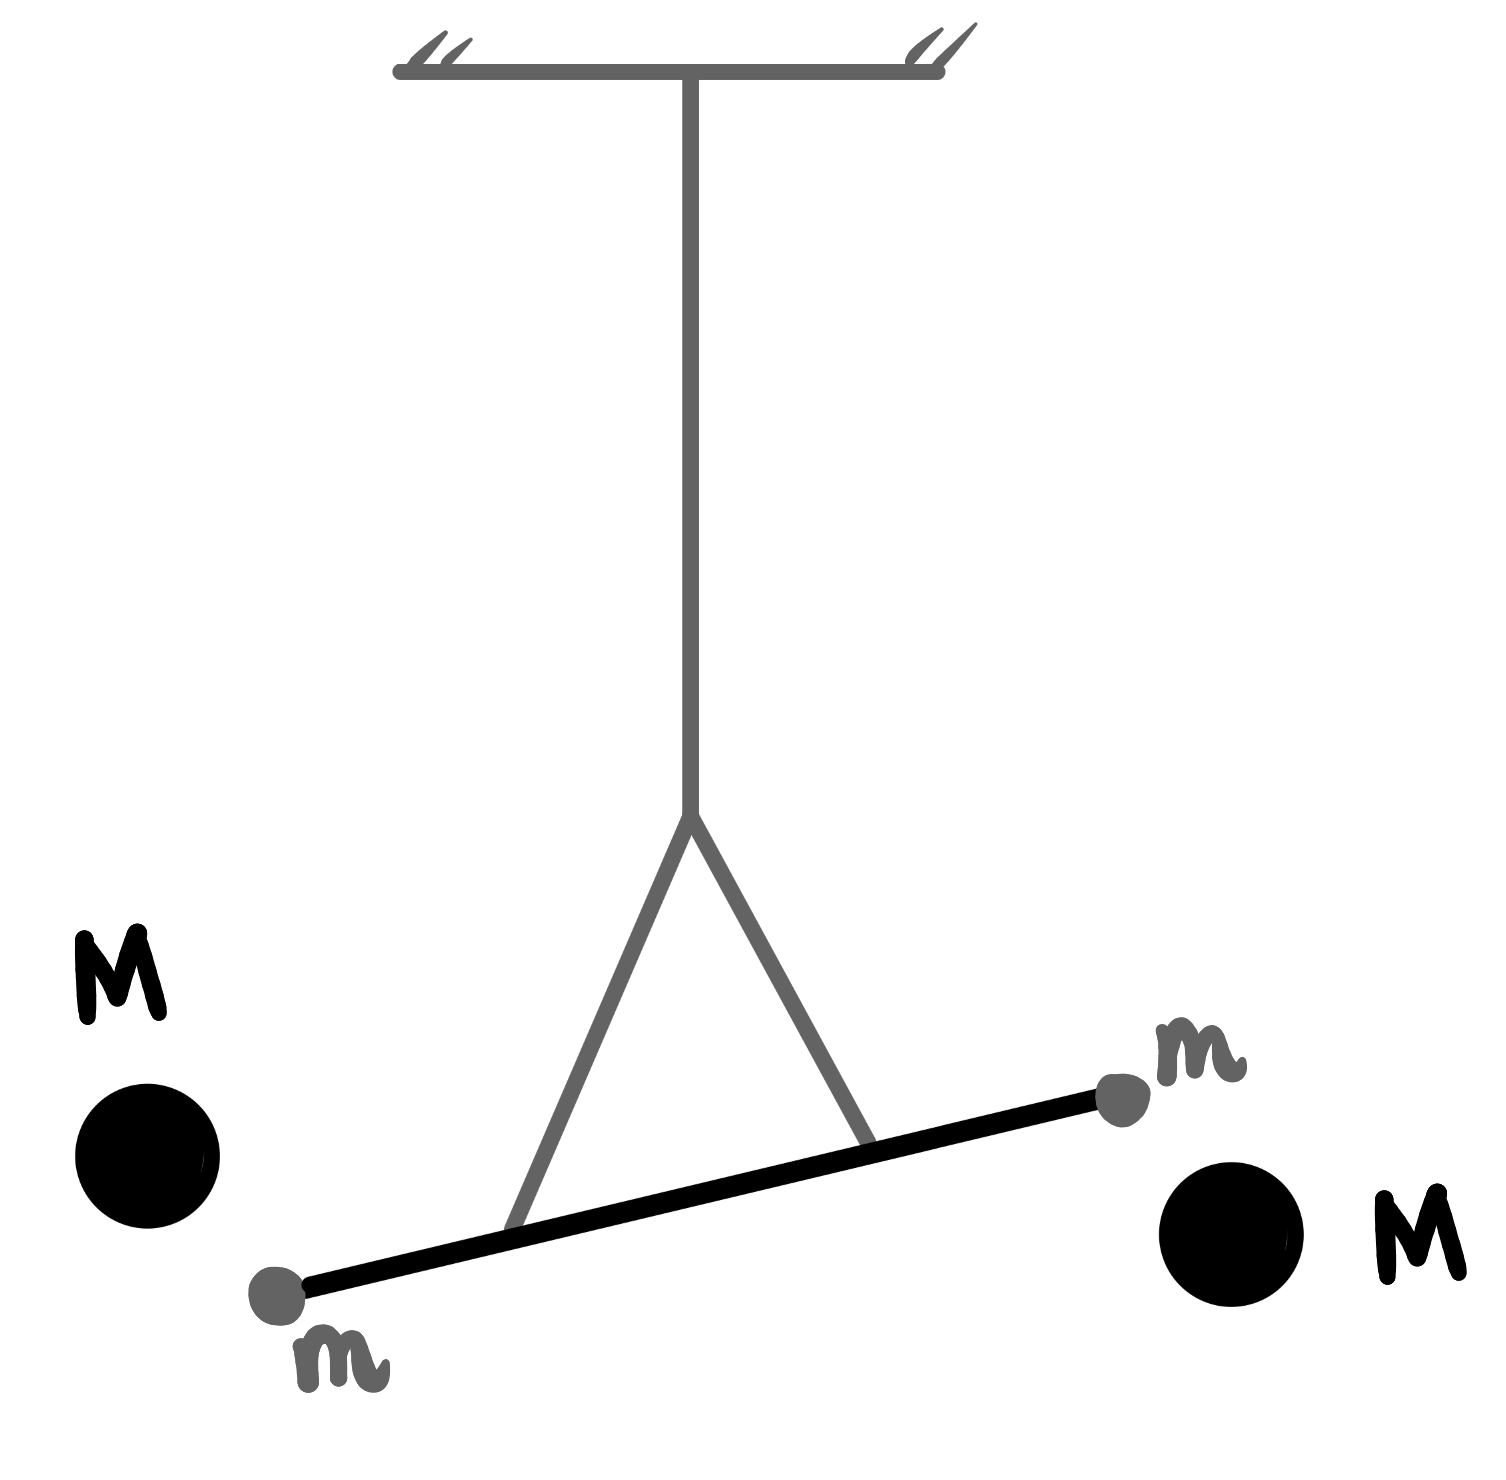
\includegraphics[width=0.3\linewidth]{imagensgravitacao/balancatorcao.png}
\captionof{figure}{Esboço da balança de torção usada por Cavendish.}
\label{fig_gravitacao_balancatorcao}
} 
\vspace{0.3cm}



A atração gravitacional, por menor que fosse, torcia levemente o fio. Medindo o ângulo de torção -- usando um telescópio de fora do cômodo para não perturbar o ar -- ele calculava a força. O experimento durou meses. Cavendish se recusava a entrar no cômodo durante as medições, tamanha era a sensibilidade do aparato. Qualquer corrente de ar ou variação de temperatura arruinava tudo.
O resultado? Ele obteve um valor para G de aproximadamente $6.74 × 10^{-11} \text{N} \cdot \text{m}^2/\text{kg}^2$ -- notavelmente próximo do valor aceito hoje, que é $6.674 × 10^{-11} \text{N} \cdot \text{m}^2/\text{kg}^2$.\footnote{Curiosamente, Cavendish não pensava que estava ``medindo $G$''. Para ele, o objetivo era ``pesar a Terra'' -- determinar a densidade média do nosso planeta. $G$ era um subproduto do cálculo. A mentalidade da época ainda não havia abstraído a constante como uma quantidade fundamental independente.}

\end{enumerate}









\secgfe{Onde é usada}

A Equação \eqref{eq_gravitacao_leigravitacaouniversal} nos diz como calcular a força $F$ de interação gravitacional entre duas massas $M$ e $m,$ separadas por uma distância $r$. 

Em praticamente todo contexto que envolva gravitação, tal equação será aplicada. As próximas quatro ou cinco equações que estudaremos na sequência serão, em certa medida, apenas uma aplicação da Equação \eqref{eq_gravitacao_leigravitacaouniversal}. Desde o cálculo de órbitas, de qual é a velocidade com que um satélite deve ser lançado até o cálculo de energias que envolvam a gravidade, todos eles passarão, em alguma parte, pelo uso da Equação \eqref{eq_gravitacao_leigravitacaouniversal}.




\secgfe{Erros comuns}

Os erros mais comuns se dividem em dois tipos:

\begin{enumerate}
    \item [(i)] Confundir $r$ com a altura em relação à superfície.

O erro clássico: um problema informa que um satélite orbita a Terra a 400\,km de
altura. O leitor usa $r= 400$ km na Equação \eqref{eq_gravitacao_leigravitacaouniversal}. O valor de $r$ na Lei
da Gravitação é a \textbf{distância entre os centros de massa} dos dois
corpos — não a altitude acima da superfície. Para um satélite em órbita terrestre, o correto é usar $r = R + h = 6.400 + 400  = 6.800$ km, em que $R=6.400$ km é o raio da Terra, como mostra a Figura \ref{fig_gravitacao_leigravitacaouniversal}. Usar apenas $h$ subestima brutalmente a distância real e produz um
resultado errado.

\vspace{0.3cm}
{
\centering
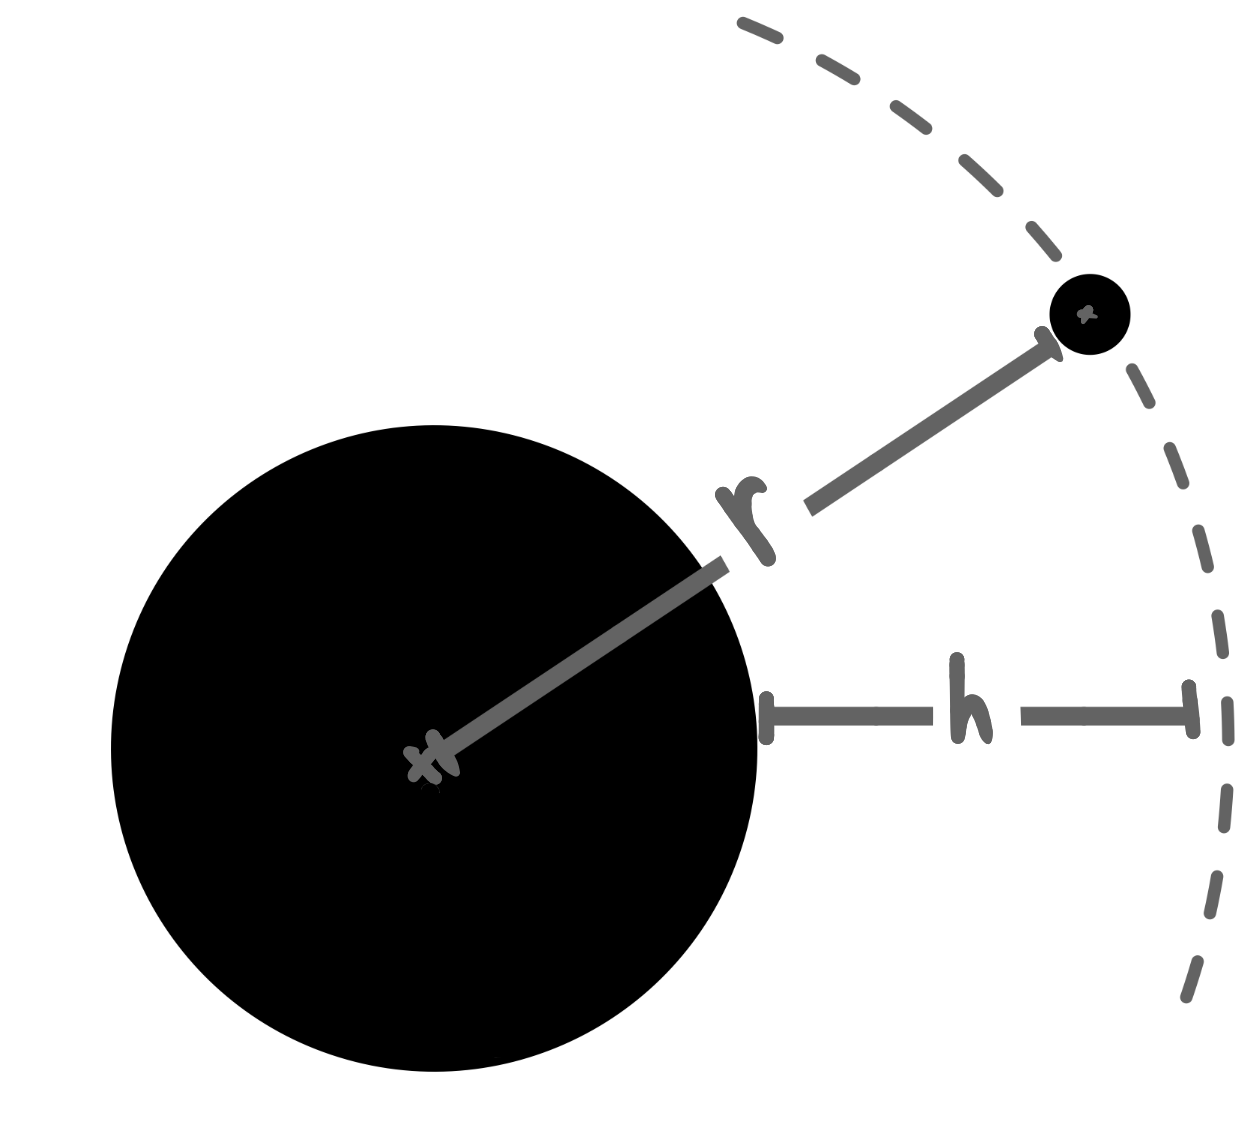
\includegraphics[width=0.3\linewidth]{imagensgravitacao/newtonleigravitacao.png}
\captionof{figure}{A distância $r$ entre corpos extensos é tomada em relação aos seus centros.}
\label{fig_gravitacao_leigravitacaouniversal}
} 
\vspace{0.3cm}

    \item [(ii)] Dobrar a distância e esperar que a força caia pela metade.
    
A força gravitacional segue uma lei do inverso do quadrado. Se a distância dobra, a força não cai pela metade — ela cai para \textbf{um quarto}. Esse erro é consequência de não internalizar o expoente~2 no
denominador. Ao triplicar a distância a força irá cair pelo fator $3^2=9$, ficando nove vezes menor. Ao quadriplicar a distância a força fica $4^2=16$ vezes menor, e por aí vai. A força, portanto, não é inversamente proporcional à distância, mas sim inversamente proporcional ao quadrado da distância.
    
\end{enumerate}



\secgfe{Observações}

Uma primeira observação é quanto à constante de gravitação $G$ ter um valor muito pequeno: $G= 6.67 \cdot 10^{-11} \text{N}\cdot\text{m}^2 \cdot \text{kg}^{-2}.$ Isso faz com que a força de atração gravitacional seja uma \textit{força fraca}, isto é, para que ela seja relevante é preciso que os valores das massas sejam muito grandes, do contrário, ela é praticamente irrelevante.

Considere, por exemplo, a força de atração entre dois indivíduos de $75$ quilogramas de massa, separados por apenas 1 metro. A força de atração gravitacional entre eles seria

$$ F= \dfrac{GMm}{r^2} = \dfrac{6.67 \cdot 10^{-11} \text{N}\cdot\text{m}^2 \cdot \text{kg}^{-2} \cdot 75 \text{ kg}  \cdot 75 \text{ kg}}{(1 \text{ m)}^2} \implies F = 3.75 \cdot 10^{-7} \text{ N},$$

\noindent ou seja, uma força de $0.000000375$ N. Para efeitos comparativos, o peso de um grão de areia é uma força maior do que isso. E é por isso que você nunca se sentiu atraído gravitacionalmente por ninguém -- exceto pela Terra.

Portanto, a força gravitacional, apesar de se manifestar em quaisquer corpos massivos, só será de fato relevante para corpos que tenham realmente muita massa, como uma estrela ou um planeta, haja vista que é preciso enormes valores de $M$ e $m$, posto o pequeno valor da constante de gravitação universal $G.$

Uma segunda observação interessante é sobre a relação entre a Terceira Lei de Kepler e a Lei da Gravitação Universal. Conforme discutido, a Lei da Gravitação de Newton foi modelada como sendo a força de atração entre corpos massivos que gerasse movimentos compatíveis com aqueles observados por Kepler, e registrado em suas leis.  Para ilustrar essa relação podemos, por exemplo, demonstrar a Terceira Lei de Kepler usando a Lei da Gravitação Universal, que pode ser feito como se segue.

Considere um satélite de massa $m$ em uma órbita circular, em torno de um planeta de massa $M.$ A força gravitacional atua como resultante centrípeta, o que se escreve como

$$ F_\text{G} = F_\text{CPT} \implies \dfrac{GMm}{r^2} = \dfrac{mv^2}{r} \implies v^2 = \dfrac{GM}{r}.$$

Sendo a órbita circular, $r$ é constante, de modo que a velocidade $v$ também o é. O movimento, portanto, trata-se de um MCU, de modo que é possível escrever

$$ v = \dfrac{d}{t} = \dfrac{2 \pi r}{T},$$

\noindent o que, na relação anterior, produz

$$ \left(  \dfrac{2 \pi r}{T}  \right)^2 = \dfrac{GM}{r} \implies \boxed{\dfrac{T^2}{r^3} = \dfrac{4 \pi^2}{GM}.}$$

Ou seja, a razão entre o quadrado do período $T$ e o cubo do raio da órbita $r$ é uma constante que depende exclusivamente da massa $M$ em torno do qual o satélite está orbitando. Sendo assim, para quaisquer satélites que orbitem o mesmo planeta tal valor será sempre o mesmo, como diz a Terceira Lei de Kepler.

\vspace{0.3cm}


\begin{exemplo}[Nível I]\label{exemplo_gravitacao_leigravitacaouniversalex01}

Um objeto de 5 kg está na superfície de um planeta esférico, chamado Terra, cuja massa é $M = 6.0 \cdot 10^{24}$ kg e cujo raio é $R = 6.4 \cdot 10^{6}$ m. Calcule a força gravitacional que o planeta exerce sobre o objeto.
Dado: $G = 6.67 \cdot 10^{-11}$ N{\cdot}m²/kg².

\resolucao

\[
  F = G\frac{Mm}{R^2}
    = 6.67 \cdot 10^{-11} \cdot
      \frac{6.0 \cdot 10^{24} \cdot 5.0}{(6.4 \cdot 10^{6})^2}
\]

\[
  F = 6.67 \cdot 10^{-11} \cdot
      \frac{3.0 \cdot 10^{25}}{4.096 \cdot 10^{13}}
    \approx {48.9\ \text{N}}
\]

Note que esse é exatamente o peso do objeto na Terra ($P = mg = 5 \cdot 9.8 = 49$ N), o que nos mostra que o valor da aceleração da gravidade $g$ seria dado pela expressão $g = GM/R^2$. Exploraremos este fato na definição de campo gravitacional, no estudo da Equação \eqref{eq_newton_campogravitacional}.

\end{exemplo}



\vspace{0.3cm}



\begin{exemplo}[Nível II]\label{exemplo_gravitacao_leigravitacaouniversalex02}


A figura representa dois planetas, de massas $m_1$ e $m_2$, cujos centros estão separados por uma distância $D$, muito maior que os raios dos planetas.

\begin{center}
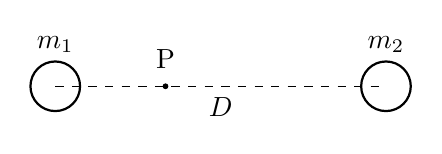
\begin{tikzpicture}[scale=0.7]

    % Planeta esquerdo
    \draw[thick] (0,0) circle (0.45);
    % \draw[thick] (-0.15,0) -- (0.15,0);
    % \draw[thick] (0,-0.12) -- (0,0.12);
    \node at (0,0.75) {$m_1$};

    % Planeta direito
    \draw[thick] (6,0) circle (0.45);
    % \draw[thick] (5.85,0) -- (6.15,0);
    % \draw[thick] (6,-0.12) -- (6,0.12);
    \node at (6,0.75) {$m_2$};

    % Linha tracejada entre centros
    \draw[dashed] (0,0) -- (6,0);

    % Ponto P
    \fill (2,0) circle (1.5pt);
    \node at (2,0.5) {P};

    % Distância D
    \node at (3,-0.38) {$D$};

    % Referência do ponto a D/3 de m1 (opcional visual)
    % Se quiser marcar explicitamente:
    % \draw[<->] (0,-0.8) -- (2,-0.8);
    % \node at (1,-1.05) {$D/3$};

   

\end{tikzpicture}
\end{center}

Sabendo que é nula a força gravitacional sobre uma terceira massa colocada no ponto $P$, a uma distância $\sfrac{D}{3}$ de $m_1$, encontre a razão $m_1/m_2$ entre as massas dos planetas.



\resolucao

Seja $m$ o valor da massa que será colocada no ponto $P.$ A força de atração $F_1,$ feita sobre o planeta de massa $m_1$ sob tal corpo, deve ser anulada pela força $F_2,$ feita sobre o planeta de massa $m_2$ sob tal corpo. Usando a Equação \eqref{eq_gravitacao_leigravitacaouniversal}, teremos:

$$ F_1 = F_2 \implies \dfrac{Gm_1 \cancel m}{\left( \dfrac{D}{3} \right)^2} = \dfrac{Gm_2 \cancel m}{\left( \dfrac{2D}{3} \right)^2} \implies \dfrac{9m_1}{1} =  \dfrac{9m_2}{4} \implies \boxed{\dfrac{m_1}{m_2} = \dfrac{1}{4}.} $$

Interpretando o resultado: como a massa $m_1$ está duas vezes mais próxima de $P$ do que $m_2,$ tendo metade da distância, a força seria $2^2 = 4$ vezes maior. Contudo, para gerar a mesma força, basta ter quatro vezes menos massa para que esses efeitos se anulem, e é por isso que a massa $m_1$ é quatro vezes menor do que $m_2.$



\end{exemplo}



\vspace{0.3cm}



\begin{exemplo}[Nível III (ITA - 2018)]\label{exemplo_gravitacao_leigravitacaouniversalex03}

Quatro corpos pontuais, cada qual de massa $m$, atraem-se mutuamente devido à interação gravitacional. Tais corpos encontram-se nos vértices de um quadrado de lado $L$ girando em torno de seu centro com velocidade angular constante. Sendo $G$ a constante de gravitação universal, o período dessa rotação é dado por:

\begin{itemize}
    \item[(a)] $2\pi \sqrt{\frac{L^3}{Gm} \left(\frac{4 - \sqrt{2}}{2}\right)}$
    
    \item[(b)] $\frac{4\pi}{3} \sqrt{\frac{\sqrt{2} \, L^3}{3Gm}}$
    
    \item[(c)] $\sqrt{\frac{L^3}{Gm} \left(\frac{4 + \sqrt{2}}{7}\right)}$
    
    \item[(d)] $2\pi \sqrt{\frac{L^3}{Gm} \left(\frac{4 - \sqrt{2}}{7}\right)}$
    
    \item[(e)] $\sqrt{\frac{L^3}{Gm} \left(\frac{4 + \sqrt{2}}{2}\right)}$
\end{itemize}


\resolucao

Avaliando a força em uma única massa, teremos:

$$ F_1=F_2 = F= \dfrac{Gm^2}{L^2} \quad \text{ e } \quad F_3 = \dfrac{Gm^2}{(L\sqrt 2)^2} = \dfrac{Gm^2}{2L^2}.$$

\vspace{0.3cm}
{
\centering
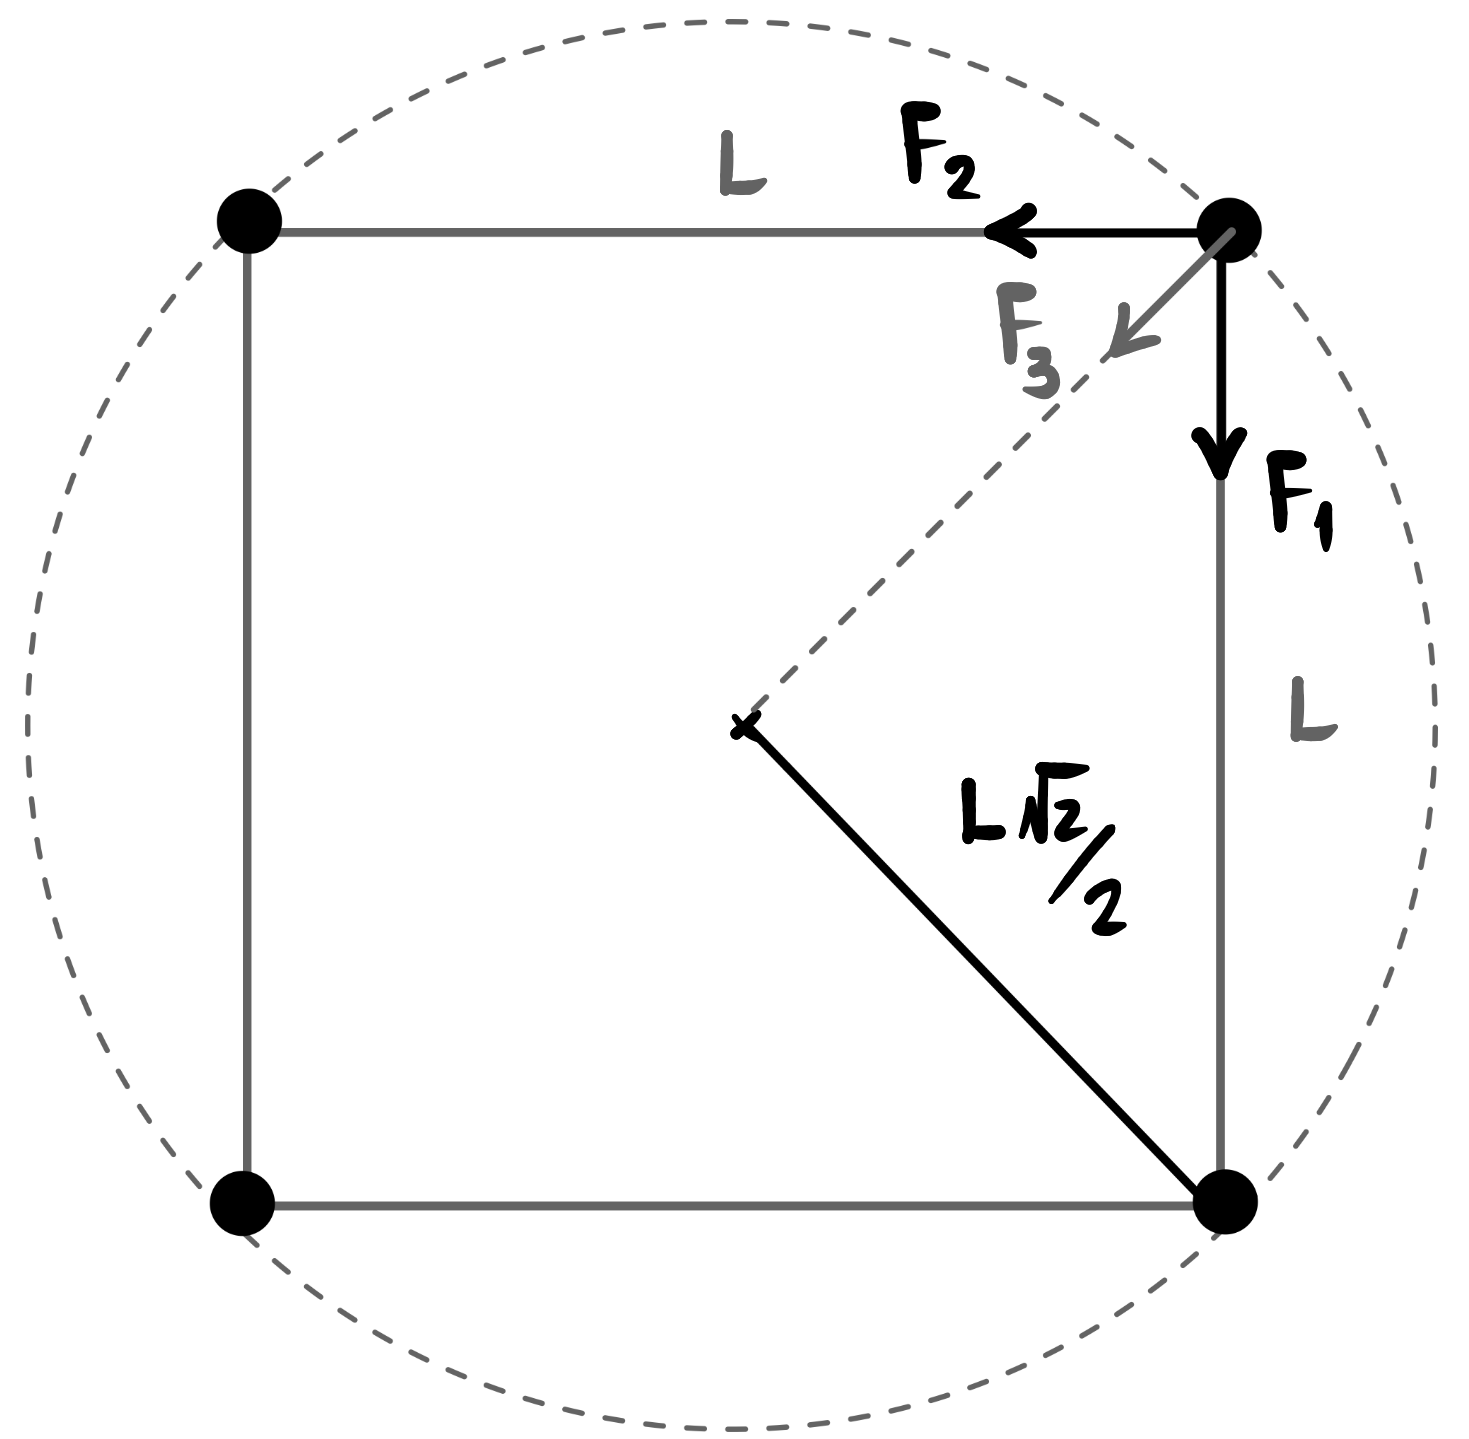
\includegraphics[width=0.35\linewidth]{imagensgravitacao/gravitacaoitaexemplonivel3.png}
\captionof{figure}{}
\label{fig_gravitacao_leigravitacaouniversal2}
} 
\vspace{0.3cm}


Fazendo a força resultante, teremos a resultante entre $F_1$ e $F_2$ sendo dadas pelo Teorema de Pitágoras, valendo $F\sqrt 2,$ e apontando exatamente na direção da diagonal do quadrado, que é a direção de $F_3.$ Logo, a força resultante é

$$ F_\text{R} = F_3 + F\sqrt 2 = \dfrac{Gm^2}{2L^2} + \dfrac{\sqrt 2Gm^2}{L^2} = \dfrac{Gm^2}{2L^2} (1 + 2\sqrt 2).$$

Tal força atua como resultante centrípeta, de modo que 

$$ F_{\text{R}_{CPT}} = m\omega^2r = m\omega^2 L \dfrac{\sqrt 2}{2} = \dfrac{Gm^2}{2L^2} (1 + 2\sqrt 2),$$

\noindent de onde vem que $\omega = \sqrt{\dfrac{Gm}{\sqrt2L^3} (1 + 2\sqrt 2)}, $ e, usando $\omega = \sfrac{2 \pi}{T}$, teremos

$$ \boxed{T = 2 \pi \sqrt{\dfrac{L^3}{Gm} \left(  \dfrac{4- \sqrt 2}{7}\right) \implies \text{ letra D} .}}$$


\end{exemplo}












\begin{secnivel}[Velocidade Orbital]{II}{Velocidade Orbital de um Satélite}
 

  \eqLdois{dem}{eq_gravitacao_velocidadeorbital}{v_o = \sqrt{\dfrac{GM}{(R+h)}}}
  
\end{secnivel}




\secgfe{De onde vem}

Como discutido no desenvolvimento da Equação \eqref{eq_gravitacao_leigravitacaouniversal}, o movimento orbital e a queda livre são diferentes manifestações de um mesmo fenômeno. A Figura \ref{fig_gravitacao_experimentobaladecanhao} nos permite enxergar isso com clareza, em um experimento mental realizado por Newton, conhecido como experimento da bala de canhão. Os desenhos de tal figura são tal e qual foram feitos por Newton, e o argumento construído por ele se dá como se segue.

Imagine que estamos no topo de uma montanha, com um canhão, e iremos fazer alguns disparos. Como é de se esperar, devido à atração gravitacional da Terra, a bala de canhão cairá enquanto avança horizontalmente, até eventualmente colidir com a superfície da Terra. Se aumentarmos sua velocidade de lançamento, como mostra a segunda e terceira imagem, a bala avançará mais enquanto cai, colidindo com a superfície da Terra em um ponto mais distante. 



\vspace{0.3cm}
{
\centering
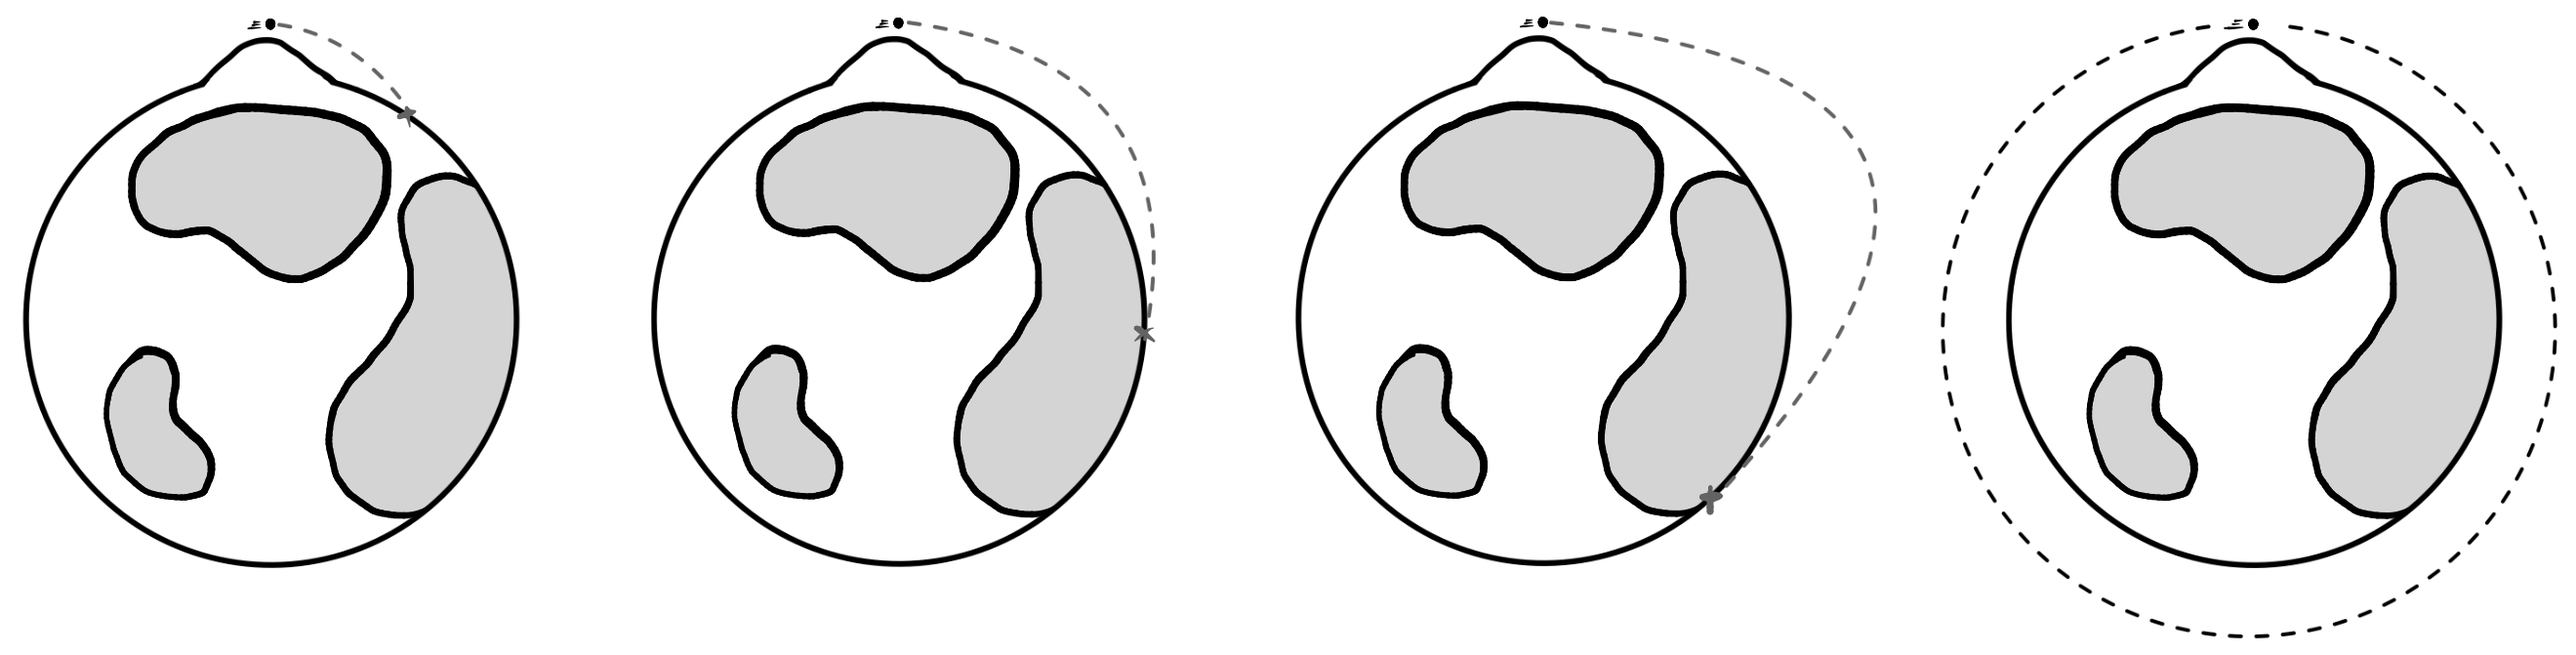
\includegraphics[width=1.0\linewidth]{imagensgravitacao/experimentobaladecanhao.png}
\captionof{figure}{O experimento da bala de canhão de Newton.}
\label{fig_gravitacao_experimentobaladecanhao}
} 
\vspace{0.3cm}

O argumento do Newton é que se ajustarmos e aumentarmos o suficiente essa velocidade a bala irá cair...porém conseguirá completar uma volta antes de colidir com a superfície da Terra. Nesse caso, ela entrou em órbita: a velocidade é aquela exata para que a bala caia, porém sem nunca colidir com a superfície terrestre. É o que aparece ilustrado na última imagem da Figura \ref{fig_gravitacao_experimentobaladecanhao}.


Sendo assim, é preciso que haja uma certa harmonia -- um equilíbrio exato -- entre a velocidade de lançamento do satélite e o campo gravitacional do planeta, a fim de que seja possível o movimento orbital. Para uma velocidade pequena demais o satélite irá cair e colidir com a superfície do planeta em algum ponto. Se a velocidade for alta demais será possível que o satélite escape do campo gravitacional do planeta e nunca mais volte -- isso será calculado pela Equação \eqref{eq_newton_velocidadeescape}. Buscamos a velocidade exata que o satélite deve ter para ficar entre essas duas situações: confinado pelo campo gravitacional do planeta, porém caindo sem nunca colidir contra sua superfície. Neste caso -- em uma queda livre eterna -- dizemos que o satélite entrou em órbita.

Para calcular o valor exato de tal velocidade, considere um satélite de massa $m$ orbitando um planeta de massa $M$ e raio $R.$ Assumindo que se trata de uma órbita circular de altitude $h$ (distância até a superfície da terra), o satélite estará descrevendo uma circunferência de raio $r=(R+h)$ em torno do centro do planeta esférico, como mostra a Figura \ref{fig_gravitacao_velocidadeorbitalimagem}.


\vspace{0.3cm}
{
\centering
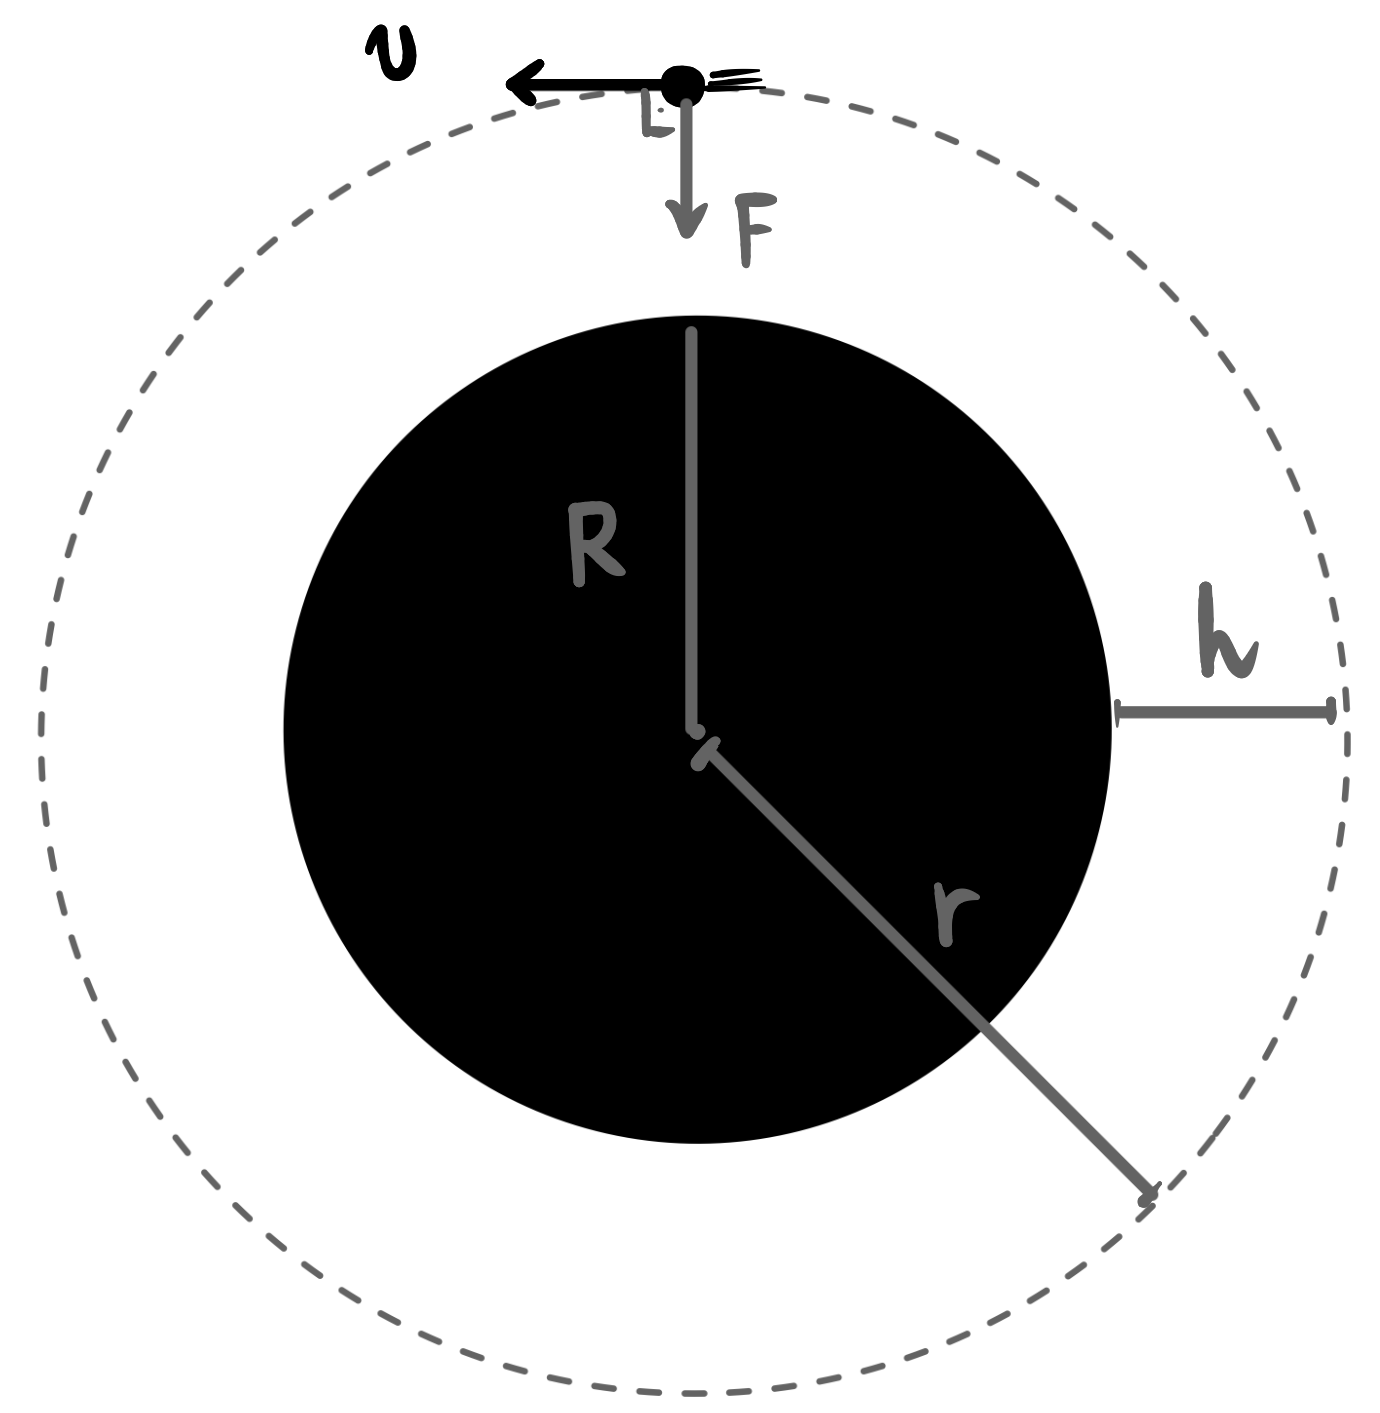
\includegraphics[width=0.3\linewidth]{imagensgravitacao/velocidadeorbitalimagem.png}
\captionof{figure}{Satélite na órbita de raio $r=R+h.$}
\label{fig_gravitacao_velocidadeorbitalimagem}
} 
\vspace{0.3cm}


A força de atração gravitacional -- perpendicular à velocidade do satélite e apontando para o centro da trajetória -- é a nossa força resultante centrípeta. Desse modo, usando as Equações \eqref{eq_gravitacao_leigravitacaouniversal} e \eqref{eq_newton_forcacentripeta}, temos

$$ F_G = F_{\text{R}_{CPT}} \implies \dfrac{GM \cancel m}{r^ 2} = \dfrac{\cancel mv_0^2}{ r}, $$

\noindent de onde já notamos que a velocidade $v_0$ que o satélite deve ter para se manter em tal órbita não depende de sua massa $m$: satélites de quaisquer massas precisarão exatamente da mesma velocidade $v_0$ para se manterem em tal órbita. Desenvolvendo, teremos

$$ \dfrac{GM }{r^ \cancel2} = \dfrac{v_0^2}{ \cancel r} \implies v_0 = \sqrt{\dfrac{GM}{r}} = \sqrt{\dfrac{GM}{R+h}},$$
 
\noindent como diz a Equação \eqref{eq_gravitacao_velocidadeorbital}.

Perceba que a Equação \eqref{eq_gravitacao_velocidadeorbital} é condizente com o esperado: quanto maior for o valor da massa $M$ do planeta, maior deverá ser o valor da velocidade do satélite para se manter naquela órbita. Isso ocorre porque um planeta mais massivo possui uma atração gravitacional mais intensa, de modo que a tendência do satélite cair (e colidir contra superfície do planeta) é maior, de tal sorte que será necessária uma velocidade maior a fim de que ele consiga escapar disso: continuar caindo, porém sem nunca colidir com a superfície do planeta -- isso é entrar em órbita.\footnote{Uma curiosidade: é exatamente por isso que astronautas não sentem o próprio peso. Muitos pensam que astronautas, em um satélite, estão em um ponto de gravidade zero, e por isso ficam flutuando. Mas isso está errado. O valor da gravidade na estação espacial internacional (ISS) é apenas 10\% inferior da gravidade na superfície da Terra. O que acontece é que a ISS, por estar orbitando a Terra, está em uma queda livre eterna, e, um corpo em queda livre, não sente o próprio peso. Se imagine caindo, no meio do espaço: você sentiria o próprio peso? Ou teria a sensação de estar flutuando...? Essa, para Einstein, foi a ideia mais linda que ele já teve.}




\secgfe{Onde é usada}

A Equação \eqref{eq_gravitacao_velocidadeorbital} é usada para computar a velocidade de satélites que executam órbitas circulares em torno de um certo astro devido à ação da força gravitacional exercida por tal astro.


\secgfe{Erros comuns}

O erro mais comum aqui seria o de confundir o raio do planeta $R$ com o raio da órbita do satélite $r$. Se o satélite orbitar tangenciando a superfície da terra, bem próximo dessa, ou seja, com $ h \approx 0,$ essas duas grandezas serão praticamente iguais:

$$ r = R + \cancelto{0}{h} \implies r \approx R.$$

Contudo, quanto maior for a distância $h$ do satélite em relação à superfície da terra, as duas grandezas começam a se diferenciar. Portanto, note que aquilo que entra no denominador da Equação \eqref{eq_gravitacao_velocidadeorbital} é o raio da órbita do satélite $r=R+h,$ e não o raio $R$ do planeta em torno do qual ele orbita.

\secgfe{Observações}


É importante que o estudante note que o processo de construção da Equação \eqref{eq_gravitacao_velocidadeorbital} é exatamente o mesmo para se construir as Equações \eqref{eq_newton_velocidadeloop} ou \eqref{eq_newton_velocidademinimaparacurva}: trata-se apenas de identificar a resultante das forças na direção do centro -- no caso, a força gravitacional -- e usar a Segunda Lei de Newton:

$$ F_{R_{\text{CPT}}} = m a_{\text{CPT}} = m \dfrac{v^2}{R}.$$

Ou seja, tudo o que se precisa saber é como computar a força gravitacional, a Segunda Lei de Newton e a Equação \eqref{cinvet_eq_aceleracaocentripeta}, que fornece a aceleração centrípeta. Sendo assim, é importante que o leitor compreenda a construção da Equação \eqref{eq_gravitacao_velocidadeorbital} e saiba fazê-la ao invés de escolher o cômodo, fácil e ineficaz caminho de apenas memorizá-la.



Por fim, para tirar a limpo com o leitor um último fato, retornemos à história de um corpo que cai sem nunca colidir contra a superfície da Terra -- que é o que designamos como movimento orbital. Perceba que isso só é possível em um planeta que não seja plano. Para compreender isso, considere que faremos um lançamento horizontal de um certo corpo a partir de uma certa altitude em relação à superfície do planeta -- como no experimento da bala de canhão de Newton. A Figura \ref{fig_gravitacao_terraplana} ilustra isso.



\vspace{0.3cm}
{
\centering
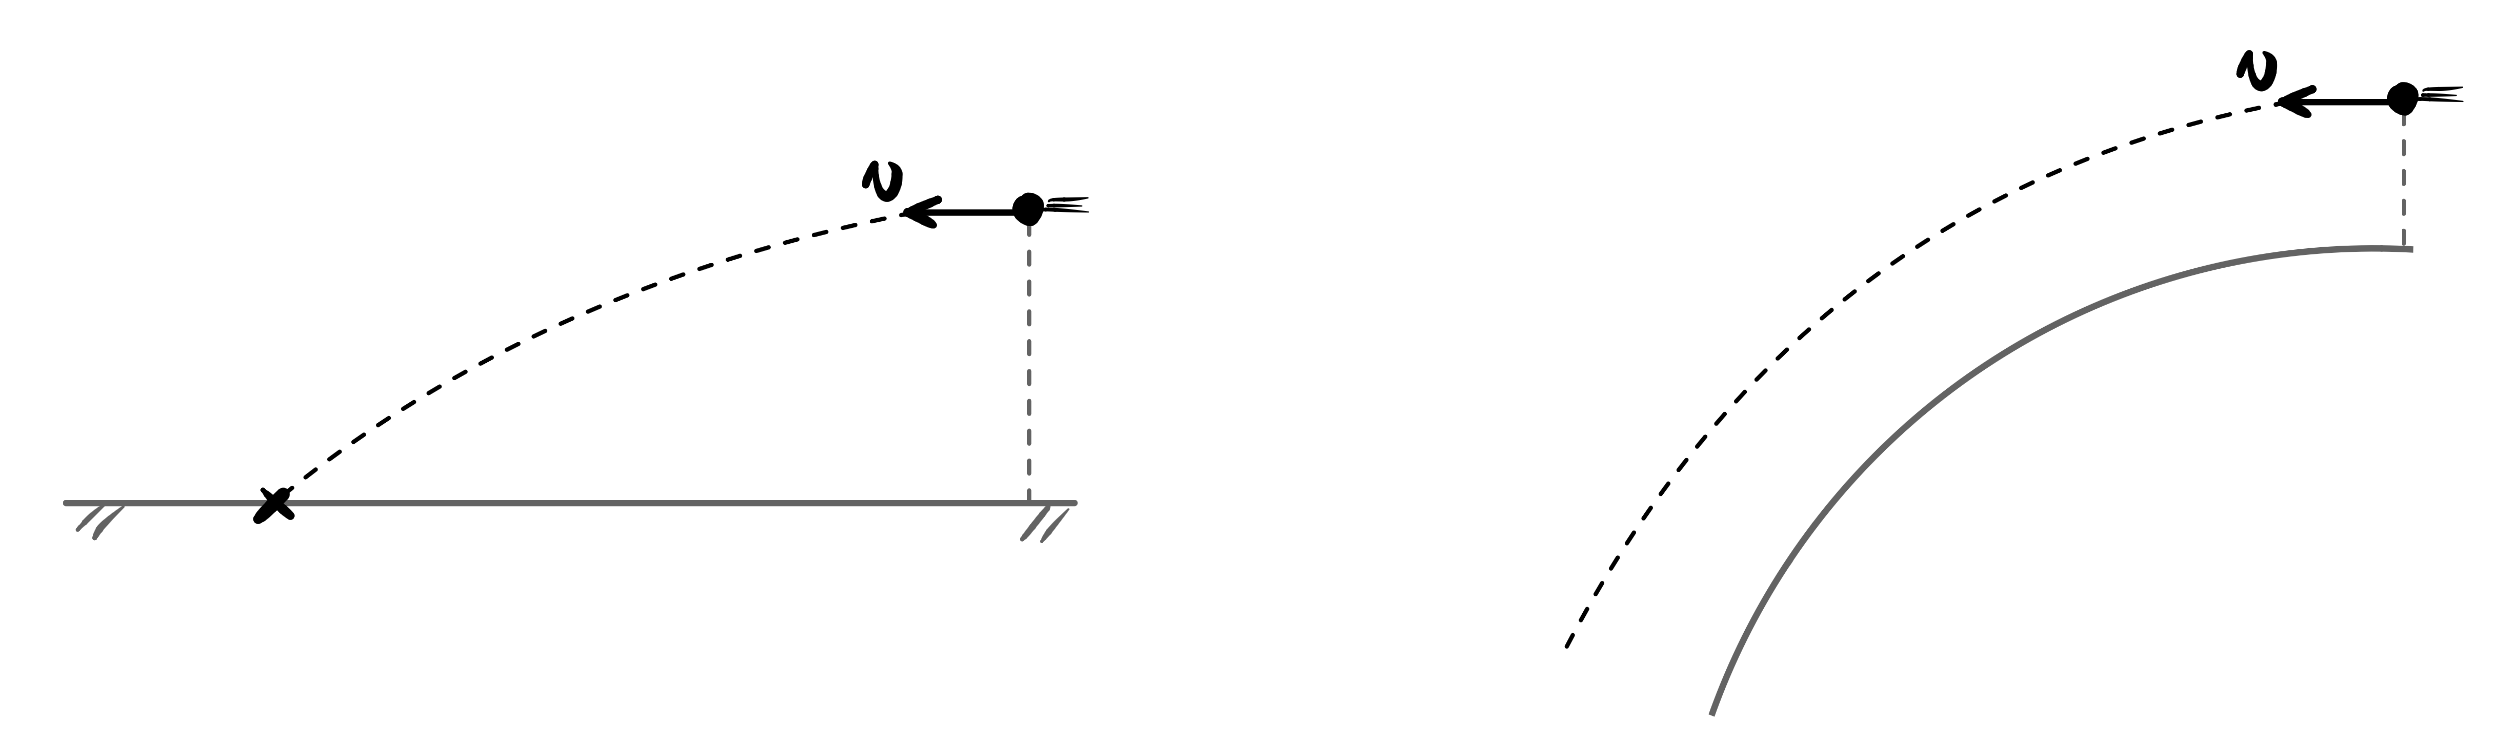
\includegraphics[width=0.8\linewidth]{imagensgravitacao/terraplana.png}
\captionof{figure}{O movimento de queda, composto com uma velocidade tangencial, para planetas de diferentes curvaturas.}
\label{fig_gravitacao_terraplana}
} 
\vspace{0.3cm}



Para uma Terra plana, como mostra a primeira imagem, o destino é inequívoco: o corpo que está caindo invariavelmente haverá de colidir com a superfície do planeta. Contudo, para uma Terra que não seja plana, é possível que, ao longo da queda, caso ela se dê acompanhando a curvatura da Terra, o corpo consiga cair eternamente, sem nunca colidir com a superfície do planeta. Portanto, o movimento orbital, neste sentido, só é possível em um planeta que não seja plano -- caso o leitor estivesse em dúvida sobre seu formato, eis um bom argumento para convencê-lo.



\vspace{0.3cm}

\begin{exemplo}[Nível I]\label{exemplo_gravitacao_velocidadeorbitalex01}

Um satélite geoestacionário é aquele que está parado em relação à Terra. Encontre qual é a altitude em que este satélite deve estar para estar em tal órbita.

Considere que a massa da Terra é $M=6 \cdot 10^{24}$ kg e seu raio é $R=6.400$ km.

\resolucao

Se o satélite fica parado em relação à Terra, isso significa que ele gira exatamente junto da Terra, ou seja, possui a mesma velocidade angular $\omega$ da Terra:

$$ \omega = \dfrac{2 \pi}{T} = \dfrac{2 \pi}{24 \cdot 3600 \text{ seg}} \approx \dfrac{1}{14.400} \text{s}^{-1}.$$

Assim, usando as Equações \eqref{eq_gravitacao_velocidadeorbital} e \eqref{cinvet_eq_velangularelinear}, segue que

$$ \sqrt{\dfrac{GM}{r}} = \omega r \implies r^3 = \dfrac{GM}{\omega^2}.$$

Assim, substituindo os valores, teremos

$$ r^3 = \dfrac{6 \cdot 10^{24}  \cdot 6.6 \cdot 10^{-11}}{\left( \dfrac{1}{14.400} \right)^2} \approx 82 \cdot 10^{21}.$$

Extraindo a raiz cúbica, teremos $r \approx 4.34 \cdot 10^{7}$m = $43.400$ km. Logo, a altitude $h$ do satélite é tal que 
$$r=R+h \implies h = r-R = 43.400 - 6400 \approx \boxed{37.000 \text{ km}.} $$


\end{exemplo}

\vspace{0.3cm}

\begin{exemplo}[Nível II]\label{exemplo_gravitacao_velocidadeorbitalex02}

Dois satélites, $A$ e $B,$ estão orbitando um mesmo planeta. Se a velocidade orbital de $A$ é o dobro da de $B,$ e se a altitude de $B$ é igual a $4R$, qual é a distância de $A$ até a superfície da Terra?

\resolucao

Usando a Equação \eqref{eq_gravitacao_velocidadeorbital}, segue que

$$ \dfrac{v_A}{v_B} = \dfrac{\sqrt{\dfrac{GM}{(R+h_A)}}}{\sqrt{\dfrac{GM}{(R+h_B)}}} = 2.$$

Simplificando alguns termos e quadrando dos dois lados, teremos

$$ \dfrac{R+h_B}{R+h_A} = 4 \implies  R + h_B = 4R + 4h_A \implies h_B - 4h_A = 3R. $$

Como $h_B = 4R$, segue da relação acima que $\boxed{h_A = R/4.}$


\end{exemplo}

\vspace{0.3cm}

\begin{exemplo}[Nível III]\label{exemplo_gravitacao_velocidadeorbitalex03}


Dois satélites descrevem órbitas circulares ao redor da Terra. O satélite A está a uma altura $h$ da superfície, enquanto o satélite B está a uma altura $3h$.

Sabendo que $h \ll R$, onde $R$ é o raio da Terra, a razão entre as velocidades orbitais de $A$ e $B$ pode ser melhor aproximada por:

\begin{enumerate}
    \item [a)] $1 + \dfrac{h}{R}$
    \item [b)] $1 + \dfrac{h}{2R}$
    \item [c)] $1 + \dfrac{3h}{2R}$
    \item [d)] $1 + \dfrac{2h}{3R}$
    \item [e)] $1 - \dfrac{3h}{2R}$
\end{enumerate}


\resolucao

O formato das expressões nas alternativas já nos convida a lembrar da aproximação binomial, que diz que

$$ (1+x)^n \approx 1 +nx \quad \text{ se } \quad x<<1.$$

Neste caso, temos a expressão

$$ \sqrt{\dfrac{GM}{R+h}},$$

\noindent com $h<<R.$ Vamos tentar escrever a expressão em termos de $\sfrac{h}{R},$ uma vez que 

$$h<<R \implies \sfrac{h}{R} << 1,$$ 

\noindent que é a condição da aproximação binomial. Façamos isso fatorando o termo $R$ no denominador:

$$ \sqrt{\dfrac{GM}{R+h}} = \sqrt{\dfrac{GM}{R \left(1+ \dfrac{h}{R} \right)}} = \sqrt{\dfrac{GM}{R}} \left( 1+ \dfrac{h}{R}\right)^{-1/2}. $$

Note que temos, no termo final entre parênteses, justamente o formato exigido pela aproximação binomial: $(1+x)^n,$ em que $x=\sfrac{h}{R}<<1.$ Logo, teremos

$$ \left( 1+ \dfrac{h}{R}\right)^{-1/2} \approx 1 -\dfrac{h}{2R}.$$ 

Assim, a velocidade orbital, usando tal aproximação, pode ser expressa como

$$ v_o =  \sqrt{\dfrac{GM}{R}} \left( 1 -\dfrac{h}{2R} \right). $$

Desse modo, fazendo a razão entre $v_A$ e $v_B$ teremos

$$ \dfrac{v_A}{v_B} = \dfrac{ \sqrt{\dfrac{GM}{R}} \left( 1 -\dfrac{h}{2R} \right)}{ \sqrt{\dfrac{GM}{R}} \left( 1 -\dfrac{3h}{2R} \right)} = \dfrac{\left( 1 -\dfrac{h}{2R} \right)}{\left( 1 -\dfrac{3h}{2R} \right)} = \left( 1 -\dfrac{h}{2R} \right) \cdot \left( 1 -\dfrac{3h}{2R} \right)^{-1}.$$

Perceba que podemos usar novamente a aproximação binomial para o segundo termo, fazendo que

$$ \left( 1 -\dfrac{3h}{2R} \right)^{-1} \approx 1 + \dfrac{3h}{2R},$$

\noindent de modo que somos levados a

$$ \dfrac{v_A}{v_B} = \left( 1 -\dfrac{h}{2R} \right) \cdot \left( 1 +\dfrac{3h}{2R} \right) = 1 + \dfrac{3h}{2R}- \dfrac{h}{2R}  - \dfrac{3}{4} \left( \dfrac{h}{R} \right)^2 = 1 + \dfrac{h}{R} - \dfrac{3}{4} \left( \dfrac{h}{R} \right)^2,$$

\noindent e, como $\sfrac{h}{R} << 1,$ temos que o termo quadrático $(\sfrac{h}{R})^2$ será desprezível em comparação com termos da ordem de $\sfrac{h}{R}.$ Desprezando o último termo na equação acima, teremos

$$ \boxed{\dfrac{v_A}{v_B}  \approx 1 + \dfrac{h}{R} \implies \text{letra A.}} $$

\end{exemplo}






\begin{secnivel}[Campo Gravitacional]{I}{Campo Gravitacional}
 

 \eqLdois{def}{eq_newton_campogravitacional}{g = \dfrac{GM}{r^2}}
  
\end{secnivel}





\secgfe{De onde vem}

Considere um certo planeta de massa $M$. Em um ponto exterior a tal planeta, a uma distância $r$ do seu centro, vamos colocar corpos de diferentes massas e avaliar qual é a força gravitacional que eles sentem. A Figura \ref{fig_gravitacao_campogravitacional1} ilustra tal situação.


\vspace{0.3cm}
{
\centering
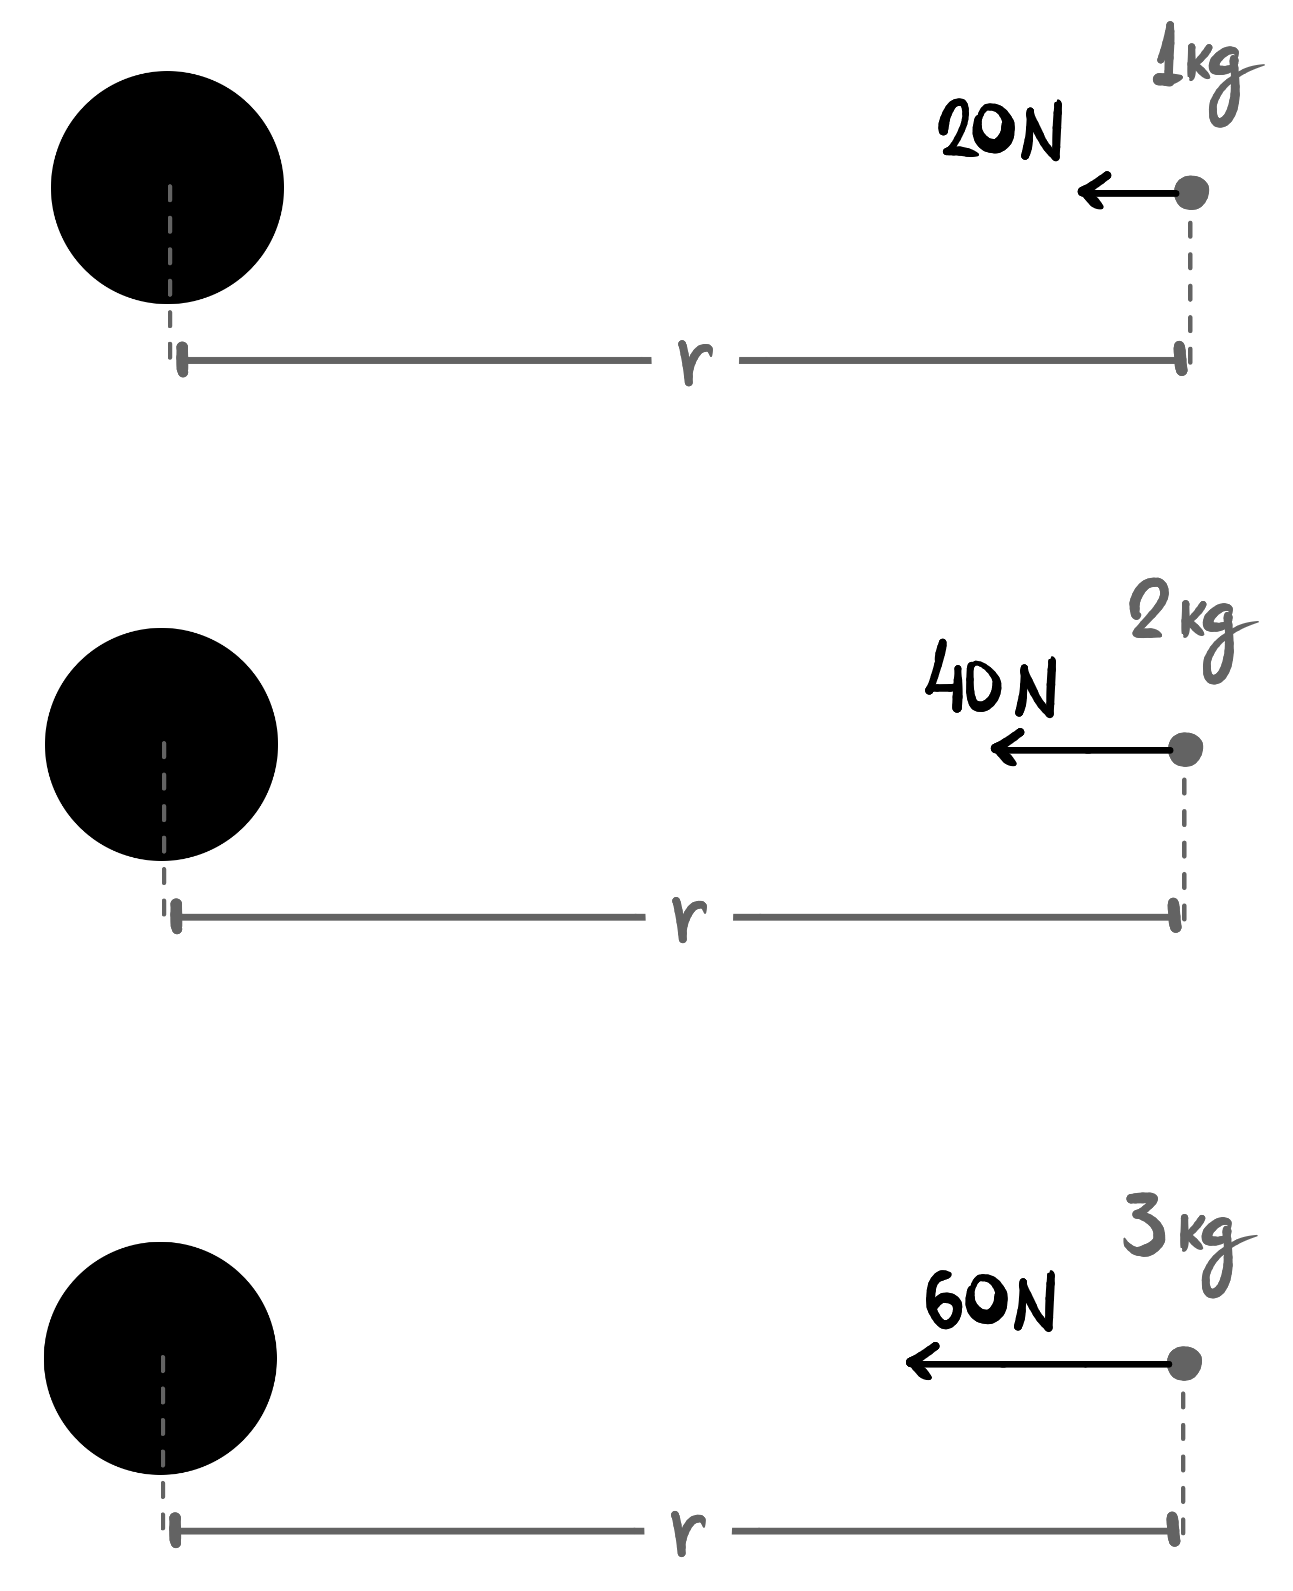
\includegraphics[width=0.4\linewidth]{imagensgravitacao/campogravitacional1.png}
\captionof{figure}{A força gravitacional sentida por uma certa massa $m$ é diretamente proporcional ao valor da sua massa.}
\label{fig_gravitacao_campogravitacional1}
} 
\vspace{0.3cm}

Como a própria Equação \eqref{eq_gravitacao_leigravitacaouniversal} evidencia, a força gravitacional sentida pelo corpo de massa $m$ é um valor diretamente proporcional à sua massa. Assim, ao fazer o cálculo usando tal expressão, para uma massa de $1$ kg, digamos que encontramos que o valor da força é de $20$N. É imediato que, para uma partícula que possua o dobro de massa, no caso, $2$ kg, a força gravitacional sentida por ela devido à massa $M$ será duas vezes maior, isto é, de $40$ N.

Caso a partícula tenha massa $m=3$ kg, a força gravitacional seria três vezes maior, valendo $60$N, como mostra a imagem. Perceba, portanto, que o valor da força gravitacional sentida por uma partícula em um certo ponto $P$, distante $r$ da partícula de massa $M$, depende de quem é a partícula colocada ali. Mais especificamente, depende do valor da sua massa $m.$


O conceito de campo gravitacional é criado justamente para representar uma propriedade do espaço que independe do valor de massa ali colocado. É fácil ver que a razão entre a força gravitacional sentida pela partícula de massa $m$ e a sua massa é uma constante, ou seja:

$$ \dfrac{20 \text{ N}}{1 \text{ kg}} =  \dfrac{40 \text{ N}}{2 \text{ kg}} = \dfrac{60 \text{ N}}{3 \text{ kg}}.$$

Ou seja, o valor de $20\text{N}/\text{kg}$ é um número fixo, que independe do valor da massa colocada ali. Qualquer que seja a massa $m$ colocada em tal ponto, ela sentirá uma força de $20$ N para cada quilograma de massa que tiver. Tal valor, portanto, é uma propriedade mais geral daquele ponto do espaço. Chamamos tal valor de campo gravitacional $g$ do planeta $M$ no ponto $P.$ Note, como mostra a Figura \ref{fig_gravitacao_campogravitacional2}, que o campo gravitacional $g$ criado pela massa $M$ no ponto $P$ é uma propriedade daquele ponto do espaço e independe de ter ou não alguma partícula ali. Ele representa a força por unidade de massa que qualquer partícula massiva colocada ali irá sentir.



\vspace{0.3cm}
{
\centering
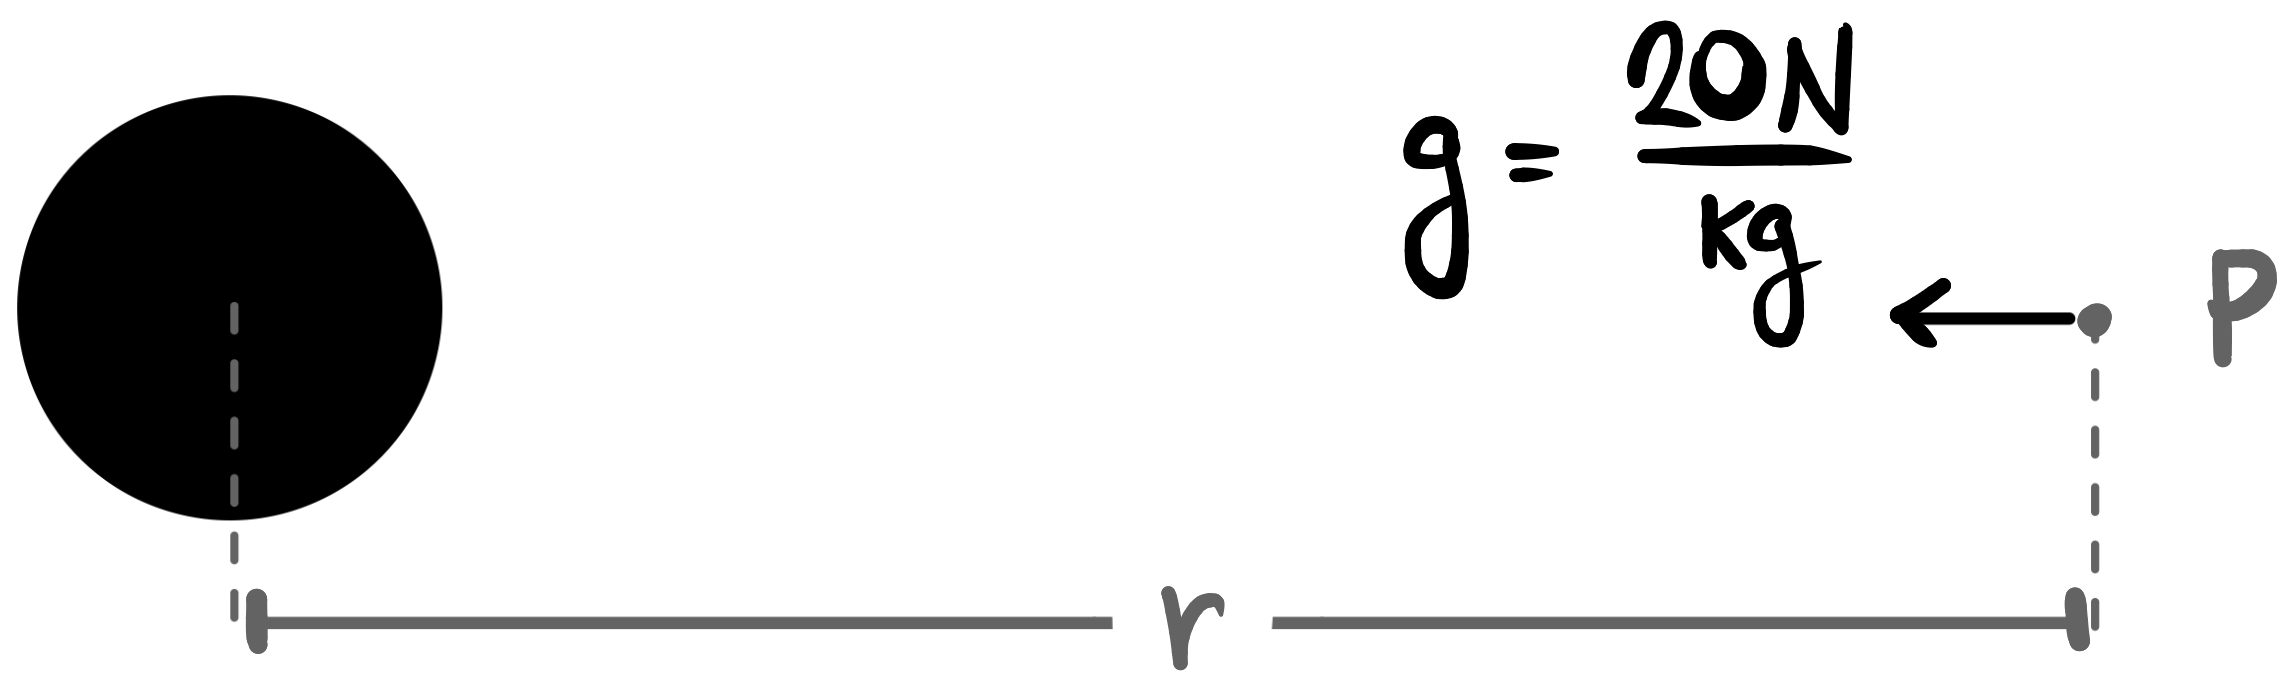
\includegraphics[width=0.4\linewidth]{imagensgravitacao/campogravitacional2.png}
\captionof{figure}{O campo gravitacional $g$ criado pela massa $M$ no ponto $P$ é um valor que depende apenas daquele ponto, e não da massa que será inserida ali.}
\label{fig_gravitacao_campogravitacional2}
} 
\vspace{0.3cm}


É exatamente por isso que Galileu tinha razão ao afirmar que todos os corpos caem com a mesma aceleração: porque $g$ não depende de $m$. A Segunda Lei de Newton diz que $F = ma$, logo $a = F/m = g$. A aceleração da queda livre é o próprio campo gravitacional local -- que é independente da massa do corpo.


O valor do campo gravitacional $g$, como vimos, é obtido pela razão entre a força gravitacional sentida por uma partícula de massa $m$ naquele ponto -- o que é dado pela Equação \eqref{eq_gravitacao_leigravitacaouniversal} -- e a sua própria massa $m$, isto é:

$$ g = \dfrac{F}{m} = \dfrac{\dfrac{GM\cancel m}{r^2}}{\cancel m} = \dfrac{GM}{r^2},$$

\noindent como expressa a Equação \eqref{eq_newton_campogravitacional}\footnote{Tal equação, portanto, fornece o valor do campo gravitacional $g$ de um planeta esférico, de massa $M$, em pontos que estão a uma distância $r$ do seu centro, desde que $r>R,$ em que $R$ é o raio do planeta.}.


Perceba que o valor do campo gravitacional $g$ em um certo ponto depende apenas da massa $M$ que cria aquele campo e da distância $r$ do ponto até a massa $M$ em questão. Dito isso, para uma mesma massa $M$, todos os pontos que estiverem a uma mesma distância $r$ dela terão o mesmo valor do campo gravitacional. Ou seja, todos os pontos que estiverem na superfície de uma esfera -- que é a superfície que contém todos os pontos que estão a uma distância $r$ de um certo dado ponto, o centro da esfera -- possuirão o mesmo campo gravitacional.

Além disso, esferas distintas terão campos distintos, que dependerão da sua distância $r$ até o centro do planeta que cria o campo gravitacional: quanto mais próximos do planeta, maior é o valor do campo gravitacional $g$, como expressa a Equação \eqref{eq_newton_campogravitacional}. Tal situação está ilustrada na Figura \ref{fig_gravitacao_campogravitacional3}.



\vspace{0.3cm}
{
\centering
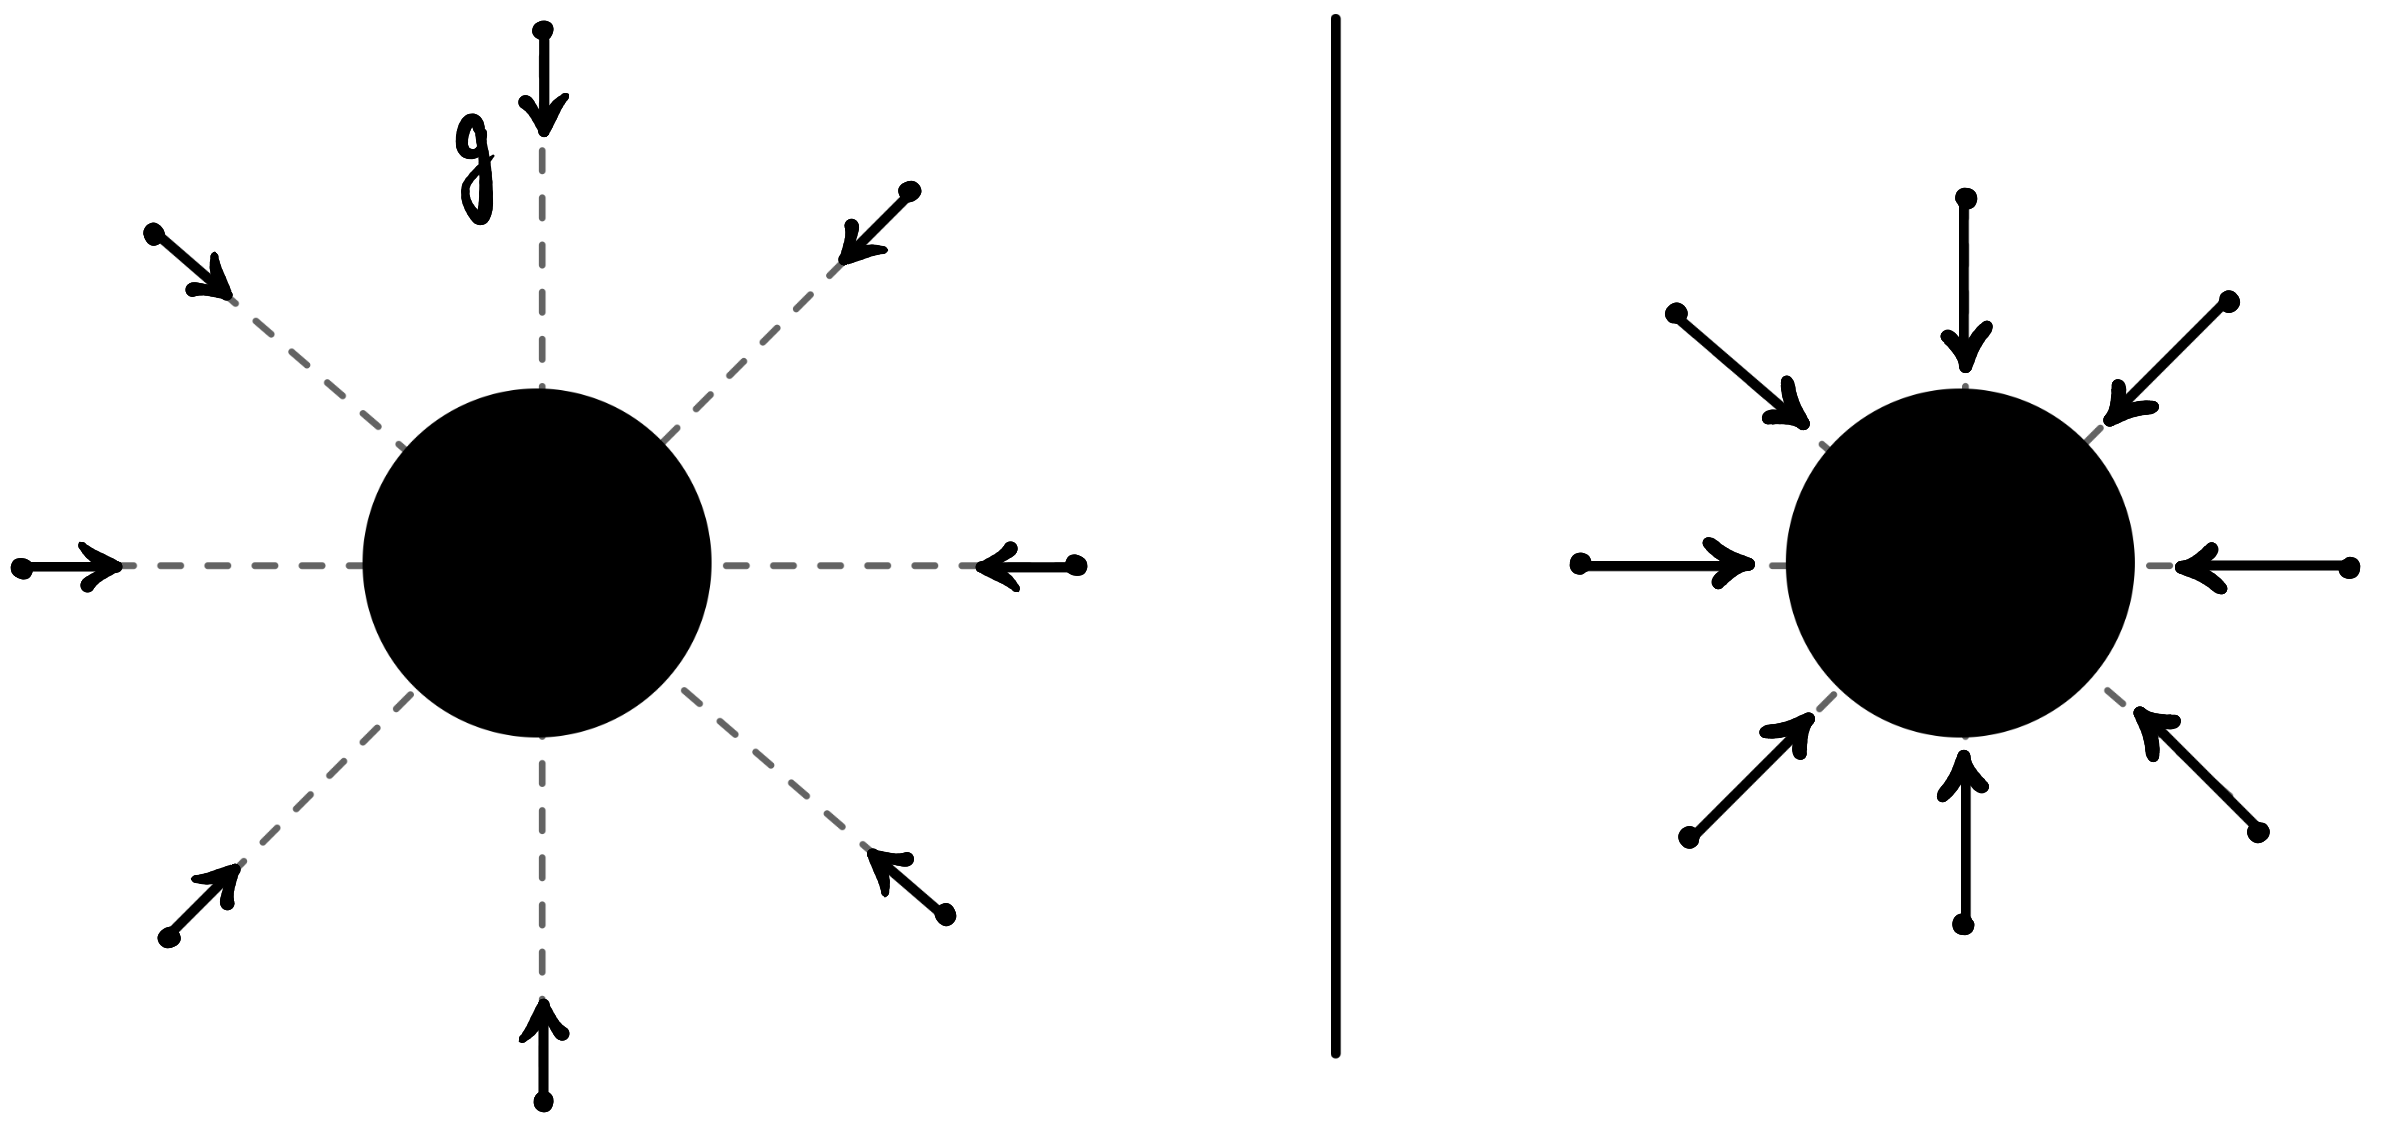
\includegraphics[width=0.6\linewidth]{imagensgravitacao/campogravitacional3.png}
\captionof{figure}{O campo gravitacional $g$ é inversamente proporcional ao quadrado da distância $r$.}
\label{fig_gravitacao_campogravitacional3}
} 
\vspace{0.3cm}

Uma propriedade geométrica do campo gravitacional pode ser observada na Figura \ref{fig_gravitacao_campogravitacional3}: quanto maior for a \emph{densidade de linhas de campo}, isto é, quanto mais próximas as linhas de campo estiverem (imagem da direita), mais intenso é o campo gravitacional. Quanto mais afastadas elas estiverem (imagem da esquerda), menos intenso é o campo gravitacional naquela região.




\secgfe{Onde é usada}

A Equação \eqref{eq_newton_campogravitacional} é usada para calcular o campo gravitacional de um planeta esférico de massa $M$ em um ponto que dista $r$ do centro de tal planeta (desde que tal ponto seja externo ao planeta). Em particular, se usamos $r=R$, teremos o campo gravitacional na superfície do planeta. Para a Terra, isso significa usar os valores da sua massa e do seu raio, que fornecem

$$ g = \dfrac{GM}{R^2} = \dfrac{6.67 \cdot 10^{-11} \cdot 6 \cdot 10^{24}}{(6.4 \cdot 10^{6})^2} \approx 9.8 \text{ m/s}^2,$$

\noindent um valor conhecido por nós; porém, agora podemos computá-lo diretamente usando as propriedades da Terra -- sua massa e seu raio -- que é, afinal de contas, o agente responsável por criar tal campo gravitacional.


\secgfe{Erros comuns}

O erro mais comum aqui é o leitor confundir a Equação \eqref{eq_newton_campogravitacional} com a Equação \eqref{eq_gravitacao_leigravitacaouniversal}. Portanto, para que fique bem claro: o campo gravitacional $g$, dado pela expressão da Equação \eqref{eq_newton_campogravitacional}, mede uma propriedade de um certo ponto do espaço. Não é necessário ter nenhum corpo material em tal ponto para que o campo gravitacional exista. 

Dessa forma, quando falamos do campo gravitacional de um certo corpo massivo criado em um dado ponto do espaço, estamos falando de uma \textbf{propriedade daquele ponto do espaço gerada por um único objeto}: o corpo de massa $M$ que cria tal campo.

Já a Equação \eqref{eq_gravitacao_leigravitacaouniversal} se refere à força de interação gravitacional entre duas partículas de massa $M$ e $m$. Note que, para tal equação, é necessário que se tenham dois corpos para que haja a interação entre eles. Podemos enxergar tal expressão como sendo a interação entre o campo gravitacional $g$, criado pelo corpo de massa $M$, e dado pela Equação \eqref{eq_newton_campogravitacional}, com o corpo de massa $m$, colocado em tal ponto. Assim, usando a Equação \eqref{eq_dinamicanewton_peso=mg}, a força de interação $F$ entre os corpos é

$$ F = P = mg = m  \cdot \underbrace{\left(  \dfrac{GM}{r^2}\right)}_{\text{campo g}}= \dfrac{GMm}{r^2},$$

\noindent que é justamente a expressão da força gravitacional dada pela Lei da Gravitação Universal de Newton. Ou seja, a massa $M$ cria o campo gravitacional $g$ no ponto $P$ e, ao inserir em tal ponto um partícula de massa $m$, ela interage com o campo gravitacional gerando uma força gravitacional $F$, dada pela Equação \eqref{eq_gravitacao_leigravitacaouniversal}. É fundamental, portanto, compreender a diferença entre $g$ -- o campo gravitacional -- e $F_g$, a força gravitacional.




\secgfe{Observações}

Analisando as unidades de medida, vemos que 

$$ [g] = \dfrac{[G] \cdot [M]}{[r]^{2}}   = \dfrac{(\text{N} \cdot \text{m}^2 \cdot \text{kg}^{-2}) \cdot \text{kg} }{\text{m}^{2} } = \dfrac{\text{N}}{\text{kg}} = \dfrac{[F]}{[m]} = [a] = \text{m/s}^2,$$

\noindent ou seja, a unidade do campo gravitacional $g$ é unidade de aceleração, como esperávamos. Como esse campo é definido como sendo a força gravitacional por unidade de massa, a Segunda Lei de Newton nos diz que

$$ F = ma \implies a = \dfrac{F}{m},$$

\noindent ou seja, a unidade de medida de força dividida por massa é aceleração. Logo, a Equação \eqref{eq_newton_campogravitacional} permite-nos computar justamente quanto vale a aceleração da gravidade gerada por um certo planeta de massa $M$ em um ponto exterior a ele, distando $r$ do seu centro. Tal valor de aceleração de gravidade é justamente aquele que usávamos para resolver problemas de Cinemática, porém, agora, temos substância suficiente para computá-lo e entender de onde ele vem.





\vspace{0.3cm}

\begin{exemplo}[Nível I]\label{exemplo_gravitacao_campogravitacionalex01}

A Terra possui uma massa cerca de 100 vezes superior à da lua, e um raio que é 4 vezes maior. Ao abandonar, do repouso, um objeto de 32 metros de altura em relação ao solo, na lua, quanto tempo ele leva para chegar até o chão?

\resolucao

A gravidade na superfície da lua é dada pela Equação \eqref{eq_newton_campogravitacional}, em que $M_L$ e $r_L$ representam a massa e o raio da esfera lunar, respectivamente: 

$$ g_L = \dfrac{GM_L}{r_L^2} = \dfrac{G \dfrac{M_T}{100}}{\left( \dfrac{r_T}{4} \right)^2} =  \underbrace{\dfrac{GM_T}{r_T}}_{\substack{\text{gravidade} \\ \text{na Terra}}}  \cdot \dfrac{16}{100} = 16\% \cdot g_T, $$

\noindent de onde obtemos, usando $g_T\approx 10 \text{ m/s}^2$ para o valor da gravidade na superfície da Terra, que $g_L \approx 1.6 \text{m/s}^2.$ Assim, sendo tal valor constante, a queda de um corpo do repouso é um MUV, de modo que podemos escrever

$$ \Delta s = \cancelto{0}{v_0}t + \dfrac{1}{2}gt^2 \implies 32 = \dfrac{1}{2} 1.6t^2 \implies \boxed{ t \approx 6.32 \text{ segundos.}}$$


\end{exemplo}


\vspace{0.3cm}


\begin{exemplo}[Nível II]\label{exemplo_gravitacao_campogravitacionalex02}

Satélites de observação climática são posicionados em órbitas onde o campo gravitacional
terrestre vale exatamente $\frac{1}{9}$ do valor na superfície. A que altitude $h$ acima da Terra esses
satélites operam? Expresse a resposta em termos do raio da Terra $R_T$.

\resolucao

O campo a uma altitude $h$ é $g(h) = \dfrac{GM_T}{(R_T + h)^2}$. Queremos $g(h) = \dfrac{g_T}{9}$:

$$\frac{GM_T}{(R_T + h)^2} = \frac{1}{9} \cdot \frac{GM_T}{R_T^2}$$

Simplificando termos comuns e reorganizando:

$$(R_T + h)^2 = 9\,R_T^2 \implies R_T + h = 3R_T \implies \boxed{h = 2R_T.}$$





\end{exemplo}



\vspace{0.3cm}


\begin{exemplo}[Nível III]\label{exemplo_gravitacao_campogravitacionalex03}

Considere um planeta esférico de densidade uniforme $\rho$ e raio $R$ qualquer. Um satélite é colocado em órbita circular rasante --- isto é, orbita rente à superfície do planeta, com altitude desprezível.

\begin{enumerate}
    \item [a)] Demonstre que o período orbital $T$ desse satélite não depende
do raio do planeta e encontre $T$ em função apenas de $G$ e $\rho$.

\item[b)] Calcule $T$ para um planeta com a densidade média da Terra,
$\rho_T \approx 5.5 \cdot 10^3\ \text{kg/m}^3$.
Use $G = 6.67 \cdot 10^{-11} \text{N{$\cdot$}m}^2/\text{kg}^2$.

\end{enumerate}

\resolucao

\begin{enumerate}
    \item [a)] Para uma órbita circular, a força gravitacional é a resultante centrípeta:

$$mg = \frac{mv^2}{R} \implies v = \sqrt{gR}$$

O período é $T = \dfrac{2\pi R}{v} = \dfrac{2\pi R}{\sqrt{gR}} = 2\pi\sqrt{\dfrac{R}{g}}$.

A massa do planeta é $M = \dfrac{4}{3}\pi R^3 \rho$, logo:

$$g = \frac{GM}{R^2} = \frac{G \cdot \frac{4}{3}\pi R^3 \rho}{R^2} = \frac{4\pi G \rho R}{3}$$

Substituindo em $T$:

$$T = 2\pi\sqrt{\frac{\cancel R}{\dfrac{4\pi G\rho \cancel R}{3}}} = 2\pi\sqrt{\frac{3}{4\pi G\rho}}
= \sqrt{\frac{3\pi}{G\rho}}$$

Note que o raio $R$ cancelou completamente. O período depende apenas da densidade do
planeta -- não depende de forma específica de sua massa nem de seu raio. Dois planetas de densidades iguais -- mesmo que um seja do tamanho de uma lua e outro do tamanho de Júpiter --- têm satélites rasantes com o mesmo período orbital.

    \item[b)] Numericamente:

$$T = \sqrt{\frac{3\pi}{6.67 \cdot 10^{-11} \cdot 5.5 \cdot 10^3}}
= \sqrt{\frac{9.42}{3.67 \cdot 10^{-7}}}
\approx 5070\ \text{s} .$$

Assim, qualquer satélite rasante sobre a Terra orbita com um período de aproximadamente 84 minutos. 

    
\end{enumerate}

\end{exemplo}



\vspace{0.3cm}




\begin{secnivel}[Energia Potencial Gravitacional]{II}{Energia Potencial Gravitacional}
 

\eqLdois{dem}{eq_newton_energiapotencialgravitacional}{E = -\dfrac{GMm}{r}}
  
\end{secnivel}




\secgfe{De onde vem}

A Equação \eqref{eq_newton_energiapotencialgravitacional} fornece qual é a energia potencial gravitacional de um corpo de massa $m$, ao ser colocado em um ponto que dista $r$ de um outro corpo de massa $M.$ 

Essa é, talvez, uma das poucas equações deste livro que são demonstráveis, mas que exigem uma matemática um pouco mais avançada para que a demonstração seja realizada. O leitor cético haverá, portanto, de se contentar com a intuição e a digressão que faremos a seguir, com a mais sincera das intenções.


Já é conhecida a energia potencial gravitacional na forma
$E_p = mgh$. Ela é simples, útil porém limitada. Ela pressupõe que a
aceleração gravitacional $g$ é constante, o que é uma boa aproximação
perto da superfície terrestre, mas deixa de ser válida quando o corpo
se afasta significativamente do planeta, como mostra a Equação \eqref{eq_newton_campogravitacional}: ao variar $r$, o campo gravitacional $g$ também varia. Para um satélite, um foguete
interplanetário ou qualquer problema onde a distância ao centro da Terra
varia de forma relevante, precisamos de uma expressão mais geral.

Antes de chegar à equação, porém, há uma escolha a fazer --- e ela é
mais importante do que parece. Acontece que a energia potencial sempre depende da escolha de uma referência -- o ponto a partir do qual medimos a energia. Tal ponto de referência é aquele que nós declaramos, por convenção, como sendo o ponto no qual a energia potencial é zero. Na equação $E_p = mgh$, a escolha implícita é o chão --- ou qualquer superfície que o problema defina como $h = 0$.
Isso é tão arbitrário quanto escolher a origem de um sistema de
coordenadas: o que importa, na prática, é a \textit{variação} de
energia potencial, não seu valor em um ponto isolado.

Para a gravitação universal, a escolha natural é o \textbf{infinito}:
declaramos $E_p = 0$ quando o corpo está infinitamente distante do
planeta, onde a força gravitacional é, na prática, inexistente. Essa
convenção é adotada universalmente -- e ela tem uma consequência
inevitável que o leitor deve antecipar e conseguir perceber mesmo sem ter visto a Equação \eqref{eq_newton_energiapotencialgravitacional}.

A força gravitacional é sempre atrativa. Isso significa que, ao trazer
um corpo do infinito até uma distância $r$ qualquer, a gravidade realiza
trabalho positivo sobre ele -- ela o puxa, acelera, deposita energia
cinética. Mas energia não surge do nada: esse ganho de energia cinética
precisa ser compensado por uma queda na energia potencial. Como
começamos com $E_p = 0$ no infinito e a energia potencial só pode ter
diminuído desde então, ela necessariamente assume um valor
\textbf{negativo} em qualquer ponto a uma distância finita do planeta -- e é daí que vem o sinal negativo da Equação \eqref{eq_newton_energiapotencialgravitacional}.

Uma analogia pode ajudar a sedimentar essa ideia. Imagine que estar no infinito é como alguém sem dinheiro, mas também sem dívidas: saldo zero. A gravidade funciona como um banco que oferece um empréstimo compulsório: à medida que você
se aproxima do planeta, ela deposita energia cinética na sua conta. Mas
esse dinheiro veio de algum lugar -- saiu da sua conta de energia
potencial, que agora está negativa, em débito. Quanto mais perto você
chega, maior o débito. \footnote{Para ``quitar'' esse débito e voltar ao infinito
com saldo zero, você precisaria devolver exatamente aquela energia
cinética. Isso é, literalmente, o conceito de velocidade de escape: a
velocidade para a qual $E_c + E_p = 0$, como veremos no desenvolvimento da Equação \eqref{eq_newton_velocidadeescape}.}

Com essa intuição estabelecida, a forma da expressão se torna quase
inevitável. Sabemos que $E_p$ deve ser zero no infinito, negativa em
qualquer $r$ finito, e que seu módulo deve crescer conforme $r$
diminui -- obedecendo à mesma dependência da força gravitacional, que
cai com $r^2$. Computando o trabalho da força gravitacional $F = GMm/r^2$ ao longo do caminho do infinito
até $r$ -- o que é feito rigorosamente em cursos de Cálculo --, o resultado é justamente

\[
    E_p = -\frac{GMm}{r}.
\]

Uma motivação que nos permitirá compreender a estrutura dessa expressão será dada em breve. Note, portanto, que o fato de tal equação ter um sinal negativo -- o que pode incomodar o leitor a princípio — não é um acidente nem um defeito da teoria. Ela é uma consequência matemática de termos escolhido o ponto de referência -- o zero da energia potencial -- no infinito.


\secgfe{Onde é usada}

A Equação \eqref{eq_newton_energiapotencialgravitacional} é usada em diversos contextos de gravitação, como no cálculo da velocidade de escape de um planeta, o que é feito na Equação \eqref{eq_newton_velocidadeescape}, ou da energia mecânica orbital total de um satélite, como fazemos na Equação \eqref{eq_newton_energiaorbitaltotal}.

De modo geral, em qualquer sistema sob a ação exclusiva da força gravitacional, no qual, portanto, a energia mecânica se conservará, a Equação \eqref{eq_newton_energiapotencialgravitacional} será útil, como veremos no desenvolvimento das próximas equações.


\secgfe{Erros comuns}

O erro mais comum é, certamente, confundir a Equação \eqref{eq_newton_energiapotencialgravitacional} com a Equação \eqref{eq_gravitacao_leigravitacaouniversal}. De fato, elas são muito parecidas. Tirando o sinal negativo, a única coisa que muda é apenas o expoente do denominador: na força gravitacional temos $r^2$, enquanto na energia potencial temos apenas $r.$ Perceba que isso já muda tudo, porque, analisando as unidades de medida, vemos que 

$$ \left[\dfrac{GMm}{r^2} \right ] = \dfrac{(\text{N} \cdot \text{m}^2 \cdot \text{kg}^{-2}) \cdot (\text{kg})\cdot (\text{kg})}{\text{m}^2} = \text{N}, $$
\noindent ou seja, temos de fato unidade de força, que se mede em Newtons (N). Já a unidade de medida da Equação \eqref{eq_newton_energiapotencialgravitacional} é

$$ \left[\dfrac{GMm}{r} \right ] = \dfrac{(\text{ N} \cdot \text{m}^2 \cdot \text{kg}^{-2}) \cdot (\text{kg})\cdot (\text{kg})}{\text{m}} = \text{N} \cdot \text{m} = \text{Joule (J)}, $$
\noindent ou seja, a unidade de medida da expressão $\sfrac{GMm}{r}$ é o Joule, unidade de medida de energia, como era esperado.

Desse modo, na dúvida, avalie as unidades de medida e você terá clareza de qual expressão calcula a força gravitacional e qual calcula a energia potencial gravitacional.




\secgfe{Observações}

Como dito, demonstrar a Equação \eqref{eq_newton_energiapotencialgravitacional} envolve o uso de ferramentas mais avançadas, como o Cálculo Integral, o que foge do escopo deste livro. Contudo, podemos atestar sua validade, mostrando que tal equação é condizente com outra, mais simples, que conhecemos. Considere, por exemplo, um corpo de massa $m$, que está bem próximo da superfície da Terra, digamos, no alto de um certo prédio. A distância de tal corpo à superfície da Terra nessa situação é $r_1.$

Considere que a pedra é lançada verticalmente para cima, alcançando uma altura máxima de tal modo que sua nova distância até o centro da terra é $r_2.$ Seja $\Delta h = r_2 - r_1$ o deslocamento vertical sofrido pela pedra. A Figura \ref{fig_newtongravitacao_energiapotencial} mostra uma representação dessa situação. Naturalmente, como as duas altitudes são muito próximas da superfície da terra, teremos $r_1 \approx r_2 \approx R,$ em que $R$ é o raio da Terra.

\vspace{0.3cm}
{
\centering
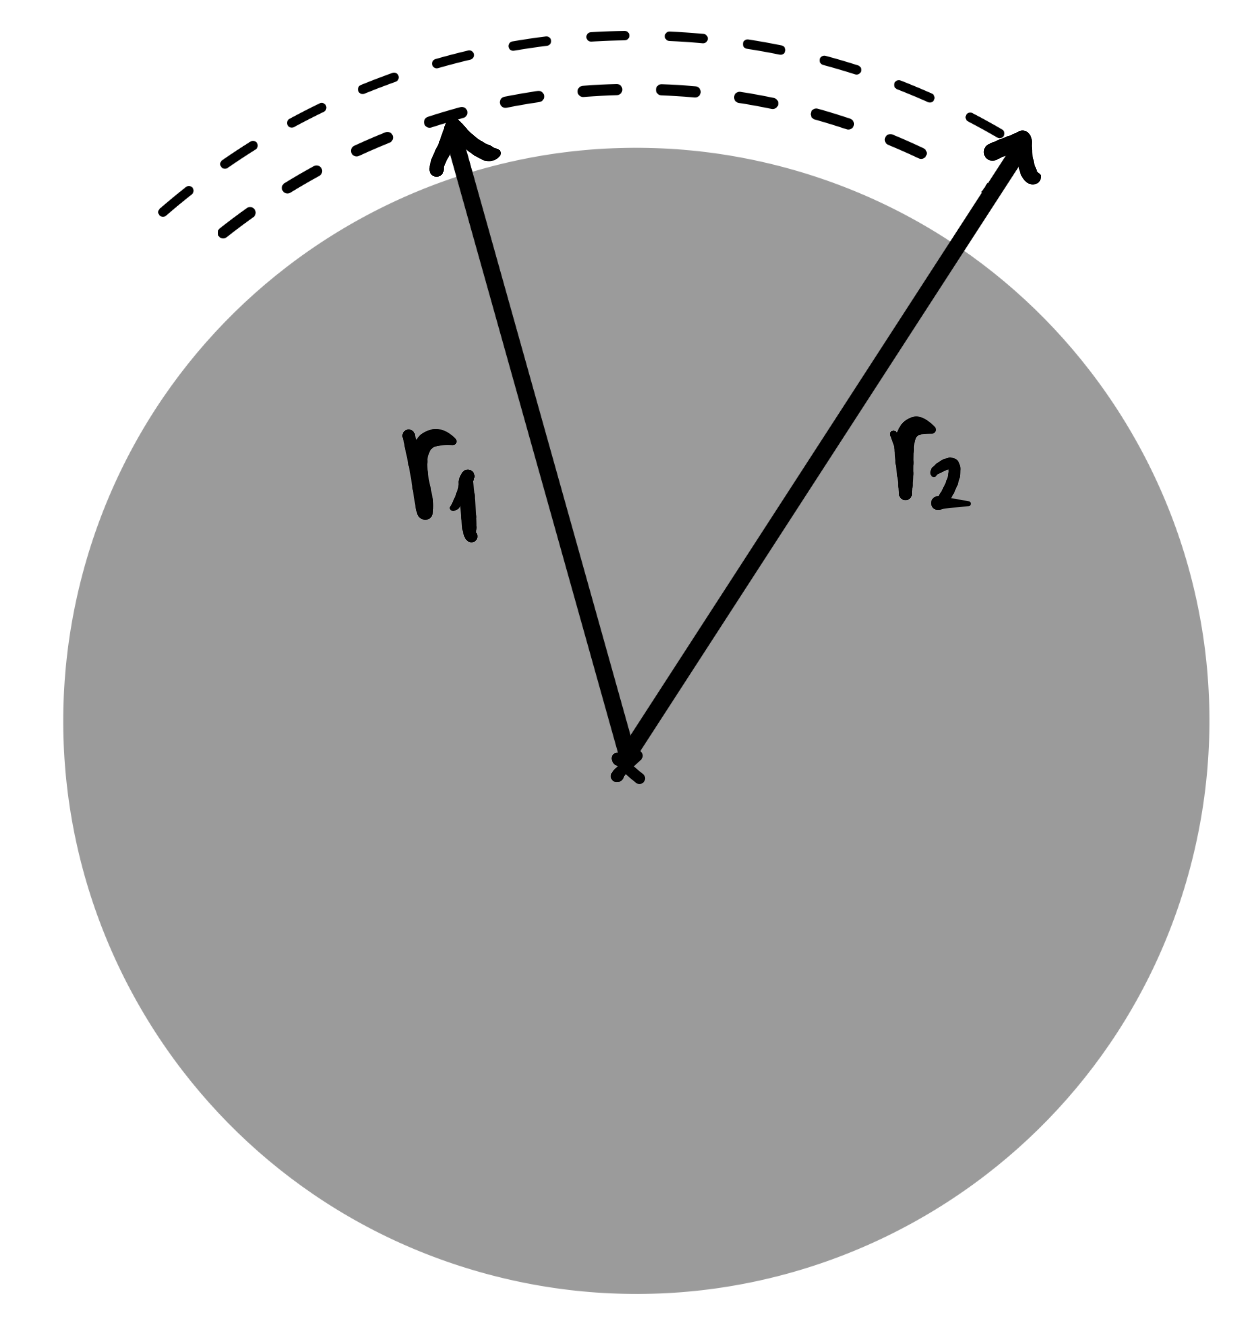
\includegraphics[width=0.25\linewidth]{imagensgravitacao/energiapotencialgravitacional.png}
\captionof{figure}{Duas altitudes bem próximas da superfície da terra, de tal modo que $r_1 \approx r_2 \approx R$.}
\label{fig_newtongravitacao_energiapotencial}
} 
\vspace{0.3cm}

A variação da energia potencial gravitacional sofrida pela pedra neste deslocamento é

$$ \Delta E_P = E_2 - E_1 = -\dfrac{GMm}{r_ 2} - \left(-\dfrac{GMm}{r_1}  \right) = GMm \left( \dfrac{1}{r_1} - \dfrac{1}{r_2} \right) = \dfrac{GMm}{r_1r_2} \left(  r_2 - r_1\right).  $$

Note que o termo entre parênteses é justamente o deslocamento vertical da pedra: $\Delta h = (r_2 - r_1).$ Além do mais, note que o denominador de tal expressão é $r_1\cdot r_2 \approx R^2,$ de tal modo que 

$$  \Delta E_P =  \dfrac{GMm}{R^2} \Delta h = m \cdot  \underbrace{\tikz[baseline=(X.base)] 
\node[draw, dashed, inner sep=2pt] (X) {$\dfrac{GM}{R^2}$};}_{\text{campo g}} \cdot \Delta h = mg \Delta h.$$




Note que o valor $GM/R^2$ representa justamente o valor da aceleração da gravidade na superfície da Terra, de modo que a equação final reduz para o que esperávamos: a variação de energia potencial -- para pontos suficientemente próximos da superfície da Terra -- é dada por $\Delta E_P =  mg \Delta h,$ dependendo, portanto, apenas do desnível vertical $\Delta h$ entre os pontos.

Isso não é uma demonstração da Equação \eqref{eq_newton_energiapotencialgravitacional}. Na verdade, nós partimos de tal equação e demonstramos uma outra, talvez mais familiar ao leitor. Isso talvez seja uma boa evidência da validade da Equação \eqref{eq_newton_energiapotencialgravitacional}: ela é condizente com outra equação que conhecíamos, se reduzindo a ela para casos em que o corpo está próximo da superfície do planeta. 

Isso talvez deixe o leitor um pouco mais confortável -- e também ajude a compreender a relação entre essas diferentes formas de se computar a energia potencial. A Equação \eqref{eq_newton_energiapotencialgravitacional} é a relação geral, porém, ela só precisa ser usada em contextos planetários, em que a distância do corpo à superfície do planeta é relevante. Para corpos na superfície da Terra podemos usar tranquilamente a Equação \eqref{eq_energia_potencialgravitacional}, como demonstrado.



\vspace{0.3cm}



\begin{exemplo}[Nível II]\label{exemplo_gravitacao_energiapotencialgravitacionalex02}
Um satélite de comunicações de massa $m = 2{,}0 \cdot 10^3$ kg é transferido de uma órbita circular baixa de raio $r_1 = 6{,}6 \cdot 10^6$ m para a órbita geoestacionária de raio $r_2 = 4{,}2 \cdot 10^7$ m. Calcule a variação de energia potencial gravitacional nessa transferência.
Dados: $M_T = 6{,}0 \cdot 10^{24}$ kg, $G = 6{,}67 \cdot 10^{-11}$ N{\cdot}m²/kg².

\resolucao

A variação de energia potencial é $\Delta E_p = E_{p,2} - E_{p,1}$.
Calculando cada termo separadamente:

\[
  E_{p,1} = -\frac{GM_T m}{r_1}
          = -\frac{6{,}67\cdot10^{-11} \cdot 6{,}0\cdot10^{24}
                   \cdot 2{,}0\cdot10^3}
                  {6{,}6\cdot10^6}
          \approx -1{,}21\cdot10^{11}\ \text{J}
\]

\[
  E_{p,2} = -\frac{GM_T m}{r_2}
          = -\frac{6{,}67\cdot10^{-11} \cdot 6{,}0\cdot10^{24}
                   \cdot 2{,}0\cdot10^3}
                  {4{,}2\cdot10^7}
          \approx -1{,}90\cdot10^{10}\ \text{J}
\]

\[
  \Delta E_p = E_{p,2} - E_{p,1}
             = -1{,}90\cdot10^{10} - \left(-1{,}21\cdot10^{11}\right)
             \approx \boxed{+1{,}02\cdot10^{11}\ \text{J}}
\]

O resultado positivo significa que o satélite \textit{ganhou} energia
potencial ao subir para a órbita mais alta --- ele saiu de um ponto
mais negativo para um menos negativo, ou seja, subiu no ``buraco''
gravitacional. Essa energia teve que ser fornecida pelos propulsores. Note que essa diferença de energia potencial foi positiva, o que indica que os propulsores tiveram que realizar trabalho, injetando energia no satélite.


\end{exemplo}



\vspace{0.3cm}






\begin{exemplo}[Nível III]\label{exemplo_gravitacao_energiapotencialgravitacionalex03}

Em um sistema binário isolado, duas estrelas de massas $M$ e
$2M$ orbitam o centro de massa comum em órbitas circulares, mantendo
sempre a separação $d$ entre seus centros. Um asteroide de massa
$m \ll M$ gira junto das estrelas, de modo que ele fica em repouso sobre a linha que une as duas, a
uma distância $x$ da estrela de massa $M$.

\begin{enumerate}

  \item[a)] Determine a posição do centro de massa do sistema binário
  (estrela $M$ na origem, estrela $2M$ em $x = d$). Calcule os raios
  orbitais $r_1$ e $r_2$ de cada estrela em torno do CM.

  \item[b)] Mostre que, para que as duas estrelas mantenham órbitas
  circulares com a mesma velocidade angular $\omega$, a força
  gravitacional mútua deve fornecer a força centrípeta de cada uma
  --- e derive a expressão de $\omega$ em função de $G$, $M$ e $d$.

  \item[c)] Determine o ponto $x^*$ sobre a linha entre as estrelas onde 
a força gravitacional resultante sobre o asteroide é nula (ignore a 
contribuição centrípeta do movimento orbital do asteroide).

  \item[d)] Mostre que o equilíbrio em $x^*$ é instável analisando o
  comportamento da força resultante para um pequeno deslocamento
  $\delta$ na direção de $2M$.

  \item[e)] Calcule a energia potencial gravitacional do asteroide em
  $x^*$, em função de $G$, $M$, $m$ e $d$. Mostre que esse ponto é
  um máximo de $E_p$ ao longo da linha, e conecte esse resultado com
  a instabilidade encontrada em (d).

  \item[f)] Por fim, compare $|x^* - x_{CM}|$ com os raios orbitais
  $r_1$ e $r_2$. O ponto de equilíbrio $x^*$ está mais próximo de
  qual estrela? Está dentro ou fora da órbita da estrela menos
  massiva? Interprete fisicamente.

\end{enumerate}



\resolucao

\begin{enumerate}

  \item[a)] Com a estrela $M$ na origem e $2M$ em $x = d$, a posição do centro de massa se dá pela Equação \eqref{eq_newtonrotacao_posicaocentrodemassa}:
  %
  \[
    x_{CM} = \frac{M \cdot 0 + 2M \cdot d}{M + 2M} = \frac{2d}{3}
  \]
  %
  Os raios orbitais são as distâncias de cada estrela ao CM:
  %
  \[
    r_1 = x_{CM} - 0 = \frac{2d}{3},
    \qquad
    r_2 = d - x_{CM} = \frac{d}{3}
  \]
  %
  A estrela menos massiva ($M$) orbita mais longe do CM; a mais
  massiva ($2M$) orbita mais perto --- resultado geral: em um sistema
  binário, massa e raio orbital são inversamente proporcionais.

  \item[b)] Para a estrela $M$, a força gravitacional fornece a resultante
  centrípeta:
  %
  \[
    \frac{GM(2M)}{d^2} = M\omega^2 r_1 = M\omega^2 \cdot \frac{2d}{3}
    \implies
    \omega^2 = \frac{2GM}{d^2} \cdot \frac{3}{2d} = \frac{3GM}{d^3}
  \]
  %
  Verificando para $2M$: 
  
  $$ \dfrac{2GM^2}{d^2} = 2M\omega^2 r_2 ,$$
  
  que fornece $\omega^2 = 3GM/d^3$ --- consistente. Portanto:
  %
  \[
    \boxed{\omega = \sqrt{\frac{3GM}{d^3}}}
  \]
  %
  Esse é o análogo da Terceira Lei de Kepler para o sistema binário:
  $\omega^2 \propto (M_1 + M_2)/d^3$.

  \item[c)] No ponto $x^*$, as atrações das duas estrelas sobre o
  asteroide se cancelam:
  %
  \[
    \frac{GMm}{(x^*)^2} = \frac{2GMm}{(d - x^*)^2}
    \implies
    \frac{(d-x^*)^2}{(x^*)^2} = 2
    \implies
    \frac{d - x^*}{x^*} = \sqrt{2}
  \]
  %
  \[
    \boxed{x^* = \frac{d}{1+\sqrt{2}} = d\!\left(\sqrt{2}-1\right).}
  \]

  \item[d)] Para um deslocamento $\delta > 0$ em direção a $2M$,
  a nova posição é $x^* + \delta$. A força resultante sobre o
  asteroide:
  %
  \[
    F = \frac{GMm}{(x^*+\delta)^2} - \frac{2GMm}{(d-x^*-\delta)^2}
  \]
  %
  O primeiro termo diminui (denominador maior); o segundo aumenta
  (denominador menor). O resultado líquido aponta na direção de
  $2M$ --- mesma direção do deslocamento. A força não é restauradora:
  o equilíbrio é instável.

  \item[e)] A energia potencial em $x^*$:
  %
  \[
    E_p(x^*) = -\frac{GMm}{x^*} - \frac{2GMm}{d - x^*}
  \]
  %
  Substituindo $x^* = d(\sqrt{2}-1)$, portanto
  $d - x^* = d(2 - \sqrt{2})$ e racionalizando, teremos

  \[
    E_p(x^*)
    = -\frac{GMm}{d}\!\left[(\sqrt{2}+1) + (2+\sqrt{2})\right]
    = -\frac{GMm}{d}\!\left(3 + 2\sqrt{2}\right)
  \]
  %
  Nas vizinhanças de $x^*$, a proximidade de qualquer uma das
  estrelas torna $E_p$ muito mais negativa --- portanto $x^*$ é um
  \textbf{máximo} de $E_p$ ao longo da linha. Máximo de energia
  potencial significa mínimo de estabilidade: qualquer deslocamento
  libera energia cinética e afasta o asteroide do ponto de
  equilíbrio, em coerência com a análise de forças de~(d).

  \item[f)] O ponto de equilíbrio está em
  $x^* \approx 0{,}414\,d$ e o CM em $x_{CM} = 2d/3 \approx
  0{,}667\,d$. A distância entre eles:
  %
  \[
    |x^* - x_{CM}|
    = \left|d(\sqrt{2}-1) - \frac{2d}{3}\right|
    = d\left|\sqrt{2} - \frac{5}{3}\right|
    \approx 0{,}253\,d
  \]
  %
  Como $r_1 = 2d/3 \approx 0{,}667\,d$, temos
  $|x^* - x_{CM}| < r_1$: o ponto de equilíbrio está
  \textbf{dentro} da órbita da estrela menos massiva, entre ela
  e o CM.

  Fisicamente, isso faz sentido: $x^*$ é o ponto onde a atração
  da estrela próxima ($M$, à esquerda) e a da estrela distante e
  mais massiva ($2M$, à direita) se equilibram. Como $2M$ é mais
  forte mas está mais longe, o equilíbrio se desloca para perto
  de $M$ --- mas não tanto a ponto de sair da região entre as
  duas estrelas. O asteroide nesse ponto está, por assim dizer,
  no cume energético entre dois poços gravitacionais: qualquer
  perturbação o lança irreversivelmente em direção a um dos dois.

\end{enumerate}

\end{exemplo}









\begin{secnivel}[Velocidade de Escape]{II}{Velocidade de Escape}
 

\eqLdois{dem}{eq_newton_velocidadeescape}{v_\text{E} = \sqrt{\dfrac{2GM}{R}}}
  
\end{secnivel}


\secgfe{De onde vem}

A velocidade de escape de um corpo equivale a menor velocidade com a qual ele deve ser lançado da superfície de um planeta esférico de massa $M$ e raio $R$ a fim de que ele consiga escapar do campo gravitacional de tal planeta. Na Equação \eqref{eq_newton_velocidadeescape}, $G$ é a constante de gravitação universal.

Quando dizemos que ele conseguirá escapar da gravidade de tal planeta, significa que ele não executará uma órbita fechada, no caso, circular ou elíptica. Ele possui velocidade suficiente para se desprender do campo gravitacional e entrar em uma trajetória que não é orbital: ele conseguirá se afastar infinitamente do planeta.

Sendo assim, o corpo, ao estar infinitamente longe, ainda terá alguma velocidade, ainda que seja totalmente desacelerado pelo planeta. Equacionando a conservação da energia mecânica do corpo no ponto em que ele foi lançado (na superfície do planeta) e quando ele está infinitamente longe dele, teremos:

\begin{align}
    E_{\text{M}_\text{SUPERFÍCIE}} &=  E_{\text{M}_{\infty}} \nonumber \\
    \dfrac{1}{2}mv_\text{E}^2 + \left( - \dfrac{GMm}{R}\right) &= \dfrac{1}{2}m v_{\infty}^2, \nonumber 
\end{align}

\noindent em que $v_{\infty}$ representa o valor de velocidade com que este corpo chega ``no infinito.'' Note que, no infinito, a influência do campo gravitacional do planeta é desprezível, de modo que a energia potencial gravitacional entre o corpo e o planeta é nula -- essa é a razão de não haver este termo no segundo membro da equação.

Logo, teremos, desenvolvendo:

$$ \dfrac{1}{2}mv_\text{E}^2  - \dfrac{GMm}{R} = \dfrac{1}{2}m v_{\infty}^2  \implies  v_\text{E}^2 = \dfrac{2GM}{R} + v_{\infty}^2. $$

Note que existem infinitos valores de velocidade que este corpo pode ter ao chegar no infinito, todos eles dependendo, naturalmente, do valor da velocidade $v_\text{E}$ com que o corpo foi lançado na superfície do planeta. Quanto maior a velocidade com que este corpo for lançado, maior será o valor de velocidade que ``sobrará'' ao corpo quando ele chegar no infinito. Sendo assim, no caso de considerarmos a \textbf{menor velocidade} com que o corpo deve ser lançado, ele chegará no infinito quase parando: ele tinha exatamente a velocidade suficiente para escapar do campo gravitacional, sendo praticamente totalmente desacelerado pela gravidade do planeta ao longo da sua trajetória.

Assim, a menor velocidade com que o corpo é lançado é aquela para a qual $ v_{\infty}\approx 0,$ ou seja:

$$ v_\text{E}^2 = \dfrac{2GM}{R} + \cancelto{0}{v_{\infty}^2} \implies \boxed{v_\text{E} = \sqrt{\dfrac{2GM}{R}},} $$

\noindent como expressa a Equação \eqref{eq_newton_velocidadeescape}.

\secgfe{Onde é usada} 

O contexto aqui é direto e sem muita margem para dúvida: a Equação \eqref{eq_newton_velocidadeescape} se aplica no contexto de gravitação, especificamente para computar a velocidade que um corpo deve ter, sendo lançado da superfície do planeta de raio $R,$ para fugir do campo gravitacional daquele planeta.

Quaisquer velocidades superiores àquela, naturalmente, farão o corpo se desprender do campo gravitacional do planeta e se afastar infinitamente dele.

\secgfe{Erros comuns}


É comum que o aluno confunda as Equações \eqref{eq_gravitacao_velocidadeorbital} e \eqref{eq_newton_velocidadeescape}. Contudo, apesar das expressões serem bem semelhantes, tratam-se de duas velocidades completamente diferentes. A primeira se trata da velocidade $v_o$ que um corpo deve ter para estar confinado no campo gravitacional do planeta de massa $M$, executando a órbita de raio $r=R+h.$ Já a segunda se trata da menor velocidade que este mesmo corpo deve ter para ser lançado para fora do planeta e nunca mais voltar: ele terá velocidade suficiente para não ficar preso em uma órbita e escapar do campo gravitacional deste planeta.

É interessante notar que a velocidade de escape não é tão maior assim do que a velocidade orbital. Considerando um satélite que orbita tangenciando a superfície da terra, teremos, na Equação \eqref{eq_gravitacao_velocidadeorbital}, $h \approx 0.$ Desse modo, a razão entre a velocidade $v_\text{E}$ com que o corpo deve ser lançado da superfície deste planeta para nunca mais voltar e a velocidade $v_o$ que ele deve ter para orbitar tangenciando a superfície do planeta é

$$ \dfrac{v_\text{E}}{v_o} = \dfrac{\sqrt{ \dfrac{2GM}{R}}}{\sqrt{\dfrac{GM}{R}}} = \sqrt 2 \approx 1.41.$$

Ou seja, para escapar da gravidade do planeta, basta uma velocidade 41\% maior do que a necessária para permanecer em órbita na mesma altitude. Para o caso do planeta Terra, a velocidade de escape é

$$ v_\text{E} = \sqrt{\dfrac{2GM}{R}} = \sqrt{\dfrac{2 \cdot 6.67 \cdot 10^{-11} \cdot 6 \cdot 10^{24}}{6400 \cdot 10^3}} \approx 11.200  \text{ m/s} =  \boxed{40.000 \text{ km/h.}} $$



\secgfe{Observações}

% Falar da trajetória gravitacaoconicas
% + desenho mostrando a elipse virando parábola.

Há uma pergunta aparentemente simples, mas cuja resposta envolve complexos desdobramentos matemáticos: quando um objeto é lançado com a velocidade de escape, que forma tem a sua
trajetória?
 
 
A resposta é uma \textit{parábola}. E para entender por que, precisamos fazer um
pequeno desvio pela geometria.
 

Imagine um cone duplo --- dois cones com o mesmo vértice, abertos para direções
opostas, como uma ampulheta de arestas retas. Agora imagine um plano cortando esse
cone em diferentes ângulos, como na Figura \ref{fig_gravitacao_gravitacaoconicas}. Dependendo da inclinação do corte, a interseção do plano
com o cone produz curvas radicalmente diferentes:
 
\begin{itemize}
  \item Um corte \textit{fechado} (quase horizontal) produz uma \textit{elipse} ---
    ou, no caso extremo de ser perfeitamente horizontal, um círculo.
  \item Um corte \textit{paralelo a uma das arestas} do cone produz uma
    \textit{parábola}.
  \item Um corte \textit{mais inclinado ainda}, que atravessa os dois cones, produz
    uma \textit{hipérbole}.
\end{itemize}

\vspace{0.3cm}
{
\centering
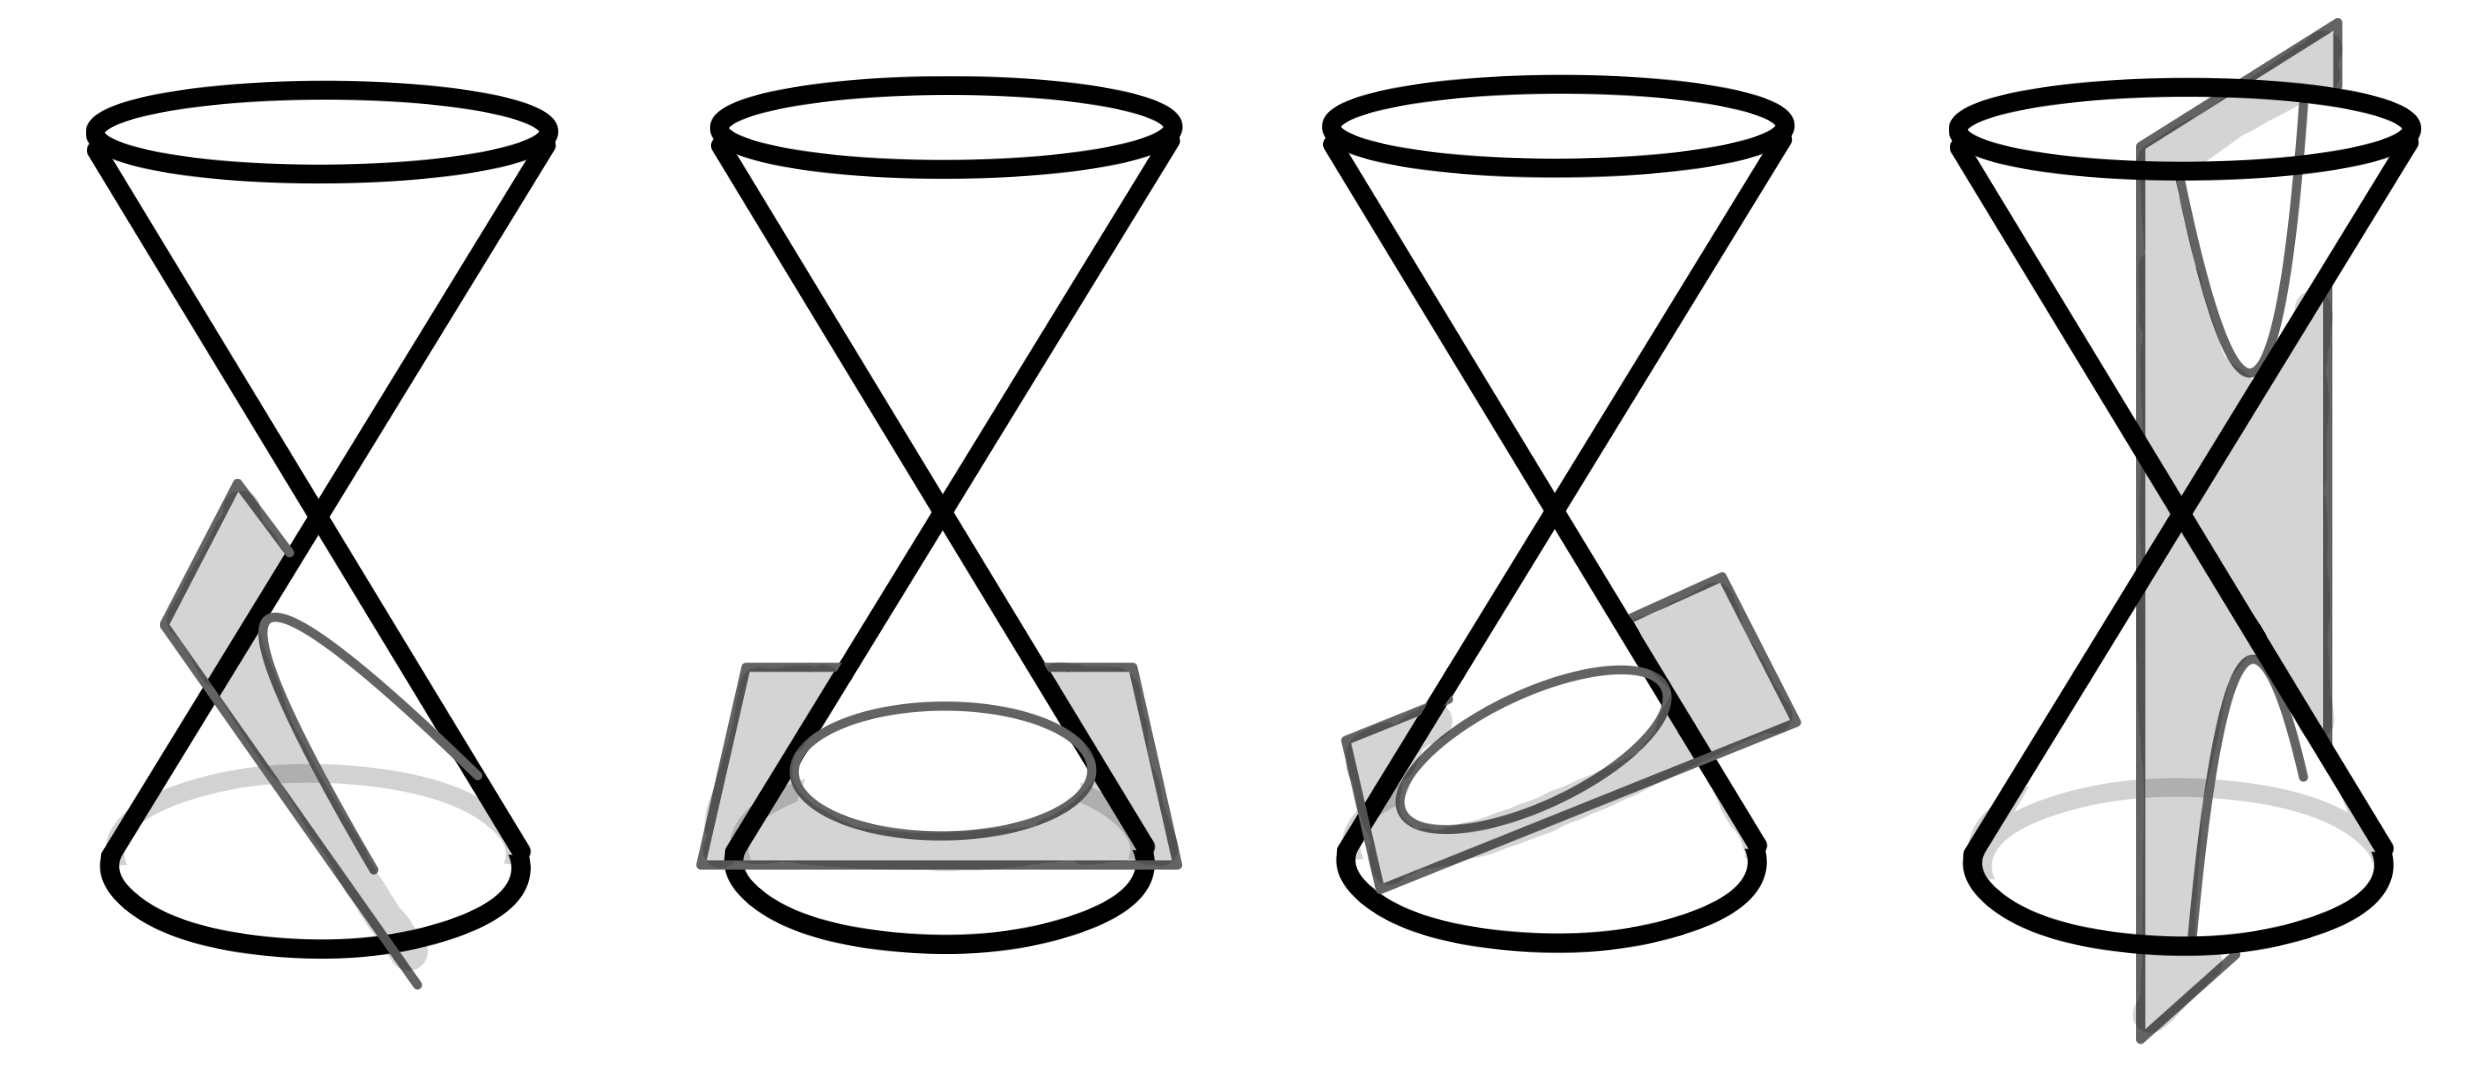
\includegraphics[width=0.6\linewidth]{imagensgravitacao/gravitacaoconicas.png}
\captionof{figure}{Parábola, circunferência, elipse e hipérbole: as respectivas secções cônicas.}
\label{fig_gravitacao_gravitacaoconicas}
} 
\vspace{0.3cm}
 
Essas quatro curvas --- círculo, elipse, parábola, hipérbole --- são chamadas de
\textit{cônicas}, e os geômetras gregos as estudavam com paixão há mais de dois mil
anos, muito antes de qualquer ideia de gravitação.
 
A conexão entre elas veio com Newton. No \textit{Principia Mathematica} (1687), Newton
demonstrou algo que nenhum grego poderia ter imaginado: \textit{toda trajetória
gravitacional é uma cônica, com o corpo central em um dos focos.} Não algumas
trajetórias --- todas. Planetas em órbita, cometas de passagem, foguetes lançados da
Terra, asteroides capturados pelo Sol: sem exceção, cada um deles percorre uma elipse,
uma parábola ou uma hipérbole.\footnote{A demonstração de Newton é um dos resultados
mais belos de toda a física matemática. Ela conecta a lei do inverso do quadrado da
distância --- $F \propto 1/r^2$ --- à geometria das cônicas, resultado que os gregos
desenvolveram por razões puramente estéticas dois milênios antes. Que a natureza usasse
exatamente essas curvas não era óbvio para ninguém até Newton.}
 
O que determina qual cônica um objeto percorre? A resposta é a velocidade de
lançamento. Imagine que você está na superfície de um planeta sem atmosfera e lança um
objeto horizontalmente, aumentando progressivamente a velocidade:
 
Com velocidade baixa, o objeto segue uma trajetória que, levando em conta a curvatura
do planeta, é uma \textit{elipse} tão excêntrica que intersecta o chão. Sua impressão é de que essa trajetória é parabólica, como mostra a primeira imagem da Figura \ref{fig_gravitacao_gravitacaotrajetoriasconicas}. Contudo, essa impressão se dá porque, olhando bem de perto, uma parábola parece muito com uma elipse. Na verdade qualquer curva pode ser aproximada, em primeira instância, por uma parábola, olhando suficientemente de perto. A segunda imagem da figura evidencia isso, enquanto a terceira imagem destaca o que ocorre de fato: a trajetória que achamos ser parabólica é na verdade elíptica, com o centro da Terra em um dos focos dessa elipse.



\vspace{0.3cm}
{
\centering
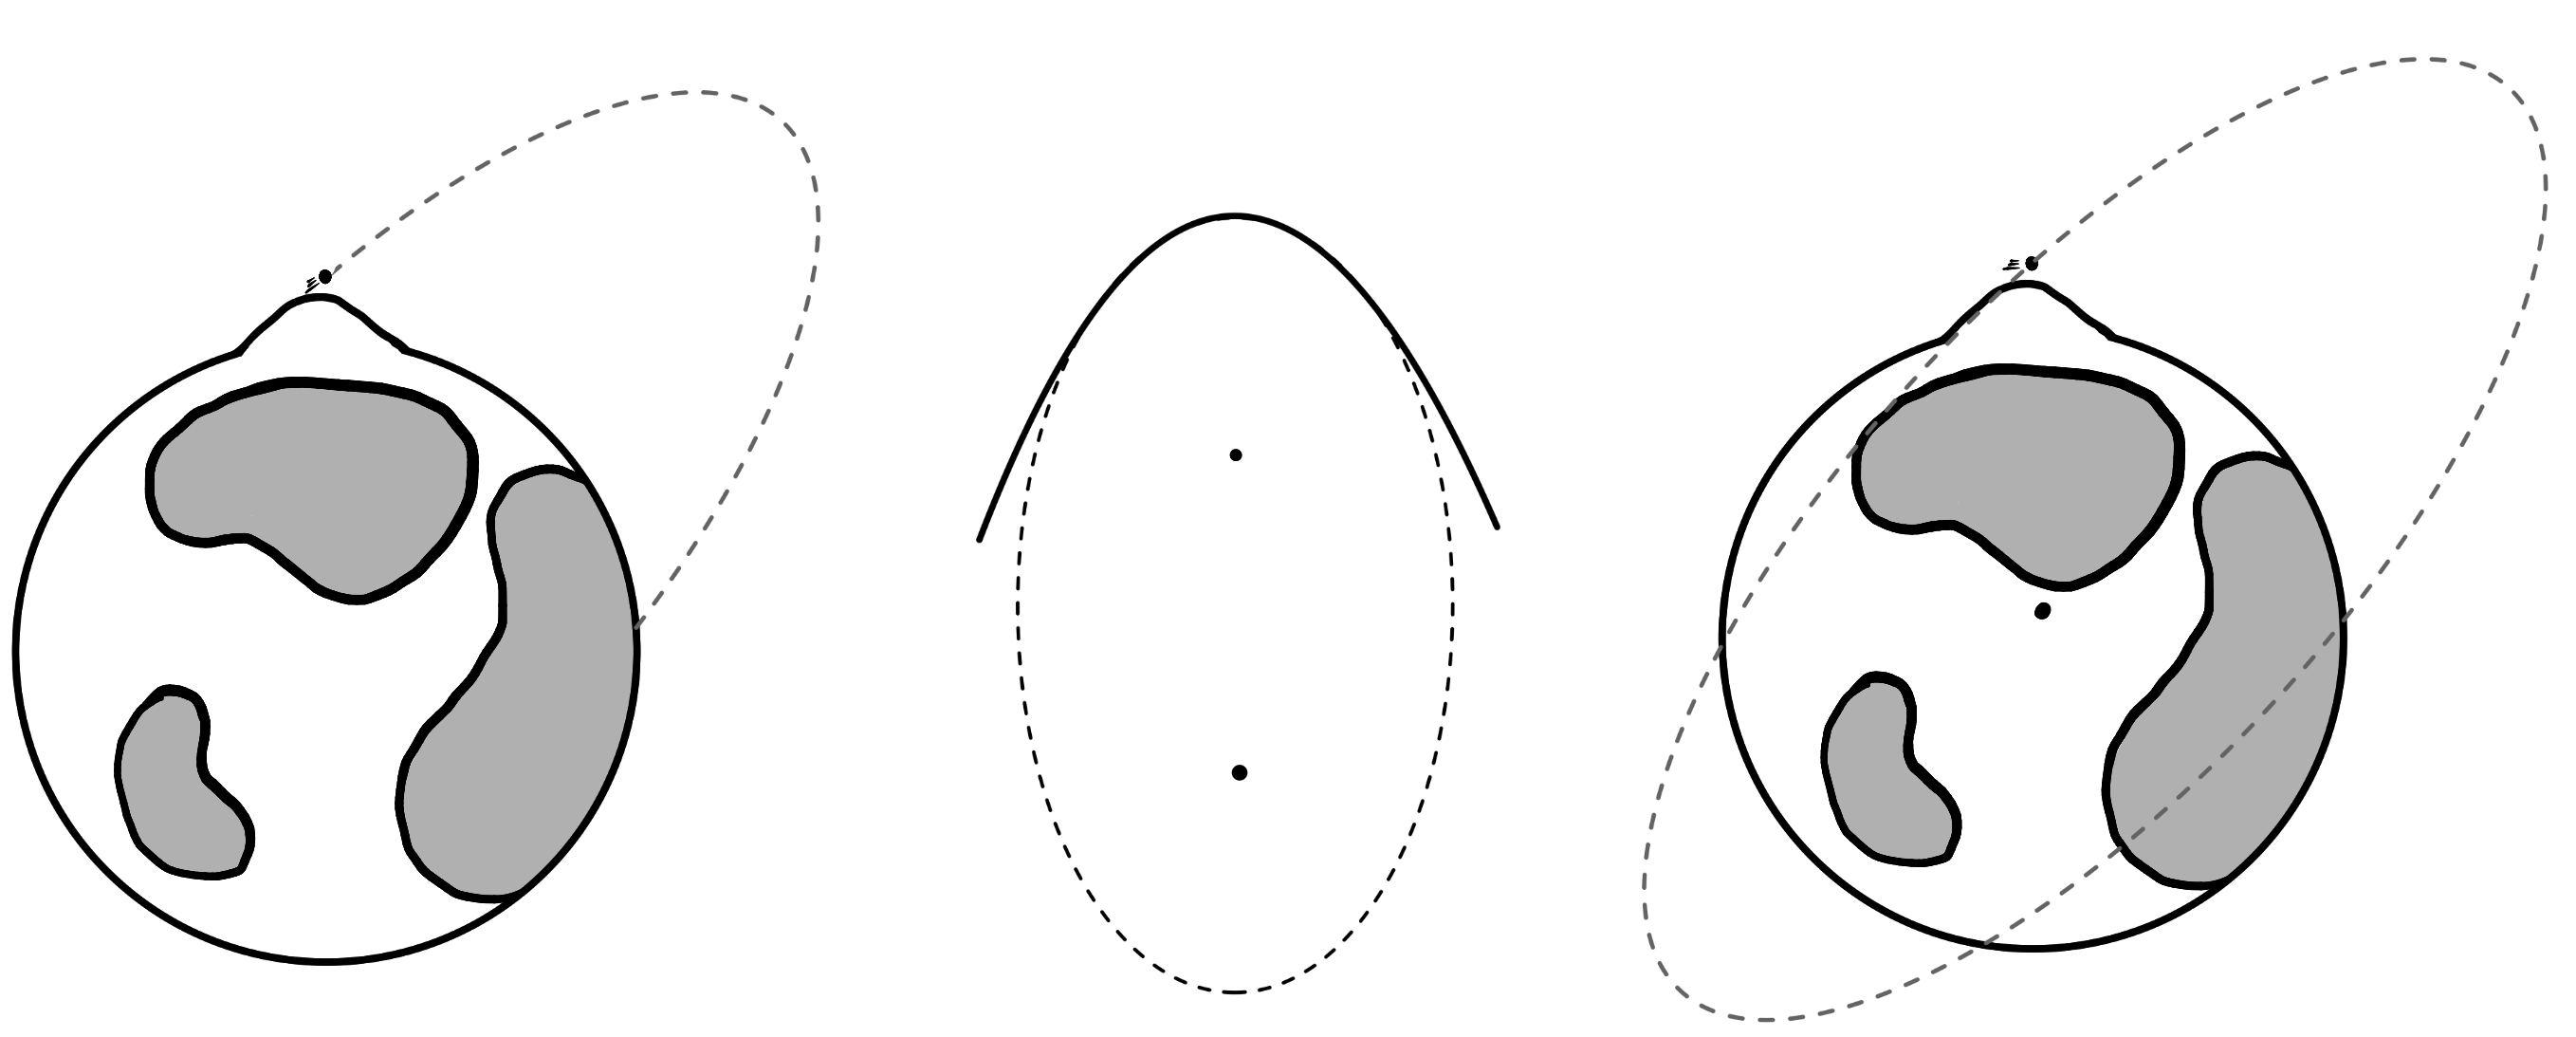
\includegraphics[width=0.75\linewidth]{imagensgravitacao/gravitacaotrajetoriasconicas.png}
\captionof{figure}{Toda curva é, olhando de muito perto, uma parábola.}
\label{fig_gravitacao_gravitacaotrajetoriasconicas}
} 
\vspace{0.3cm}


Aumentando a velocidade, a elipse se alonga. Com a velocidade orbital certa, ela se fecha
perfeitamente ao redor do planeta --- o objeto entra em \textit{órbita circular}. Com
velocidades entre a orbital e a de escape, as órbitas são \textit{elipses mais abertas}.
 
Quando a velocidade atinge exatamente $v_e$, algo muda qualitativamente: a elipse se
abre tanto que nunca mais fecha. A trajetória se torna uma \textit{parábola} --- uma
curva que, diferentemente da elipse, não retorna jamais ao ponto de partida. Portanto, sempre que um objeto for lançado \emph{exatamente} com a velocidade de escape, sua trajetória será parabólica.
 
Com velocidade superior a $v_e$, a trajetória é uma \textit{hipérbole}: o objeto
escapa com energia sobrando, e passa pelo campo gravitacional do planeta como um
viajante que atravessa uma cidade sem parar.
 






\vspace{0.3cm}



\begin{exemplo}[Nível II (ITA 1991)]\label{exemplo_gravitacao_velocidadedeescapeex02}

Considere um planeta cuja massa é o triplo da massa da Terra e seu raio, o dobro do raio da Terra. Determine a relação entre a velocidade de escape deste planeta e a da Terra $(v_P/v_T)$ e a relação entre a aceleração gravitacional na superfície do planeta e a da Terra $(g_P/g_T)$.

\vspace{0.5cm}

\begin{enumerate}
    \item[(a)] $\dfrac{v_P}{v_T}=\sqrt{\dfrac{3}{4}} \;\text{e}\; \dfrac{g_P}{g_T}=\dfrac{3}{4}$
    
    \item[(b)] $\dfrac{v_P}{v_T}=\sqrt{\dfrac{3}{2}} \;\text{e}\; \dfrac{g_P}{g_T}=\dfrac{3}{4}$
    
    \item[(c)] $\dfrac{v_P}{v_T}=\sqrt{\dfrac{3}{2}} \;\text{e}\; \dfrac{g_P}{g_T}=\dfrac{3}{2}$
    
    \item[(d)] $\dfrac{v_P}{v_T}=\dfrac{3}{2} \;\text{e}\; \dfrac{g_P}{g_T}=\dfrac{3}{4}$
    
    \item[(e)] n.d.a.
\end{enumerate}

\resolucao

A relação entre as acelerações gravitacionais são dadas pela Equação \eqref{eq_newton_campogravitacional}:

$$ \dfrac{g_P}{g_T} = \dfrac{\dfrac{G(3M_T)}{(2R_T)^2}}{\dfrac{GM_T}{R_T^2}} = \dfrac{3}{4}.$$

Já a razão entre as velocidades de escape é

$$ \dfrac{v_P}{v_T} = \dfrac{\sqrt{\dfrac{2G(3M_T)}{2R_T}}}{\sqrt{\dfrac{2GM_T}{R_T}}} = \sqrt{\dfrac{3}{2}},$$

\noindent de modo que a resposta é a alternativa B.


\end{exemplo}





\vspace{0.3cm}




\begin{exemplo}[Nível III]\label{exemplo_gravitacao_velocidadedeescapeex03}

Dado um planeta esférico de raio $R$ e de massa $M$, de quanto deveríamos comprimi-lo a fim de que ele se torne um buraco negro?


\resolucao

Um buraco negro é um corpo para o qual $v_\text{E} > c,$ em que $c$ é a velocidade da luz. Ou seja, nem mesmo a luz -- que se move na maior velocidade que existe no universo -- é capaz de escapar do campo gravitacional de tal corpo, a partir de sua superfície. Usando a Equação \eqref{eq_newton_velocidadeescape}, teremos

$$ v_\text{E} > c \implies \sqrt{\dfrac{2GM}{R}} > c \implies \dfrac{2GM}{R}> c^2 \implies \boxed{R < \dfrac{2GM}{c^2}.} $$

Ou seja, toda a massa $M$ do planeta deve estar condensada em uma esfera de raio $r<r_s$ tal que 

$$ r_s = \dfrac{2GM}{c^2},$$

\noindent conhecido como raio de Schwarzschild. 

% Assim, considerando o caso limite, em que toda a massa do planeta será condensada em uma esfera de raio $r=r_s,$ a razão entre o raio inicial do planeta e o seu novo raio, para que ele se torne um buraco negro, é 

% $$ \dfrac{R}{r_s} = \dfrac{R}{ \dfrac{2GM}{c^2}}.$$

A título de exemplo, usando a massa da Terra, o seu raio de Schwarzschild dado pela equação acima seria de apenas 9 milímetros. Isso mesmo, seria necessário condensar toda a massa da Terra em uma esfera do tamanho de uma bola de gude para que o campo gravitacional fosse tão intenso a ponto de que nem a luz seria capaz de escapar quando passasse tangenciando a sua superfície: isso é um buraco negro.

\end{exemplo}


\vspace{0.3cm}
















\begin{secnivel}[Energia Orbital Total]{III}{Energia Orbital Total}
 

\eqLdois{dem}{eq_newton_energiaorbitaltotal}{E = -\dfrac{GMm}{2a}}
  
\end{secnivel}


\secgfe{De onde vem}

A Equação \eqref{eq_newton_energiaorbitaltotal} fornece qual é a energia mecânica total (a soma da energia cinética com a potencial gravitacional) de um satélite de massa $m$ que está orbitando um astro de massa $M$, em uma órbita elíptica de eixo maior $2a$. Em tal equação $G$ é a constante de gravitação universal.

\vspace{0.3cm}
{
\centering
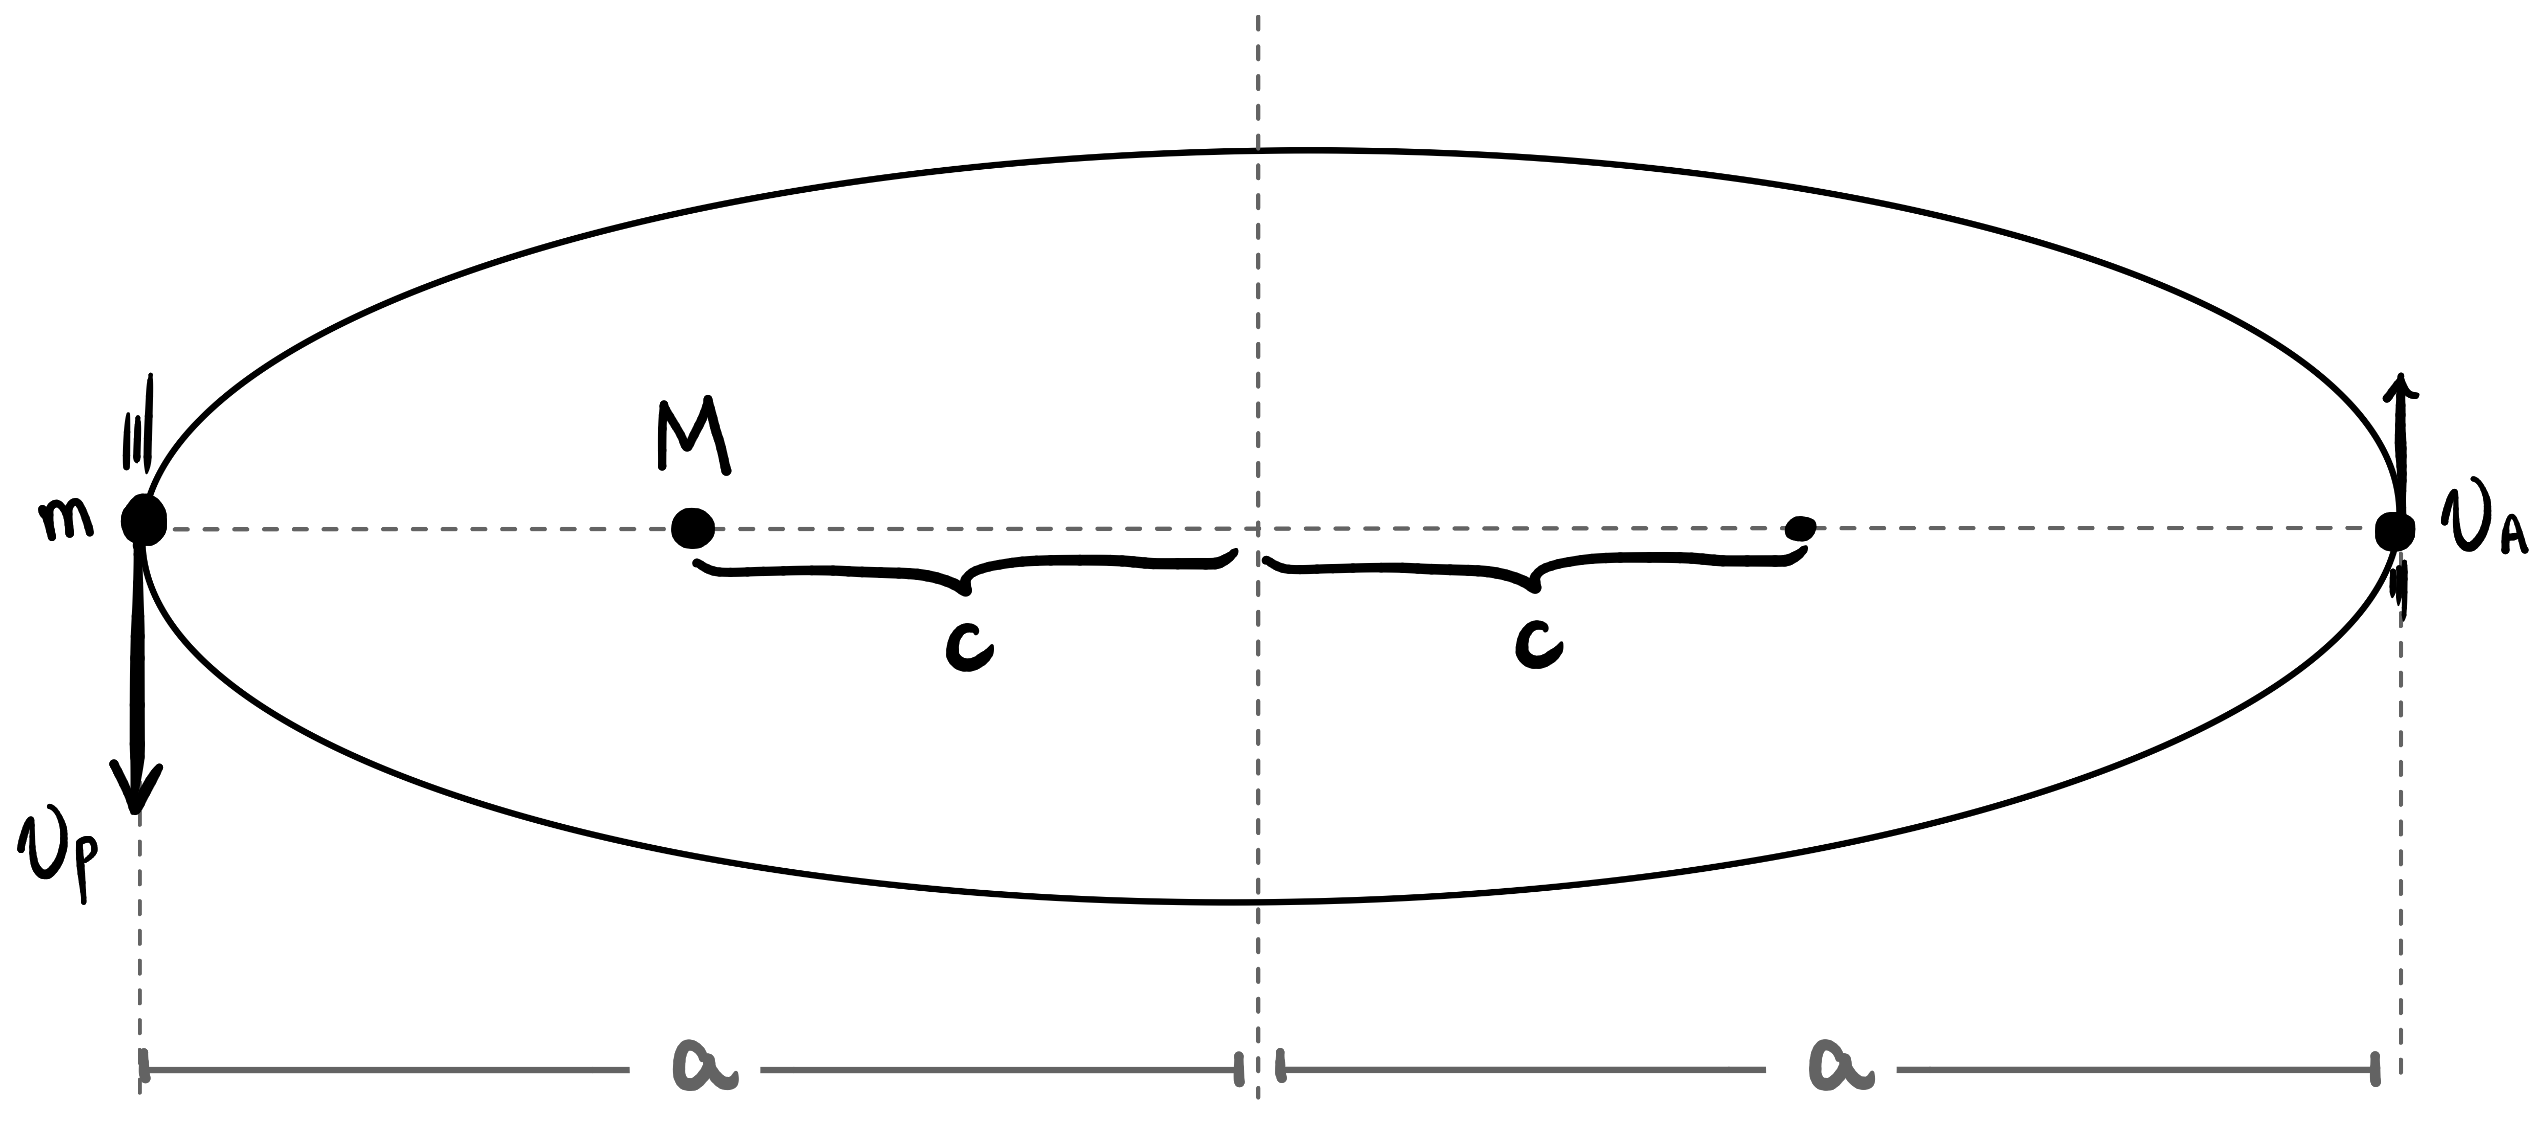
\includegraphics[width=0.6\linewidth]{imagensgravitacao/energiaorbitaltotalgravitacao.png}
\captionof{figure}{Satélite em órbita elíptica e conservação do momento angular.}
\label{fig_gravitacao_energiaorbitaltotalgravitacao}
} 
\vspace{0.3cm}


Em um movimento sob a ação da força gravitacional o momento angular da partícula é conservado, conforme discutido no desenvolvimento da Equação \eqref{eq_momento_angular}. Desse modo, podemos escolher dois pontos específicos, digamos o ponto $A$, no qual a partícula está o mais afastada possível da massa $M$ (afélio), e o ponto $P,$ no qual a partícula está o mais próxima possível da massa $M$. A Figura \ref{fig_gravitacao_energiaorbitaltotalgravitacao} mostra esses dois pontos, em que $c$ é a distância focal e $a$ é o semi-eixo maior da elipse.

Podemos escrever, para cada um deles, a expressão para a energia mecânica total da partícula em cada um desses pontos -- que terá o mesmo valor, tendo em vista que força gravitacional é conservativa:

\begin{align}
    E &=  \dfrac{1}{2}mv_\text{A}^2 + \left( - \dfrac{GMm}{a+c} \right) \nonumber \\
    E &=  \dfrac{1}{2}mv_\text{P}^2 + \left( - \dfrac{GMm}{a-c} \right). \nonumber
\end{align}

De tais relações, podemos isolar as velocidades e dividir uma equação pela outra, o que nos leva a

$$ \dfrac{v_\text{A}^2}{v_\text{P}^2} = \dfrac{E + \dfrac{GMm}{a+c} }{E + \dfrac{GMm}{a-c}}.$$



A segunda lei de Kepler é equivalente a exigir que o momento angular $L$ da partícula se conserve sob a ação da força gravitacional.\footnote{Revisite o estudo da Equação \eqref{eq_momento_angular} caso não tenha compreendido essa afirmação.} Sendo assim, usando a Equação \eqref{eq_momento_angular} e impondo tal condição, teremos, para os pontos $A$ e $P$:

\begin{align}
    L_\text{A} &=  L_\text{P} \nonumber \\
    mv_\text{A}r_\text{A} \sin \left( \dfrac{\pi}{2} \right) &=   mv_\text{P}r_\text{P} \sin \left( \dfrac{\pi}{2} \right) \nonumber \\
    v_\text{A} (a+c) & = v_\text{P} (a-c), \nonumber
\end{align}

\noindent de onde segue que a razão entre as velocidades $v_\text{A}$ e $v_\text{P}$ é $\sfrac{(a-c)}{(a+c),}$ o que, na equação obtida das expressões da energia total, nos leva a


$$ \dfrac{(a-c)^2}{(a+c)^2} = \dfrac{E + \dfrac{GMm}{a+c} }{E + \dfrac{GMm}{a-c}}.$$

Isolando a energia total $E$ na expressão acima chega-se na Equação \eqref{eq_newton_energiaorbitaltotal}.



% Considere que tal satélite está em um ponto qualquer de sua órbita, distando $r$ da massa $M$. Neste caso, sua energia mecânica em tal ponto arbitrário é

% $$ E = \dfrac{1}{2}mv^2 + \left( - \dfrac{GMm}{r} \right),$$

% \noindent em que $v$ é a velocidade do satélite nesse ponto.


\secgfe{Onde é usada}

Em problemas de gravitação nos quais um corpo está confinado em um órbita elíptica (ou circular)\footnote{Em caso de uma órbita circular de raio $R,$ usamos $2a=2R$ na Equação \eqref{eq_newton_energiaorbitaltotal}, o que é bem razoável: o eixo maior de uma circunferência é o seu diâmetro.} em torno de outro. 

Considere por exemplo que é conhecido o eixo maior $2a$ da órbita elíptica de um satélite de massa $m$ em torno de um planeta de massa $M.$ Neste caso, considere o problema de encontrar em quais pontos de sua órbita ele possui uma dada velocidade $v$. Ora, para qualquer ponto de sua órbita no qual ele esteja a uma distância $r$ do planeta de massa $M$, sua energia total será

$$ E = \dfrac{1}{2}mv^2 + \left( - \dfrac{GMm}{r} \right). $$

Contudo, pela Equação \eqref{eq_newton_energiaorbitaltotal}, sabemos que em qualquer ponto que computarmos sua energia mecânica ela deve dar sempre $\sfrac{-GMm}{(2a)}$, de tal modo que

$$ E = \dfrac{1}{2}mv^2 + \left( - \dfrac{GMm}{r} \right) = -\dfrac{GMm}{2a}. $$

Da expressão acima podemos obter $v(r)$ ou $r(v),$ isto é, funções que forneçam a velocidade do satélite em termos da sua posição $r,$ ou sua inversa. No caso em questão, poderíamos isolar $r$ e obter que

$$ r(v) = \frac{2GM}{v^2 + \frac{GM}{a}}, $$

\noindent ou seja, dado um valor de $v$, podemos descobrir qual é a posição do satélite $r$ em relação ao planeta de massa $M$ na qual ele possui aquela velocidade.


\secgfe{Erros comuns}

A Equação \eqref{eq_newton_energiaorbitaltotal} pressupõe que a força gravitacional é a única que atua no satélite. Assim, caso o satélite ligue algum sistema de propulsão, sua energia cinética irá aumentar (ou diminuir) devido a uma força que não é gravitacional, o que fará variar a sua energia mecânica total (e, consequentemente, afetar a sua órbita). 

É preciso ter cuidado, portanto, para garantir que o satélite está se movendo exclusivamente sob a ação da força gravitacional a fim de aplicar a Equação \eqref{eq_newton_energiaorbitaltotal}.


\secgfe{Observações}


Perceba que, em qualquer ponto da órbita do satélite, sua energia mecânica total será a soma de um termo positivo e um termo negativo:

$$ E = \underbrace{ E_\text{CINÉTICA}}_{\text{positiva}} +  \underbrace{ E_\text{POTENCIAL}}_{\text{negativa}}.$$

Sendo assim, todos os estados que resultarem em uma energia total negativa são aqueles nos quais o termo de energia potencial é predominante: a energia potencial é maior (em módulo) do que a energia cinética. Isso faz com que o satélite esteja confinado naquele campo gravitacional, e as órbitas de energia total negativa são, portanto, fechadas, representando um estado em que o satélite está ``aprisionado.''

Desse modo, é natural que a energia total de um satélite em uma órbita elíptica, que é o que expressa a Equação \eqref{eq_newton_energiaorbitaltotal}, seja negativa. 

O primeiro estado em que o satélite estaria ``livre'' seria aquele no qual $E=0,$ ou seja, há energia cinética suficiente para igualar à energia potencial, de modo que o satélite consegue escapar daquele campo gravitacional e não fica confinado. A trajetória resultante desse estado é parabólica, e trata-se exatamente da situação descrita pela Equação \eqref{eq_newton_velocidadeescape}.

\vspace{0.3cm}

\begin{exemplo}[Nível III (ITA - 2015)]\label{exemplo_gravitacao_velocidadedeescapeex03}

Uma nave espacial segue inicialmente uma trajetória circular de raio $r_A$ em torno da Terra. Para que a nave percorra uma nova órbita também circular, de raio $r_B > r_A$, é necessário por razões de economia fazer com que ela percorra antes uma trajetória semielíptica, denominada órbita de transferência de Hohmann, mostrada na figura.

\vspace{0.3cm}

\begin{center}
\begin{tikzpicture}[scale=0.6, line cap=round, line join=round]

    % Parâmetros
    \def\rA{1.55}
    \def\rB{3.35}
    \pgfmathsetmacro{\a}{(\rA+\rB)/2}      % semi-eixo maior
    \pgfmathsetmacro{\c}{(\rB-\rA)/2}      % distância centro-foco
    \pgfmathsetmacro{\b}{sqrt(\a*\a-\c*\c)}% semi-eixo menor

    % Terra no foco
    \coordinate (O) at (0,0);

    % Centro da elipse
    \coordinate (C) at (-\c,0);

    % Pontos extremos
    \coordinate (A) at (\rA,0);
    \coordinate (B) at (-\rB,0);

    % Órbitas circulares
    \draw (O) circle (\rA);
    \draw (O) circle (\rB);

    % Elipse de transferência
    \draw (C) ellipse ({\a} and {\b});

    % Diâmetro horizontal
    \draw (B) -- (A);

    % Terra
    \fill (O) circle (1.1pt);

    % Vetores velocidade
    \draw[->] (A) -- ++(0,0.95);
    \node[right] at ($(A)+(0,0.95)$) {$v_A$};

    \draw[->] (B) -- ++(0,-0.95);
    \node[left] at ($(B)+(0,-0.95)$) {$v_B$};

    % Rótulos dos pontos
    \node[right] at (A) {$A$};
    \node[left] at (B) {$B$};

    % Rótulo r_A
    \node[below] at ($(O)!0.57!(A)$) {$r_A$};

    % Rótulo r_B deslocado para não cruzar a órbita interna
    \node[above] at ($(B)!0.23!(O)$) {$r_B$};

\end{tikzpicture}
\end{center}

\vspace{0.3cm}

Para tanto, são fornecidos à nave dois impulsos, a saber: no ponto $A$, ao iniciar sua órbita de transferência, e, no ponto $B$, ao iniciar sua outra órbita circular.

Sendo $M$ a massa da Terra; $G$, a constante de gravitação universal; $m$ e $v$, respectivamente, a massa e a velocidade da nave; e constante a grandeza $mrv$ na órbita elíptica, pede-se a energia necessária para a transferência de órbita da nave no ponto $B$.


\resolucao

Na transferência de Hohmann, a nave percorre uma elipse cujo semieixo maior vale

\[
a=\frac{r_A+r_B}{2}.
\]

Logo, a energia mecânica total da nave nessa órbita é

\[
E_{\text{el}}=-\frac{GMm}{2a}
=-\frac{GMm}{r_A+r_B}.
\]


A órbita final é circular, de raio $r_B$. Para uma órbita circular, o semieixo maior é o próprio raio, de modo que

\[
E_{\text{circ}}=-\frac{GMm}{2r_B}.
\]


No ponto $B$, a nave recebe um impulso para deixar a órbita elíptica e passar à órbita circular. Assim, a energia fornecida é a variação da energia mecânica total:

\[
\Delta E=E_{\text{circ}}-E_{\text{el}}.
\]

Substituindo as expressões obtidas:

\[
\Delta E
=-\frac{GMm}{2r_B}-\left(-\frac{GMm}{r_A+r_B}\right),
\]

ou seja, a energia que deve ser fornecida à nave no ponto $B$ é

\[
\boxed{
\Delta E=\frac{GMm(r_B-r_A)}{2r_B(r_A+r_B)}.
}
\]


\end{exemplo}


\vspace{0.3cm}






\begin{exemplo}[Nível III (ITA 2020)]\label{exemplo_gravitacao_velocidadedeescapeex04}

Um satélite artificial viaja em direção a um planeta ao longo de uma trajetória parabólica. A uma distância $d$ desse corpo celeste, propulsores são acionados de modo a, a partir daquele instante, mudar o módulo da velocidade do satélite de $v_p$ para $v_e$ e também a sua trajetória, que passa a ser elíptica em torno do planeta, com semieixo maior $a$. Sendo a massa do satélite desproporcionalmente menor que a do planeta, a razão $v_e/v_p$ é dada por

\vspace{0.2cm}

\begin{enumerate}
    \item[A)] $\sqrt{\dfrac{d}{a}-\dfrac{1}{2}}$.
    
    \item[B)] $\sqrt{\dfrac{d}{2a}}$.
    
    \item[C)] $\sqrt{1-\dfrac{d}{2a}}$.
    
    \item[D)] $\sqrt{1+\dfrac{d}{2a}}$.
    
    \item[E)] $\sqrt{1-\dfrac{d}{a}}$.
    
\end{enumerate}

\resolucao

Como vimos no desenvolvimento da Equação \eqref{eq_newton_velocidadeescape}, a trajetória parabólica implica que o satélite estava se movendo com a velocidade de escape, isto é, com energia mecânica total nula. Logo:

$$ E = \dfrac{1}{2}mv_p^2 - \dfrac{GMm}{d} = 0 \implies v_p = \sqrt{\dfrac{2GM}{d}}.$$

Ao ingressar na órbita elíptica de semieixo maior $a$, o satélite possuirá energia mecânica total dada pela Equação \eqref{eq_newton_energiaorbitaltotal}, de modo que podemos escrever sua energia total neste ponto como

$$ E = \dfrac{1}{2}mv_e^2 - \dfrac{GMm}{d} = - \dfrac{GMm}{2a} \implies v_e = \sqrt {2GM \left(\dfrac{1}{d} - \dfrac{1}{2a} \right)}.$$

Assim, a razão entre tais velocidades é

$$ \dfrac{v_e}{v_p} = \dfrac{\sqrt {2GM \left(\dfrac{1}{d} - \dfrac{1}{2a} \right)}}{\sqrt{\dfrac{2GM}{d}}} \implies \boxed{\dfrac{v_e}{v_p} = \sqrt{1 - \dfrac{d}{2a}} \implies \text{letra C.}}$$

\end{exemplo}

\vspace{0.3cm}


\begin{exemplo}[Nível III (ITA 2018)]\label{exemplo_gravitacao_velocidadedeescapeex05}

Uma estação espacial, \textit{Kepler}, estuda um exoplaneta cujo satélite natural tem órbita elíptica de semieixo maior $a_0$ e período $T_0$, sendo $d = 32a_0$ a distância entre a estação e o exoplaneta. Um objeto que se desprende de \textit{Kepler} é atraído gravitacionalmente pelo exoplaneta e inicia um movimento de queda livre a partir do repouso em relação a este. Desprezando a rotação do exoplaneta, a interação gravitacional entre o satélite e o objeto, bem como as dimensões de todos os corpos envolvidos, calcule em função de $T_0$ o tempo de queda do objeto.

\resolucao

O ponto de partida é reconhecer a natureza geométrica do movimento. O
objeto parte do repouso a uma distância $32a_0$ do exoplaneta e cai
radialmente em direção a ele -- o que, à primeira vista, parece
completamente diferente de uma órbita. A virada está em perceber que
\emph{qualquer} queda radial a partir do repouso é o caso limite de uma
órbita elíptica de excentricidade $e \to 1$: à medida que $e$ cresce, a
elipse vai se achatando até degenerar em um segmento de reta. O corpo
``orbita'' partindo do ponto mais afastado do exoplaneta, caindo até o foco (o exoplaneta) e
voltando. Isso nos autoriza a aplicar diretamente a
Terceira Lei de Kepler.

\medskip 

Assim, a trajetória retilínea do objeto em queda é uma elipse degenerada de semieixo menor $b=0$ e semieixo maior $2a=32a_0$, ou seja, $a = 16a_0.$

A constante
$k = T^2 / a^3$ é a mesma para qualquer órbita em torno do mesmo corpo
central -- inclusive a elipse degenerada. Comparando o satélite natural
(semieixo $a_0$, período $T_0$) com o objeto em queda (semieixo
$16a_0$, período $T_{0B}$):

$$\frac{T_0^2}{a_0^3} = \frac{T_{0B}^2}{\left(16a_0\right)^3}
\;\Longrightarrow\;
T_{0B}^2 = T_0^2 \cdot \frac{(16a_0)^3}{a_0^3} = 16^3\, T_0^2.$$

Extraindo a raiz:

$$T_{0B} = \sqrt{16^3}\, T_0 = \left(\sqrt{16}\right)^3 T_0
= 4^3\, T_0 = 64\, T_0.$$

\medskip 

O período $T_{0B}$ corresponde à
``órbita'' completa -- ida e volta ao longo do segmento. O tempo de
queda é apenas o trecho de ida, ou seja, exatamente metade do período:

$$t_\text{queda} = \frac{T_{0B}}{2} = \frac{64\,T_0}{2} =
\boxed{32\,T_0.}$$

\end{exemplo}